\documentclass[11pt]{article}
\usepackage[a4paper, hmargin={2.8cm, 2.8cm}, vmargin={2.5cm, 2.5cm}]{geometry}
\usepackage{eso-pic}
\usepackage{graphicx}
\usepackage{placeins}
\usepackage{amsmath}
\usepackage[utf8]{inputenc}
\usepackage[T1]{fontenc}
\usepackage{verbatim}
\usepackage[all]{xy}
\usepackage{amssymb}
\usepackage{neuralnetwork}
\usepackage{listings}
\usepackage{glossaries}
\usepackage{hyperref}
\usepackage{multicol}
\usepackage{color}
\usepackage{url}
\usepackage{tcolorbox}
\usepackage{enumerate}
\usepackage{caption}
\usepackage{subcaption}
\usepackage{float}
\usepackage{pdflscape}
\usepackage{amsthm}
\usepackage{sverb}
\usepackage[linesnumbered,ruled,vlined]{algorithm2e}
\usepackage{paralist}
\usepackage{array}
\usepackage{bbm}

\newacronym{POS}{POS}{Parts-of-Speech}
\newacronym{ISG}{ISG}{Integrated Syntactic Graph}
\newacronym{UBM}{UBM}{Universal Background Model}
\newacronym{AGS}{AGS}{Average Group Similarity}
\newacronym{AUROC}{AUROC}{Area Under Receiver Operating Characteristic}
\newacronym{ROC}{ROC}{Receiver Operating Characteristic}
\newacronym{SCAP}{SCAP}{Source Code Author Profile}
\newacronym{CNG}{CNG}{Common n-gram}
\newacronym{LNG}{LNG}{Local n-gram}
\newacronym{RLP}{RLP}{Recentred Local Profiles}
\newacronym{KNN}{KNN}{K-Nearest Neighbours}
\newacronym{SVM}{SVM}{Support Vector Machine}
\newacronym{NLP}{NLP}{Natural Language Processing}
\newacronym{CNN}{CNN}{Convolutional Neural Network}
\newacronym{RNN}{RNN}{Recurrent Neural Network}
\newacronym{NN}{NN}{Artificial Neural Networks}
\newacronym{AA}{AA}{Authorship Attribution}
\newacronym{AV}{AV}{Authorship Verification}
\newacronym{GRU}{GRU}{Gated Recurrent Unit}
\newacronym{LSTM}{LSTM}{Long Short Term Memory}
\newacronym{ReLu}{ReLu}{Rectified Linear Unit}
\newacronym{BP}{BP}{Backprogation}
\newacronym{SRP}{SRP}{Studieretningsprojekt}

\newacronym{TP}{TP}{True Positive}
\newacronym{TN}{TN}{True Negative}
\newacronym{FP}{FP}{False Positive}
\newacronym{FN}{FN}{False Negative}
\newacronym{TPR}{TPR}{True Positive Rate}
\newacronym{TNR}{TNR}{True Negative Rate}
\newacronym{FPR}{FPR}{False Positive Rate}
\newacronym{FNR}{FNR}{False Negative Rate}

\theoremstyle{plain}
\newtheorem{definition}{Definition}[section]

\newcolumntype{L}[1]{>{\raggedright\let\newline\\\arraybackslash\hspace{0pt}}m{#1}}
\newcolumntype{C}[1]{>{\centering\let\newline\\\arraybackslash\hspace{0pt}}m{#1}}
\newcolumntype{R}[1]{>{\raggedleft\let\newline\\\arraybackslash\hspace{0pt}}m{#1}}

\newtheorem{theorem}{Theorem}[section]
\newtheorem{corollary}{Corollary}[theorem]
\newtheorem{lemma}[theorem]{Lemma}

\author{
    \begin{tabular}{ccc}
    \Large{August V. S\o rensen} & \& & \Large{Magnus N. Stavngaard} \\
    august.vinkel@gmail.com      &    & magnus@stavngaard.dk         \\
    NCB360                       &    & MZC887
    \end{tabular}
}



\title{
    \vspace{3cm}
    \Huge{Authorship Verification} \\
    \Large{Deep Learning Based Methods for Authorship Verification}
}

\usepackage{fancyhdr}
\pagestyle{fancy}

\lhead{University of Copenhagen}
\rhead{August V. S\o rensen \& Magnus N. Stavngaard}
%\cfoot{}
%\rfoot{\thepage}

\begin{document}

    \AddToShipoutPicture*{\put(0,0){\includegraphics*[viewport=0 0 700 600]{pictures/report/ku-farve}}}
    \AddToShipoutPicture*{\put(0,602){\includegraphics*[viewport=0 600 700 1600]{pictures/report/ku-farve}}}
    \AddToShipoutPicture*{\put(0,0){\includegraphics*{pictures/report/ku-en}}}
    \clearpage\maketitle
    \thispagestyle{empty}
    \newpage

    \pagenumbering{roman}
    \setcounter{page}{1}

    \begin{abstract} \label{sec:abstract}

    In this report we investigate different methods for authorship verification.
    Authorship verification is the process of determining whether a text is
    written by an author given a set of texts written by the same author. We
    will implement a select few of the algorithms we investigate. The specific
    algorithms are:

    First, the Delta Method which we use as a baseline for the other methods we
    implement. The Delta Method is a distance based approach that use features
    (vector of numbers) extracted from the texts and a distance metric to find
    the closest author of an unknown text.

    Second, a generalising Random Forest approach is implemented. The method
    encodes features extracted from the texts using a \gls{UBM} and applies the
    Random Forest to those encoded features.

    Third, the Delta Method is expanded by trying different features and
    distance metrics than used in the original Delta Method.

    Fourth, an Author Specific \gls{SVM} is implemented. The SVM is trained
    using the imposter method. Two sets of texts are generated. One set of texts
    known to be written by the author and another set of texts known to not be
    written by the author. Features are then extracted from all texts and a
    \gls{SVM} is then trained on those sets of features.

    For training and evaluation we use two datasets. The datasets are from two
    instances of a yearly competition in text forensics (PAN). Specifically we
    use the dataset from the 2013 edition and the 2015 edition. We obtain the
    third best result on the PAN 2013 task and the eights best result on the PAN
    2015 task.

\end{abstract}


    \newpage
    \tableofcontents
    \newpage

    \pagenumbering{arabic}
    \setcounter{page}{1}

    \section{Introduction} \label{sec:introduction}

% An introduction to the context or background of the topic (you could include
% interesting facts or quotations)

In this thesis we work on the problem of authorship verification using texts
written by Danish secondary school pupils. Authorship verification and
authorship attribution, is the ability to distinguish between authors of texts,
based on a set of extracted textual features. The automation of authorship
attribution/verification has been a lively branch of research ever since the
beginning of the digital age, giving birth to online digital text forensics
tasks, such as \cite{pan:2015}. Initial attempts at quantifying writing style
can be seen by \cite{Mendenhall237}, who attempted to determine the authorship
of several of Shakespeare's texts. There is a theory that Shakespeare didn't
write some or all of his texts, or that he was at least a front for one or more
unknown authors. \cite{Mendenhall237} attempted this classification, using the
frequency distribution of words of different lengths. Throughout the years the
approaches to this problem has changed quite a bit. When authorship attribution
started to interest researchers the approaches were Stylometric. In addition to
that, fully automated systems were rare as authorship attribution/verification
was mostly used in an supporting manner. It was during the 1990's that fully
automated systems became more prevalent. The main reason for this was the
Internet. Before the Internet, the data available simply wasn't suitable for
authorship attribution tasks. Books were too big, resulting in a lack in
homogeneity, and the amount of authors, and bench-marking data was to small.
The Internet paved the way for insurmountable amount of data, and variations of
that data, impacting areas such as information retrieval, machine learning and
\gls{NLP}.

In order for any fully automatic authorship verification to work, stylometric
features describing the text has to be automatically extracted. These features
span multiple linguistic layers, ranging from the low level character n-grams,
to the high level application specific features such as text creation date,
and number of edits. It is using these features many of the current day
state-of-the-art approaches are based.

% The reason for writing about this topic:

In this thesis we want to experiment with and solve an authorship
verification task for the Danish company \texttt{MaCom A/S}
\footnote{\url{http://www.macom.dk/}}. MaCom is the company behind the
product \texttt{Lectio} \footnote{\url{https://www.lectio.dk/}}, which is a
website that allows for student administration, communication, and digital
teaching aid. Lectio is used on schools all over Denmark. A service the
website offers, is the submission and handling of assignments written by
student throughout their enrollment. MaCom has shown interest in determining
whether or not these assignment were possible written by someone other than
the student (a "ghost writer"). Ghost writing is especially a problem on
the \gls{SRP} assignment. \gls{SRP} is an interdisciplinary assignment all
Danish secondary school students turn in on their second year. There is
no oral examination for the assignment and the grade obtained is part of
the students final results from the secondary school. The combination of
the importance of the assignment and no oral examination leads to students
turning in assignments written by ghost writers. The Danish state owned public
service radio and television company \texttt{DR} has written about the problem
\url{https://www.dr.dk/nyheder/indland/elever-bruger-ghostwritere-til-eksamen}.
In this thesis we setup a system for detecting ghost writing based on machine
learning methods. The system is meant to help teachers make decisions about
whether or not an assignment turned in by a student is written by someone else.
It is not important that the system catches 100\% of the assignments written by
someone else. If the system only catches a fraction of the cheaters it will
function as a deterrent for other students cheating. What is most important is
that the system does not accuse anyone of cheating who has turned in their own
assignment. The system should also be able to give a reason for why we think a
particular assignment is written by someone else. Such a reason could for
example be that the frequency of particular words are significantly different in
the new assignment than in all previously handed in by the student. Reasons for
why we think an assignment is written by someone else will help a teacher if
he/she wants to accuse a student of using a ghost writer.

% Introduce the main ideas that stem from your topic/title and the order in
% which you will discuss them?

A more formal definition of the problem we will be working with are,


\begin{definition}

    Authorship verification is a problem where you are given a set of texts $Y$
    that are all written by the same author $a$ and a single text $x$ of unknown
    authorship. You then have to determine whether the text $x$ is written by
    the author $a$.

\end{definition}

Authorship verification is closely linked with the problem of authorship
attribution,

\begin{definition}

    In authorship attribution you are given a set of authors $A$ and a text $x$.
    Each $a \in A$ has a set of associated texts $T(a)$. The task is then to
    find the $a \in A$ that has written the text $x$.

\end{definition}

The problems are closely linked since an answer for authorship attribution can
be obtained by using authorship verification and an answer for authorship
verification can be obtained by using authorship attribution. Consider a case
where we are given a solution to the authorship verification problem $S$. $S$ is
a mapping from an author $a$ and text $x$ to either true or false. Given an
instance of the authorship attribution problem with authors $A$ and text $x$ we
solve the problem by using $S$ on each author $a \in A$. We return the author
where $S$ reports true. Now consider a case where we are given a solution to the
authorship attribution problem $S$. $S$ is now a mapping from a set of authors
$A$ and text $x$ to an author $a \in A$. Given an instance of the authorship
verification problem with author $a$ and text $x$ and a set of different authors
$AD$ we solve the verification problem by applying the attribution function to
the authors $\{a\} \cup AD$ and the text $x$. If we get $a$ back we report
true and otherwise false.

\subsection{Deep Learning}

In this paper we will approach the authorship verification/attribution problem
using deep-learning. The terms deep learning was first introduced to machine
machine learning in 1989, and afterward to \gls{NN}'s in 2000. The terms quickly
became synonymous with \gls{NN}'s due to them being some of the more efficient
deep learning methods.\cite{Schmidhuber:2015} 

A standard simple \gls{NN} consists of a set interconnected processors, called
neurons. Each of these neurons has a real-valued activation associated with
it, which activates differently depending on the specific neuron. The input
neurons activate through perceiving the environment, or in other words, when
it is fed data externally. Other neurons are simply activated through the
weighted activation of previous neurons. It these weights the focus is on in
deep learning, more details regarding this will be presented later in the
paper.\cite{DBLP:journals/corr/Schmidhuber14}

\gls{NN}'s have been around since the 1940'ies. However, back then they were
merely variations of the linear regressors used at the time, and wasn't
very reminiscent of the Networks on can see today. It wasn't until the
late 1960'ies, early 70'ies, that networks comparable to the more modern
approaches surfaced. Examples of such early works, are the two publications
\cite{ivakhnenko1973cybernetic} and \cite{4308320}, which describe multi-layered
feed-forward supervised neural network architectures. While the work described
in \cite{4308320} was indeed one of the first cases of the modern \gls{NN},
actually getting the network to learn was still a problem, as the tweaking of
individual weights attributed to each neuron in the network wasn't trivial.
Little did they know, research to solve that problem was already in progress.
The basics of continuous back \gls{BP} was initially described in 1960, in
\cite{Kelley1960}, quickly followed by a simpler approach which used only the
chain rule in 1962, \cite{DREYFUS196230}. It wasn't until 1970 that the modern
version of \gls{BP} was described, using automatic differentiation as its'
basis. With this, the increase in research of usages of \gls{BP} increased the
following decades. As the computational power increased several 1000 folds in
the 90'ies and 2000, so the did the practical usage of \gls{BP}, and \gls{NN} in
general, a increase that has since increased even more. \cite{Schmidhuber:2015}

Like with the history of authorship attribution, research in this area of
science picked up more interest, as we entered the modern computational age,
and with the introduction of the \gls{CNN}. \gls{CNN}'s bases themselves on
the early work described in \cite{TJP:TJP19681951215}. They showed that cats
and monkeys visual cortexes contains a set of neurons, each individually
responding to a receptive field, or area, of their field of view. Neighboring
receptive fields all have a certain amount of overlap, however in the end
a cohesive view is created. This is what paved the way for neocognition
in 1980\cite{Fukushima1980}, the basis of \gls{CNN}'s, which works in a
very similar manner, by looking overlapping subsections of some data. These
convolutional neurons however were rarely used alone, but together with a
down-sampling neuron such Max Pooling introduced in 1993.\cite{Schmidhuber:2015}

TODO: Add more maybe? Change degree of detail

    \FloatBarrier

    \section{Related Work} \label{sec:related_work}
%The problem of authorship verification

Our work in this thesis is inspired by the previous work of several researchers.
\cite{DBLP:journals/corr/RuderGB16c} shows a Neural Network for authorship
attribution. Authorship attribution is closely connected to authorship
verification as every authorship attribution problem can be transformed into a
series of authorship verification problems. To attribute the author of a text
you can perform a series of authorship verifications of each candidate author
and return the author that reported true. Their experiment consisted of a
network where they first had a Convolutional layer, after that a max-over-time
pooling layer and then a densely connected network on the top of that. Character
level features has previously been shown to be important for both authorship
verification and attribution (TODO: cite something). The hope was that the
convolutional layer would learn important features from sequences of characters.
The max-over-time pooling would take the most important value from each
convolutional filter and would extract a similar number of features for each
text even though the texts are of differing length. The dense network was then
supposed to take the features extracted from the text and determine authorship
of the text from them.

\cite{DBLP:journals/corr/RuderGB16c} also used multiple channels in their
network. Each channel was a different token sequence some of them were word
embeddings and some were character embeddings. Some of the channels were static
while some of the channels were non-static meaning that the word/char-embedded
vectors would change during training. The point of the channels was that the
network were able to extract features from multiple levels of features (TODO:
reference some explanation of different levels of features). Specifically they
used networks with the following channels

\begin{description}
    \item[CNN-char:] Single non-static character channel.
    \item[CNN-word:] Single non-static word channel.
    \item[CNN-word-word:] Two word channels, one non-static and one static.
    \item[CNN-word-char:] Two non-static channels one for words and one for
        characters.
    \item[CNN-word-word-char:] One static word channel, one non-static word
        channel and one non-static character channel.
\end{description}

The best performing configuration was the CNN-char.

The method implemented by \cite{shrestha2017}, was their attempt at \gls{AA}
on short texts. The reasoning behind the only focusing on short texts was the
advent of social media, and the great usage of E-mail. Their approach makes use
of a \gls{CNN}. This \gls{CNN} only takes in a sequence of character-n-grams.
The reasoning for this usage of only char-n-grams was the small amount of text
in each sample. By passing these N-grams through a Embedding layer, a 25\%
dropout layer, 3 convolutional layers and then using max-over-time, they get
a compact representation of the text. They hypothesize this representation
captures the morphological, lexical and syntactic level of the supplied text.
This compact representation is then parsed through a fully connected soft-max
layer, to produce a probabilistic distribution over all authors. In order to
test their method they made use of a twitter data set, containing approximately
9000 user, all having over a 1000 tweets to their name. They made use of two
different configurations of their networks. One using character-1-grams and one
using character-2-grams. After removing bot-like authors, they got an accuracy
of 0.678, and 0.683 respectively. This however, was only with 35 authors used,
and 1000 tweets per author. In the case where either the authors count was
increased or the number of tweets was decreased, the accuracy quickly worsened.
In order to extract some sort of meaning from the predictions they made using
this approach, they made use of the saliency score to determine the impact each
n-gram had on the final decision.

The approach proposed by \cite{ding2016} was somewhat more complex. While they
too made use of a \gls{CNN}, the application of this \gls{CNN} was split up into
four different modalities. They describe their approach as "Mining stylometric
representations for authorship analysis". This is done by having 4 different
\gls{CNN}s, one that focuses on 1 (or 2) stylometric levels of the text. The
points of having it split up, was so one could pick and choose which modality
one wanted to use on the specific example. The first network looks that the
word level, and topical modalities of the text. In doing so it makes use of
3 different author word biases. The topical bias describes a texts tendency
towards words that are specific to the topic of the entire text. The local
contextual bias describes the texts tendency towards specific words based on the
topic of a specific part of the text, as the overall topic is rarely consistent
throughout the text. Finally there is the lexical bias, which describes the bias
the author has towards words that have a similar meaning, such as "nice day"
vs "wonderfull day". Using these thee biases, where the local contextual bias
is derived from a numerical representation of a sequence of words, the network
predicts the word most likely to fit into the local context. The second network
looks and the character modality, and works in a somewhat similar fashion,
but on the character level. It represents each word in the text as a set of
character bigrams. After converting each of these bigrams to the numerical
representation, it is fed through a fully connected sigmoid layers, establishing
the relation between the bigrams and the word they come together to represent.
The third and last network addresses the syntactic modality. This focuses on
the \gls{POS}-tags of the text. By looking at the N neighboring \gls{POS}-tag
bigrams, the network determines the most likely \gls{POS} of that word. All
these three modality-network attempts to optimize the forward log probability of
its' prediction. After training each of these models on the texts of a specific
author, they are applied in turn to a two texts. The similarity of each of these
two texts, is then computed using a simple cosine distance. When applying this
approach to the training set consisting of english novels of 28,054 sentences,
and 705,751 tokens, and english essays of 30,038 sentences and 676,966 tokens,
and a testing set of novels containing 29,375 sequences and 653,981 tokens and
essays of 119,202 sentences and 2,781,425 tokens, they got the best results
using only the combined lexical topical network, which produced an average
accuracy of 0.7950.

\cite{qian:2018} performed a study of different deep learning methods
for authorship attribution. They used both a \gls{GRU} network
and a \gls{LSTM} network. They implement 4 different networks,
sentence-level-\gls{GRU}, article-level-\gls{GRU}, article-level-\gls{LSTM}
and article-level-Siamese-network. Of those 4 networks the Siamese network is
of special interest to our project. The Siamese network solves the authorship
verification problem and not the authorship attribution problem. A Siamese
network is a network that use the same weights and parameters in multiple
parts of the network. The architecture for authorship verification chosen by
\cite{qian:2018} started by using a \gls{GRU} network on the two texts to
verify authorship on. On top of the \gls{GRU} network they used an average
pool. The output of the average pool is then seen as features extracted from
the two texts. They then use a softmax layer to get a distribution over the
probability of who has written the two texts. These probabilities are then used
to see whether or not the same author is predicted for both texts. On top of
the softmax output they added the cosine similarity between the probability
distributions outputted by the softmax layer. From that cosine similarity they
can get a binary output saying whether or not the texts are written by the same
author or by different authors. \cite{qian:2018} obtained excellent results in
the authorship attribution case on the Siamese network.

    \FloatBarrier

    \section{Method} \label{sec:method}

In this Section we will describe the method we have used to solve the authorship
verification problem presented in Definition \ref{def:authorship_verification}.
In general there are two methods for representing each author. There is the
\textit{instance based approach} and the \textit{profile based approach}. In
the instance based approach each author $\alpha \in \mathcal{A}$ is represented
by a set of texts $T_\alpha$ he/she have written. In the profile based approach
texts in $T_\alpha$ are combined in some way, resulting in a single (typically
smaller) ``profile'' representing the author. The instance based approach is
illustrated in Figure \ref{fig:instance_based} and the profile based approach is
illustrated in Figure \ref{fig:profile_based}.

\begin{figure}[htb]
    \centering
    \textbf{Instance Based Authorship Verification}\par\medskip
    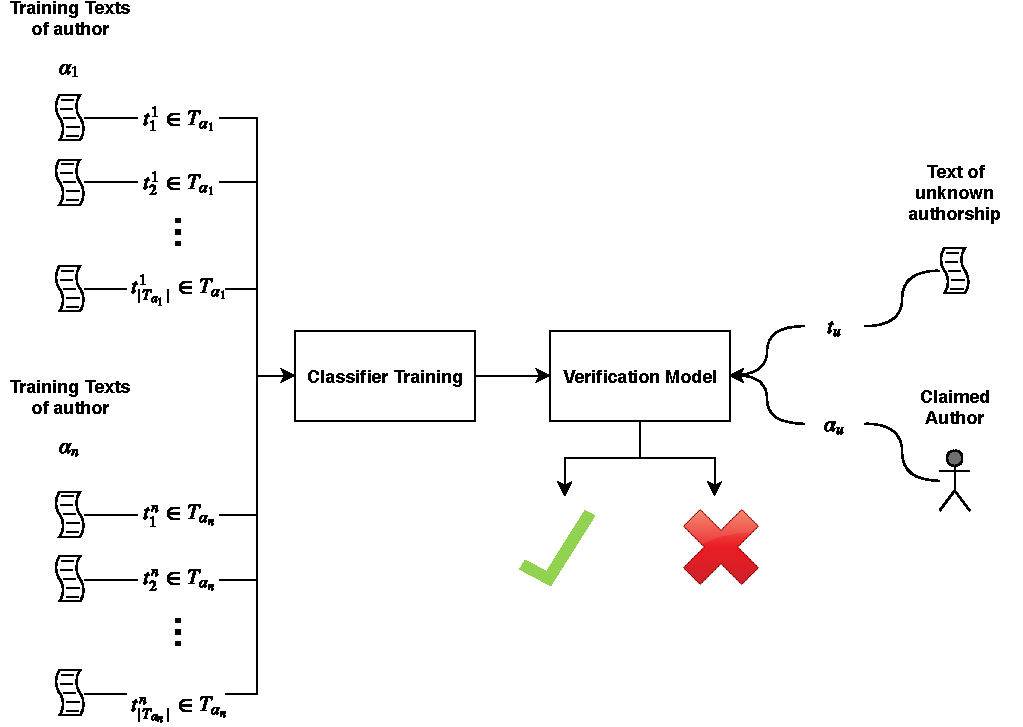
\includegraphics[width=\textwidth]{./pictures/method/instance_based}
    \caption{Illustrate the typical instance based authorship verification
    solution setup. Inspired by \citet{stamatos2009} a set of authors are given
    as input each with a set of texts. Some machine learning model is trained on
    the input texts and the model is used to predict an unknown text. $\alpha_u$
    denotes the proposed author the model checks $t_u$ against.}
    \label{fig:instance_based}
\end{figure}

\begin{figure}[htb]
    \centering
    \textbf{Profile Based Authorship Verification}\par\medskip
    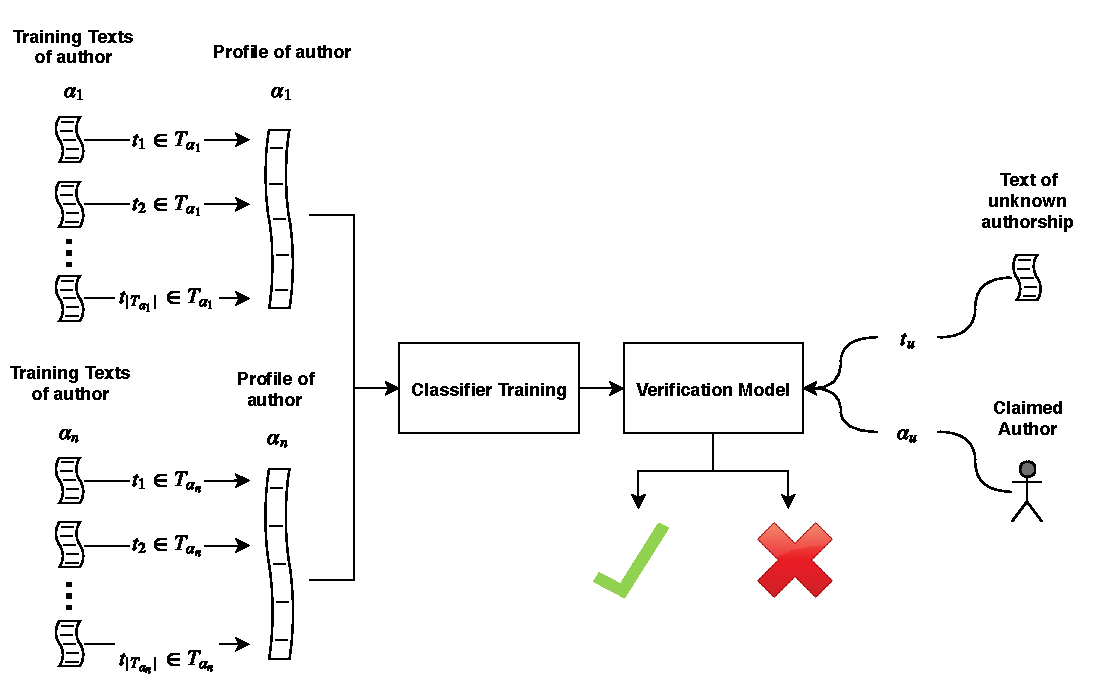
\includegraphics[width=\textwidth]{./pictures/method/profile_based}
    \caption{Illustrate the typical profile based authorship verification setup.
    Inspired by \citet{stamatos2009} the texts of each author are combined using
    some combination function such as an average or a concatenation. Those
    \textit{profiles} are then given to a Machine Learning model to train. The
    output is a model which is used to predict unknown texts. $\alpha_u$ denotes
    the proposed author the model checks $t_u$ against.}
    \label{fig:profile_based}
\end{figure}

\noindent An example of a profile-based authorship attribution approach, which
is highly regarded by \citet{stamatos2009} makes use of a compression algorithm.
It works not by representing each author profile as a set of features, but
rather as a set of compressed texts. In the initial scenario we have
a set of author-profiles for each author $\alpha$, where each profile is
the concatenation of all $t \in T_\alpha$. Authorship of a newly introduced
text is then determined by looping through each author adding the new text to
their concatenated profile. The profile is then compressed both with and without
the new text included. The bit-wise difference is then computed, by subtracting
them from one another resulting in what is essentially the cross-entropy between
the two sets. The author with the lowest cross-entropy is then considered to
be the author of this new text. Different methods of compression can be used
as the base for this model each giving different results. In the instance that
\citet{stamatos2009} describes, RAR compression yielded the best results, but
the choice of compression algorithm depends on the specific scenario.

We will generally use the instance based approach since it allows us to use more
metadata text information. For example the writing style of an author may change
over time especially for secondary school students that evolve a lot throughout
their school attendance. Since we use an instance based approach we are able
to weigh similarity to newer texts higher than similarity to older texts as
\citet{hansen2014} found worked well. The practical application of this will be
explained in Section \ref{subsec:combining_neural_network_output}.

There are also another split between methods that we consider. There are
generalizing and author specific models. In a generalizing model only a single
model is trained on data from multiple authors and are able to make predictions
about previously unseen authors. In the author specific model a separate model
has to be trained for each author and is not able to make predictions for
previously unseen authors. The generalizing models' main advantage is that it
only has to be trained once and after that it can be used for everyone. The
author specific model has the advantage that it can better fit to the specific
quirks of a particular author since it is trained separately for each author.
We will focus on the generalizing approach since it is more practical for
MaCom as they only have to train a model once.

In order to measure the quality of our models, we will also compute the
number of \glspl{TP}, \glspl{TN}, \glspl{FP} and \glspl{FN}, as seen in
\citet{US}. In these problems we get,

\begin{itemize}
    \item a \gls{TP} whenever we answer \textit{True} and the text is written
        by the claimed author,
    \item a \gls{TN} whenever we answer \textit{False} and the text is
        \textbf{not} written by the claimed author,
    \item a \gls{FP} whenever we answer \textit{True} and the text is
        \textbf{not} written by the claimed author,
    \item a \gls{FN} whenever we answer \textit{False} and the texts is written
        by the claimed author.
\end{itemize}

Given those definitions the \gls{TPR}, \gls{FPR}, \gls{TNR} and \gls{FNR}
are defined as follows.

\begin{description}
    \item[\gls{TPR}: ]

        The fraction of positives that we reported \textit{True} on i.e.~the
        fraction of texts written by the same author that we say are written by
        the same author.

    \item[\gls{TNR}: ]

        The fraction of negatives that we reported \textit{False} on i.e.~the
        fraction of texts written by different authors that we say are written
        by different authors.

    \item[\gls{FPR}: ]

        The fraction of negatives that we reported \textit{True} on i.e.~the
        fraction of texts written by different authors that we say are written
        by the same author.

    \item[\gls{FNR}: ]

        The fraction of positives that we reported \textit{False} on i.e.~the
        fraction of texts written by the same author that we say are written by
        different authors.

\end{description}

And they can be computed as,

\begin{align}
    TPR &= \frac{TP}{TP + FN}, \\
    FPR &= \frac{FP}{FP + TN}, \\
    TNR &= \frac{TN}{TN + FP}, \\
    FNR &= \frac{FN}{FN + TP}.
\end{align}

Using these definitions we can also describe the accuracy measure we will be
reporting on throughout our experiments,

\begin{equation}
    \text{Accuracy} = \frac{TP + TN}{TP + FP + TN + FN}.
\end{equation}

In the case of MaCom, we want to minimize the \gls{FNR} as much as possible,
so as to not wrongfully accuse anyone of handing in a ghostwritten assignment.
This however leaves out an equally important metric. While a low \gls{FNR} is
the goal, MaCom also wants to minimize the number of \glspl{FN} compared to the
total number of accusations made. This can be described as:

\begin{equation}
    \text{Accusation Error} = \frac{FN}{FN + TN}.
\end{equation}

The goal is also to keep this error under a certain threshold specified
by MaCom, which in this case is $0.1$ or $10\%$. In other words, of the
accusations we make, only $10\%$ of them are allowed to be wrong. In order
to accommodate this constraint we can take certain actions which depends on
the model used. Details about these actions will be addressed in Section
\ref{subsec:combining_neural_network_output}.

In addition to the constraint on the accusation error Macom also wants a
specificity above 95\%. Specificity is defined as,

\begin{equation}
    \text{Specificity} = \frac{TN}{TN + FP}.
\end{equation}

Specificity therefore represents the fraction of the total negatives we catch.
To catch 95\% of ghostwriters is a very ambitious goal. As described earlier it
is more important to keep the accusation error low than to catch many ghost
writers. We will therefore primarily focus on keeping the accusation error lower
than 10\% and then see how high we can get the specificity at the same time.

\subsection{Baseline Methods}

We have implemented two baselines to compare with our neural network methods.
The methods were selected based on our previous report \citep{US}. The methods
were developed for English texts and not Danish texts that we work with in
this assignment. They do however represent classical machine learning methods
for solving the authorship verification problem. They will therefore serve
as a great baseline for our neural networks. We believe that by changing the
parameters of the models they will work just as well for Danish texts that they
did on English texts. The Danish and English language is very similar as they
both derive from the Germanic branch of the Indo-European language family.
\citet{konstantin:2000} conducted a study of the similarities and differences
between different European languages. Based on a lexical distance computation,
he determined among other things that English and Danish are very similar. None
of the baseline methods work on raw texts. Rather they require hand engineered
feature sets extracted from the texts. The features used by \citet{US} were
all n-gram frequencies as in many classic authorship verification methods
\citep{stamatos2009}. We use the same features as described in our preliminary
report. We change the specific n-grams to n-grams extracted from Danish texts
but the classes of n-grams will stay the same. The n-grams come from several
linguistic layers. Specifically we use frequencies of character-n-grams,
special-character-n-grams, word-n-grams and \gls{POS}-tag-n-grams.

\begin{description}

    \item[Character-n-gram]

        Refer to character sequences of size $n$.

    \item[Special-character-n-grams]

        Refer to sequences of characters of size $n$ where all alphanumeric and
        space characters has been removed from a text. Special-character-n-grams
        can for example be used to find authors that use long sentences and
        therefore many commas in a row.

    \item[Word-n-grams]

        Refer to sequences of words of size $n$.

    \item[\gls{POS}-tag-n-grams]

        Refer to \gls{POS}-tag sequences of size $n$. A \gls{POS}-tag is the
        grammatical class of individual words such as nouns of adjectives. To
        extract \gls{POS}-tags from texts we use the \gls{POS}-tagger provided
        by \citep{polyglot}.

\end{description}

We will now describe shortly the two baseline methods we implemented.

\subsubsection{Extended Delta Method}

One of the best performing methods of \citet{US} was the extended delta method.
As the name suggests the method extends the already existing delta method
\citep{evert2015towards}. The original delta method verifies authorship of a
text by using a \gls{KNN} classifier. This \gls{KNN} is applied to the linearly
transformed word frequencies of the applied texts. The words, of which the
frequencies are found, are selected based on their frequency as well. So the
\gls{KNN} is trained using the frequency of a number of the most frequent words.
The amount of most frequent words to include can differ, the amount chosen by
\citep{evert2015towards} was 150. The linear transformation he applied was a
simple 0 mean and unit variance transformation.

The extension we applied to this methods, is simply option to use features
that aren't the word frequency. As mentioned we made use of this approach in
our earlier work \cite{US}. However, due to data-specific circumstances we
were not able to modify the K in \gls{KNN}. In these circumstances, that is not
the case. This leaves the extended delta method with 3 configurable parameters.
The features used, how many neighbor to consider denoted by K, and what distance
measure to use denoted by $p$. Where $p$ is the argument used when calculating
the Minkowski distance. The more known values for p is, $p = 1$ which is the
manhattan distance, and $p=2$ which is the Euclidean distance.

\subsubsection{Author Specific SVM}
\glsreset{SVM} 

Our other baseline method is the author specific \gls{SVM}. The method
was used in \citep{US} and was originally inspired by \citet{hansen2014}.
They used an \gls{SVM} on the Macom dataset as we described in Section
\ref{subsec:previous_work_using_macoms_dataset}. To verify the authorship of a
text $t$ and author $\alpha$ using this method, a two class \gls{SVM} classifier
has to be trained. The positive class is represented by features of each $t' \in
T_\alpha$ and the negative class is represented by the features of $t'' \in T$
where $T \subset \overline{T_\alpha}$ and $|T| = |T_\alpha|$. After training,
the classifier is used to predict if $t \in T_\alpha$ or $t \in T$.
Since a separate \gls{SVM} model is trained for each author it can learn
the specific authors' writing style from $T_\alpha$. In contrast it also learns
how the author does not write using $T$.

The method is based on an \gls{SVM} so we have to experiment
with the hyperparameters $C$ and $\gamma$.\cite[E-Chapter
8]{Abu-Mostafa:2012:LD:2207825}. We will find the best parameters via cross
validation. The parameter search will be described in detail in Section
\ref{sec:experiments}.


\subsection{Deep Learning}

In this paper we will approach the authorship verification problem using deep
learning. The term deep learning was first introduced to machine learning in
1989. The term deep learning quickly became synonymous with neural networks
as they were some of the more efficient and popular deep learning methods
\citep{Schmidhuber:2015}.

With the inner workings of the brain used as the basis, a standard simple
neural network consists of a set interconnected processors, called neurons.
Each of these neurons has a real valued activation associated with it, which
activates differently depending on the specific neuron. The input neurons
activate through perceiving the environment, or in other words, when they are
fed data externally. Other neurons are simply activated through the weighted
output of previous neurons \citep{DBLP:journals/corr/Schmidhuber14}.

Neural networks have been around since the 1940s. However, back then they were
merely variations of the linear regressors used at the time, and were not
very reminiscent of the networks one can see today. It was not until the late
1960s, early 1970s, that networks comparable to the more modern approaches
surfaced. Examples of such early works are \citep{ivakhnenko1973cybernetic}
and \citep{4308320}, which describe multi-layered feed forward supervised
neural network architectures. While the work described in \citep{4308320}
was indeed one of the first cases of the modern neural network, getting
the network to learn was still a problem, as the tweaking of individual
weights attributed to each neuron in the network was not trivial. Little
did they know that research to solve that problem was already in progress.
The basics of continuous \gls{BP} was initially described by
\citet{Kelley1960}, quickly followed by a simpler approach which used only
the chain rule by \citet{DREYFUS196230}. It was not until 1970 that
the modern version of \gls{BP} was described, using automatic differentiation
as its basis. This prompted an increase in \gls{BP} related research in
the following decades. As computational power increased in the 1990s and
2000s, so did the practical usage of \gls{BP}, and neural network in general
\citep{Schmidhuber:2015}. The application of \gls{BP} will be
described in Section \ref{subsubsec:training_a_network}.

\glsreset{CNN} 

Like with the history of authorship attribution research in this area of science
picked up more interest as we entered the modern computational age, and with
the introduction of the \gls{CNN}. \glspl{CNN} are based on the early work
described in \citet{TJP:TJP19681951215}. They showed that cats' and monkeys'
visual cortexes contain a set of neurons, each individually responding to a
receptive field, or area, of their field of view. Neighboring receptive fields
all have a certain amount of overlap but in the end a cohesive view is created.
This is what paved the way for neocognition in 1980 \citep{Fukushima1980},
the basis of \glspl{CNN} which looks at overlapping subsections of data.
\citep{Schmidhuber:2015}.


\subsubsection{Neurons}\label{sec:neurons}

As mentioned previously a neural network consists of a collection of neurons.
Each neuron is a simplified mathematical model which behaves much like neurons
in the brain. They receive, process and transmit information. Each neuron has a
set of inputs called $x_{j}$ one of which $x_{0}$ is a special bias input set
to 1 and a single output called $z_i$, where $i$ refers to the neuron and $j$
refers to the specific input to that neuron. Each neuron computes a weighted sum
of its inputs and applies an activation function $h$ to the weighted sum. The
weights are called $w_{ij}$ and the weight of the bias $w_{i0}$. The function
each neuron computes is,

\begin{equation}\label{eq:neuron}
    z_i = h(a_i) = h\left(
        \sum_{j = 1}^d w_{ij}x_j + w_{i0}
 \right) = h\left(
        \sum_{j = 0}^d w_{ij}x_j \right)
\end{equation}

where $d$ is the number of inputs to the neuron. A more intuitive model of such
a neuron can be seen in Figure \ref{fig:neuron}.

\begin{figure}[!tbp]
  \centering
  \begin{minipage}[b]{0.45\textwidth}
    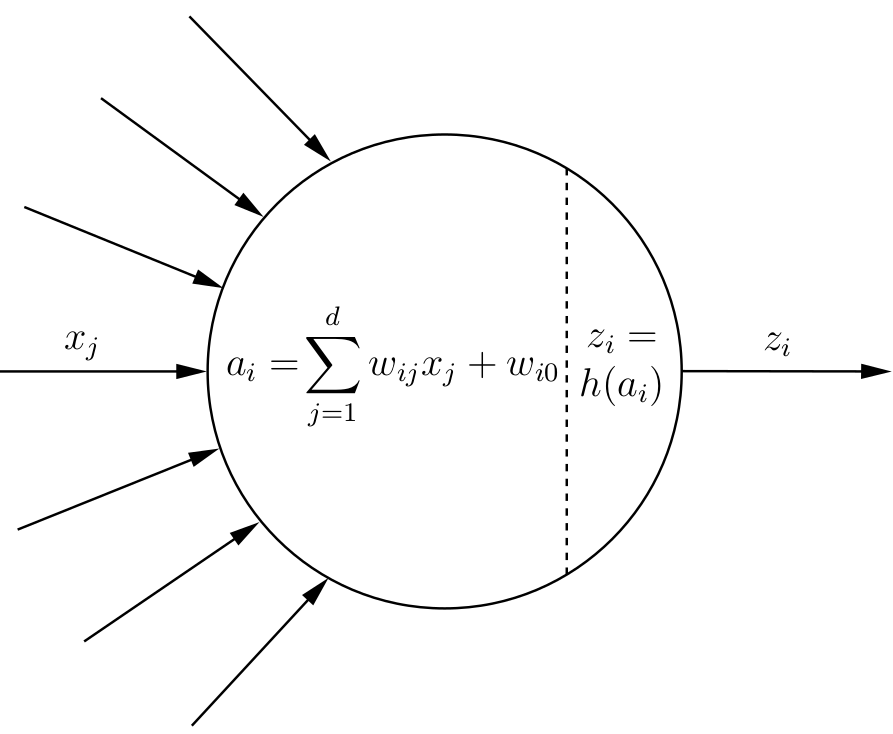
\includegraphics[width=\textwidth]{./pictures/method/neuron.png}
  \end{minipage}
  \hfill
  \begin{minipage}[b]{0.45\textwidth}
    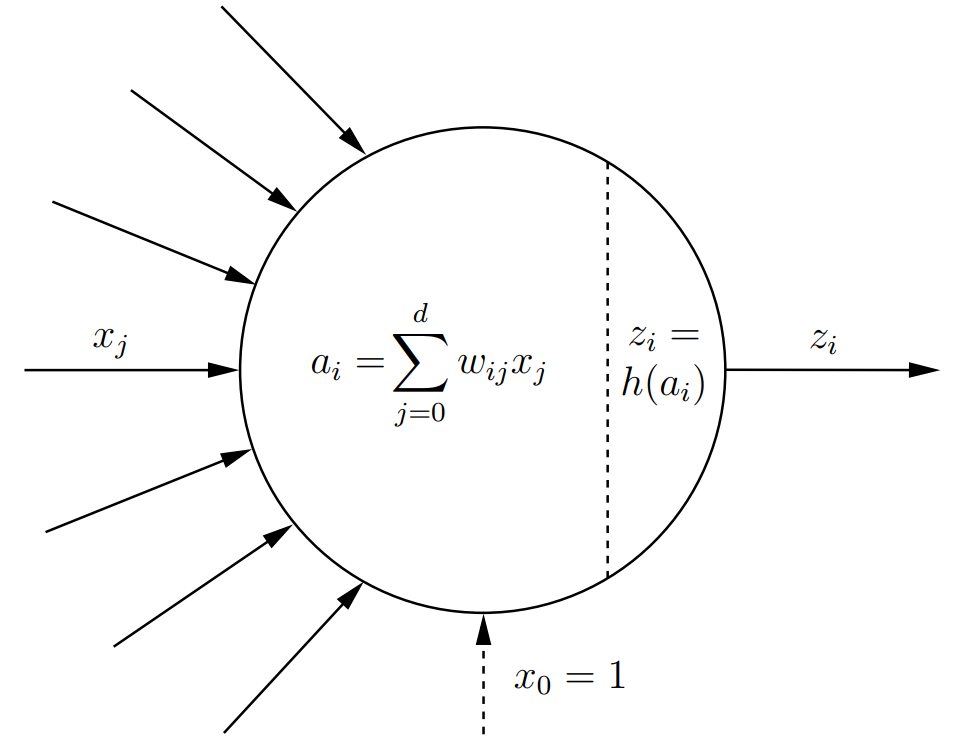
\includegraphics[width=\textwidth]{./pictures/method/neuron_bias.png}
  \end{minipage}
    \caption{The inner workings of a neuron, with and without an implicit
        bias \citep{Igel}. The left figure is without implicit bias while the
        right figure is with implicit bias.}
\label{fig:neuron}
\end{figure}

Neurons are usually arranged in layers in order to achieve a certain desired
behaviour. More details regarding these layers will be explained in
later chapters. The training of a neural network consists of changing the
weights applied at each neuron, with the goal of modeling the relationships
present in the data.


\subsubsection{Activation Functions} \label{subsubsec:activation_functions}

The activation function $h$, used at each neuron, defines the output of the
neuron given a certain input. A simple example of this would be computer chip
circuit, which can be seen as a series of activation functions outputting 0 or 1
depending on their input. This activation function would be a linear one. When
applying activation functions to neurons in neural networks, they are usually
non-linear, as it allows for the computation of more complex problems using a
smaller amount of neurons, relative to usage of a linear activation function,
as they allow for the universal function approximation, a point also made by
\citet{6797088} A plot of different activation functions is shown in Figure
\ref{fig:activation_functions}.

\begin{figure}
    \centering
    \textbf{Activation Functions}\par\medskip
    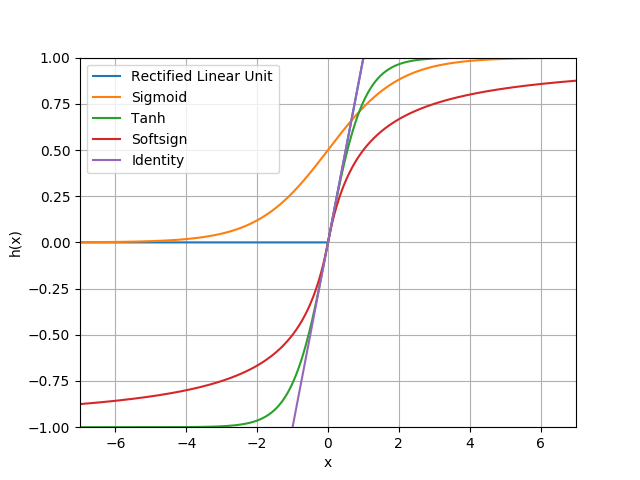
\includegraphics[width=0.5\textwidth]{./pictures/method/activation_functions.png}
    \caption{Different activation functions that can be used in neural
        networks.}
    \label{fig:activation_functions}
\end{figure}

Each activation function has its pros and cons. We mainly made use of the
\gls{ReLu} activation function in the layers of our networks. The reason for
this selection is its general purpose use. When selecting an activation function
for your neurons, the best function would be the one which best approximates
the underlying data relationship. Without a good idea as to what that function
might be, \gls{ReLu} is a good starting point. Its simplicity provides a quick
computation time, and its below zero limitation means that a large portion of
the network will not be activating, resulting in an even smaller computation
time. In addition to that, the derivative of the function is 1 in the case
of a positive input, resulting in the \gls{BP} loss having equal influence
throughout the network. In the case of other activation functions, this might
not be the case, resulting in an altering of the error as we propagate backwards
through the network. This could lead to a big error in the deeper layers not
reaching the shallow layers of the network. This property of the \gls{ReLu}
activation function, does however not come without its costs. If the learning
rate of the network is not configured correctly, a \gls{ReLu} activated neuron
might be blasted with a gradient so large, that it never reaches a point
of activation again. In other words, the neuron "dies". As such, one can
risk a network containing a lot of dead non-activating neurons, thus greatly
decreasing its learning quality. On the other hand the sigmoid activation
function does not allow its neurons to die. It can become victim to saturation.
In the case of a weight being too small or too large, the output values will
be placed at the far ends of the sigmoid range of values. At this point the
gradient is incredibly small, meaning that the contribution that neuron now
has is negligible. This neuron is now only a strain on the network, slowing
it down through its activation but contributing nothing - a problem \gls{ReLu}
does not have. Its based on these considerations we chose the \gls{ReLu}
activation function, leaving us the task of properly selecting our learning rate
\citep{JiYan, AndrejKarpathy, AvinashSharmaV}.

As the activation function of our output neurons we have used the softmax
function. The function is defined as

\begin{equation}
    h(x_i) = \frac{e^{x_i}}{\sum_{k=1}^n e^{x_k}}, \text{for $i = 1,\dots,n$}.
\end{equation}

The softmax function takes any vector $x \in \mathbb{R}^n$ and returns a vector
$y \in [0, 1]^n$. Where the sum of the output vectors elements will be equal to
1. The function is therefore great at constructing a probability distribution
based on an input vector.

Exceptions to usage of the \gls{ReLu} activation function can be found when
we make use \gls{LSTM} layers during our experimentation. It uses the
tanh activation function,

\begin{equation}\label{eq:tanh}
h(x) = \tanh(x) = \frac{(e^x - e^{-x})}{(e^x + e^{-x})}
\end{equation}

and the hard sigmoid activation function

\begin{equation}\label{eq:h_sig}
h(x) = \max(0, \min(1, x \cdot 0.2 + 0.5))
\end{equation}

These both serve as the default activations functions when using the keras deep
learning library. \cite{chollet2015keras}

\subsubsection{Layers} \label{subsubsec:layers}

Neural networks are organized in layers of neurons. The first layer is called
the input layer and is connected directly to the input of the model and the last
layer is called the output layer. The output of this layer is considered the
output of the entire network. All layers in between are called hidden layers.
A practical example could be where the input layer where each neuron took the
pixel of an image as the input. The output layer could then consist of a single
neuron that computes the probability that the picture contained a cat. An
example of a layered neural network are shown in Figure \ref{fig:example_nn}.

\begin{figure}
    \centering
    \textbf{Example Neural Network}\par\medskip
    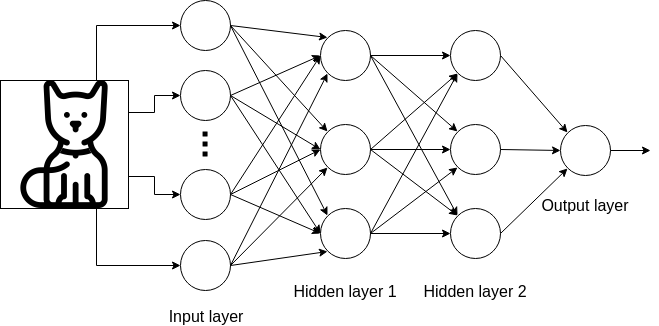
\includegraphics[width=\textwidth]{./pictures/method/example_neural_network}
    \caption{Example neural network that illustrates how neurons are organized
        into different layers with a special input layer, a special output layer
        and two hidden layers. The neurons in the input layer are connected to
        individual pixels in an input image and the output layer is a single
        neuron computing the probability that the image contains a cat.}
    \label{fig:example_nn}
\end{figure}

There are different kinds of layers. Below is a
non-exhaustive description of different layers, based on
\citep{oshea2015,DBLP:series/sci/2012-385,Goodfellow-et-al-2016,
mikolov2013linguistic,JMLR:v15:srivastava14a}.

\begin{description}

    \item[Dense Layer:]

        In a dense layer the input of each neuron in the layer is connected to
        the output of every neuron in the previous layer. Each neuron in the
        layer computes a weighted sum of the outputs of the previous layers'
        neurons and applies an activation function. The weights for each of
        the neurons in the layer are different allowing each neuron to learn a
        different combination of the previous layer. An example of this can be
        seen in Figure \ref{fig:example_nn}, where the hidden layers are Dense.

    \item[Convolutional Layer:]

        A convolutional layer is mainly used to extract position independent
        features from data. The convolution consist of a sliding window that
        slides over some input data and gives an output for each possible
        position in the input image. The sliding window uses the same weights
        in all the input and will therefore extract the same features from
        different locations if it is presented with the same input. The
        convolution computes a single output for each window position. The
        output is computed as the sum of the elementwise multiplication of
        the sliding window and the current part of the input it is looking at
        \citep{oshea2015}. Let us for example consider a two dimensional input,

        \begin{equation}
            X = \begin{pmatrix}
                1 & 1 & 1 & 0 \\
                1 & 0 & 0 & 1 \\
                0 & 1 & 0 & 1 \\
                0 & 0 & 1 & 0
            \end{pmatrix},
        \end{equation}

        and the convolutional filter,

        \begin{equation}
            w = \begin{pmatrix}
                1 & 0 & 0 \\
                1 & 0 & 0 \\
                0 & 1 & 0 \\
            \end{pmatrix}.
        \end{equation}

        Then we start the sliding window in the top left corner and compute the
        elementwise product of the matrices,

        \begin{equation}
            Y = X_{[1,3;1,3]} \otimes w =
            \begin{pmatrix}
                1 & 1 & 1 \\
                1 & 0 & 0 \\
                0 & 1 & 0
            \end{pmatrix} \otimes
            \begin{pmatrix}
                1 & 0 & 0 \\
                1 & 0 & 0 \\
                0 & 1 & 0
            \end{pmatrix} =
            \begin{pmatrix}
                1 & 0 & 0 \\
                1 & 0 & 0 \\
                0 & 1 & 0
            \end{pmatrix},
        \end{equation}

        to then compute the final value we take the sum of all the elements in
        that matrix,

        \begin{equation}
            \sum_{i,j} Y_{i,j} = 1 + 0 + 0 + 1 + 0 + 0 + 0 + 1 + 0 = 3.
        \end{equation}

        We then slide the window one to the right and repeat the same process,

        \begin{equation}
            Y = X_{[2,4;1,3]} \otimes w =
            \begin{pmatrix}
                1 & 1 & 0 \\
                0 & 0 & 1 \\
                1 & 0 & 1
            \end{pmatrix} \otimes
            \begin{pmatrix}
                1 & 0 & 0 \\
                1 & 0 & 0 \\
                0 & 1 & 0
            \end{pmatrix} =
            \begin{pmatrix}
                1 & 0 & 0 \\
                0 & 0 & 0 \\
                0 & 0 & 0
            \end{pmatrix},
        \end{equation}

        and the final value,

        \begin{equation}
            \sum_{i,j} Y_{i,j} = 1.
        \end{equation}

        We keep sliding the window right until we run out of input. After that
        we go back to the left and go one row down. We continue the process for
        all the input and we end up with the matrix,

        \begin{equation}
            O = \begin{pmatrix}
                \sum_{i,j} \left( X_{[1,3;1,3]} \otimes w \right)_{i,j} &
                \sum_{i,j} \left( X_{[2,4;1,3]} \otimes w \right)_{i,j} \\
                \sum_{i,j} \left( X_{[1,3;2,3]} \otimes w \right)_{i,j} &
                \sum_{i,j} \left( X_{[2,4;2,3]} \otimes w \right)_{i,j}
            \end{pmatrix} = \begin{pmatrix}
                3 & 1 \\
                1 & 2
            \end{pmatrix}.
        \end{equation}

        A visualization of this process can be seen in Figure
        \ref{fig:convolution_visualization}.

        \begin{figure}
        \centering
        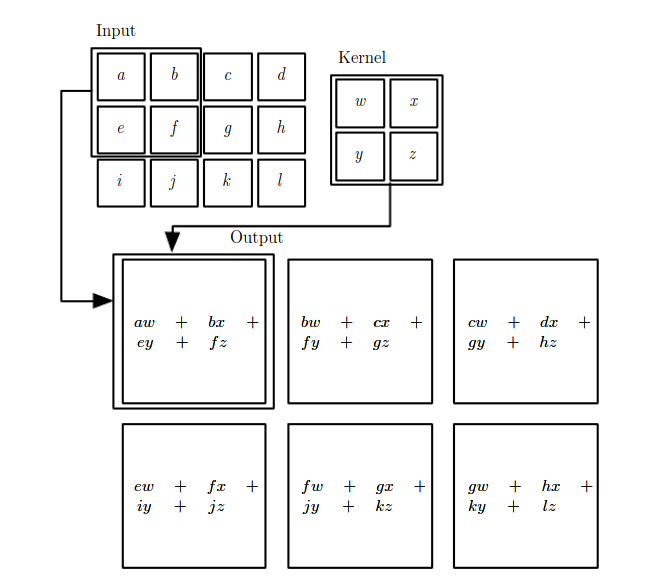
\includegraphics[width=0.6\textwidth]{./pictures/method/convolution_visualization.png}
        \caption{An example of 2D convolution, using a 2x2 kernel/sliding window
            size and a step size of 1 \citep{Goodfellow-et-al-2016}.}
        \label{fig:convolution_visualization}
        \end{figure}

        It can be seen that the output size is smaller than the input size. To
        prevent that the input can be padded with some value. A normal choice is
        zero padding. For the above input that would result in,

        \begin{equation}
            \begin{pmatrix}
                1 & 1 & 1 & 0 \\
                1 & 0 & 0 & 1 \\
                0 & 1 & 0 & 1 \\
                0 & 0 & 1 & 0
            \end{pmatrix} \xrightarrow{\text{zero padding}}
            \begin{pmatrix}
                0 & 0 & 0 & 0 & 0 & 0 \\
                0 & 1 & 1 & 1 & 0 & 0 \\
                0 & 1 & 0 & 0 & 1 & 0 \\
                0 & 0 & 1 & 0 & 1 & 0 \\
                0 & 0 & 0 & 1 & 0 & 0 \\
                0 & 0 & 0 & 0 & 0 & 0
            \end{pmatrix}.
        \end{equation}

        This would also make sure that edge values has the same amount of
        influence as the rest of the values. The sliding length can be
        different than one and is usually referred to as stride. The weights
        the convolutional window uses are learnable by the network. Certain
        convolutional filters can be used for edge detection and blurring the
        input. Some examples of different convolutional kernels applied to a
        grayscale image are shown in Figure \ref{fig:convolution_example}.

        \begin{figure}
            \centering
            \textbf{Examples of different convolutional kernels}\par\medskip
            \begin{tabular}{ccc}
                \textbf{Original} & \textbf{Kernel} & \textbf{Result} \\
                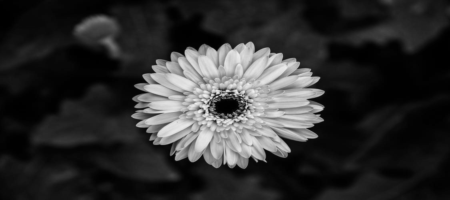
\includegraphics[width=0.3\textwidth]{./pictures/method/original_convolution.png} &
                \raisebox{1.2\height}{
                \begin{minipage}[b]{6cm}
                    \begin{equation*}
                        \begin{pmatrix}
                            1 & 0 & -1 \\
                            0 & 0 & 0  \\
                            -1 & 0 & 1
                        \end{pmatrix}
                    \end{equation*}
                \end{minipage}}
                    &
                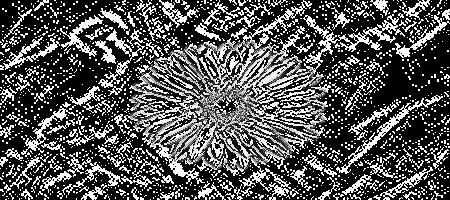
\includegraphics[width=0.3\textwidth]{./pictures/method/edge_detect_convolution.png} \\

                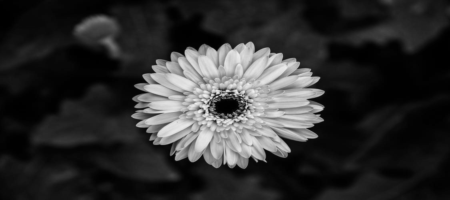
\includegraphics[width=0.3\textwidth]{./pictures/method/original_convolution.png} &
                \raisebox{1.2\height}{
                \begin{minipage}{6cm}
                    \begin{equation*}
                        \frac{1}{16}\begin{pmatrix}
                            1 & 2 & 1 \\
                            2 & 4 & 2  \\
                            1 & 2 & 1
                        \end{pmatrix}
                    \end{equation*}
                \end{minipage}}
                    &
                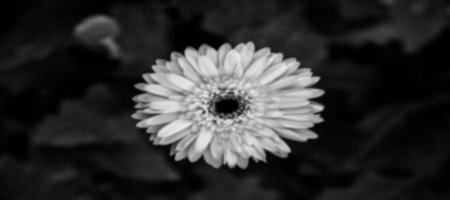
\includegraphics[width=0.3\textwidth]{./pictures/method/blurred_convolution.png} \\

                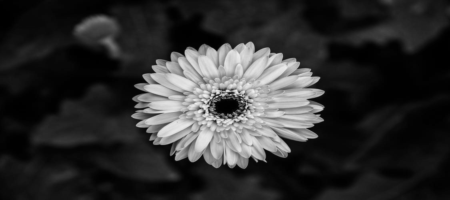
\includegraphics[width=0.3\textwidth]{./pictures/method/original_convolution.png} &
                \raisebox{1.2\height}{
                \begin{minipage}{6cm}
                    \begin{equation*}
                        \begin{pmatrix}
                            0  & -1 & 0  \\
                            -1 & 5  & -1 \\
                            0  & -1 & 0
                        \end{pmatrix}
                    \end{equation*}
                \end{minipage}}
                    &
                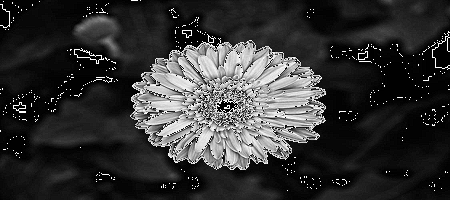
\includegraphics[width=0.3\textwidth]{./pictures/method/sharpened_convolution.png}
            \end{tabular}
            \caption{Examples of convolutional kernels applied to an image. The
                first kernel is an edge detect kernel, the second a blurring
                kernel and the third a sharpening kernel.}
            \label{fig:convolution_example}
        \end{figure}

        Convolutional layers for text analysis works slightly differently.
        Text is not two dimensional but one dimensional data. A convolution
        on text therefore does not use a two dimensional sliding window but
        a one dimensional one. The process is the same as before. The window
        slides over the text looking at a sequence of characters at a time. Each
        character is multiplied by the weight in that positition and a sum is
        computed. The output of the layer is a one dimensional sequence of these
        weighted sums. We will describe in more detail how convolutions for text
        work in Section \ref{subsubsec:conv_char_nn}.

    \item[\gls{RNN} Layer:]

        An \gls{RNN} network resembles a normal feed forward
        neural network except that it allows circular connections
        \citep{DBLP:series/sci/2012-385}. The circular connections can be used
        to remember previous inputs and an \gls{RNN} therefore has a sense of
        history of previous input and output. Classical feed forward neural
        networks can be viewed as mappings from and to vectors while \glspl{RNN}
        can be viewed as mappings from and to sequences. An \gls{RNN} does not
        view its input as a vector but as a sequence of inputs in different
        timesteps. We have shown an example of an \gls{RNN} network in Figure
        \ref{fig:rnn_illustration}.

        \begin{figure}
            \centering
            \textbf{Illustration of an \gls{RNN} Layer}\par\medskip
            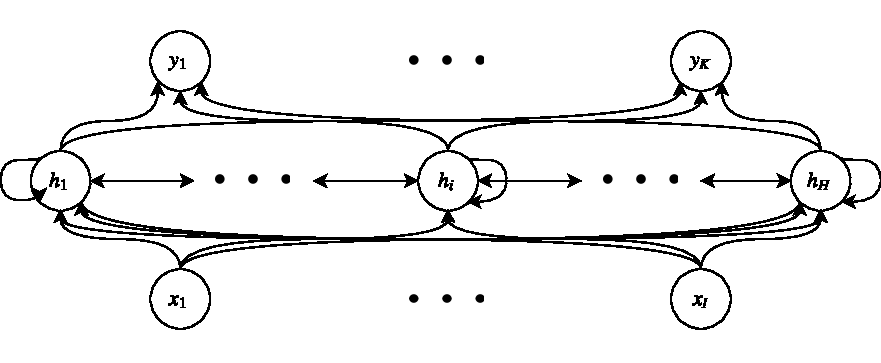
\includegraphics[width=\textwidth]{./pictures/method/RNN}
            \caption{Illustrates the structure of an \gls{RNN}. The \gls{RNN}
                consist of three layers, an input layer, a hidden layer and an
                output layer. The \gls{RNN} shown consist of $I$ input units,
                $H$ hidden units and $K$ output units. In the hidden layer each
                neuron is connected to every other neuron in the layer including
                itself.}
            \label{fig:rnn_illustration}
        \end{figure}

        In the forward pass of an \gls{RNN} network both the activations of
        the hidden units and the activations of the output units have to be
        computed. In the computation of the activation of the hidden units, the
        output of hidden units in the previous timestep are required. We let
        $a^{(t)}_h$ denote the activation of neuron $h$ in the hidden layer in
        timestep $t$. It is computed as,

        \begin{equation}
            a^{(t)}_h = \psi_h\left(
                \sum_{j=1}^I w_{hj} x^{(t)}_j +
                \sum_{h'=1}^H w_{hh'} a^{(t-1)}_{h'}
            \right),
        \end{equation}

        where $x_j^{(t)}$ is the j'th input at timestep t, $\psi_h$ is
        the activation function of the hidden unit, $I$ is the number of input
        units, $H$ is the number of hidden units and $w_{hj}$ is the weight
        between neuron $h$ and the $j$'th input to that neuron. The weight
        $w_{hj}$ and $w_{hh'}$ does not refer to the same weight even when $j =
        h'$. Instead we abuse notation such that $w_{hj}$ enumerates the weights
        between the input and hidden layer and $w_{hh'}$ enumerates the weights
        between the hidden layer neurons. That is the activation of a hidden
        unit is an activation function applied to a weighted sum of the current
        inputs and the activation of all hidden units in the previous timestep
        \citep{DBLP:series/sci/2012-385}. The output of the \gls{RNN} is then
        computed as,

        \begin{equation}
            y^{(t)}_k = \sum_{h=1}^H w_{hk} a_{h}^{(t)}.
        \end{equation}

        That is the output of an \gls{RNN} layer is a weighted sum of its
        hidden units. The complete sequence of hidden activations are computed
        by starting at time $t=1$ and calling the functions above until
        the end of the sequence is reached incrementing $t$ by one in each
        recursive call. The initial weight at of the hidden units can be any
        initialization value. The obvious choice is 0, however better results
        have been found using non zero initial hidden unit weight values
        \citep{DBLP:series/sci/2012-385}.

        A \gls{RNN} is normally trained using the \emph{backpropagation through
        time} algorithm. For data where the usage of time does not make sense
        and where the context from both sides of each timesteps is useful such
        as for text it is normal to use bidirectional \glspl{RNN}. Then both a
        forward and a backward pass are made through the sequence. The output
        of each network at each time step can then depend both on the context
        before and after the input.

    \glsreset{LSTM}
    \item[\gls{LSTM} Layer:]
        \label{layer:LSTM}

        As described the main benefit of \glspl{RNN} are their ability to use
        previous context to make predictions. Unfortunately the \gls{RNN}
        architecture described above in practise does not allow context from
        far away to influence current output. The problem is known as the
        vanishing/exploding gradient problem. When backpropagating through an
        \gls{RNN} network each timestep corresponds to a separate layer in a
        normal feed forward neural network. So for sequences of several thousand
        timesteps, backpropagation has to go through several thousand layers.
        The magnitude of the gradient will at each layer either increase up or
        decrease and through the hundreds or thousands of layers that leads to
        the gradient either blowing up exponentially or vanishing to nothing.
        In practise the main problem is the vanishing gradient and not the
        exploding gradient. The vanishing gradient means that weights early
        in the network are not updated according to the final output since
        the gradient has disappeared while backpropagating back to the early
        weights. Therefore the network will not learn to use context over long
        periods of time but only to use the local context around a particular
        timestep \citep{DBLP:series/sci/2012-385}.

        There are several solutions to that problem and one of them are
        \gls{LSTM} networks. \gls{LSTM} networks were introduced by
        \citet{Hochreiter:1997:LSM:1246443.1246450}. \gls{LSTM} networks are
        designed to be able to remember things over long periods of time, hence
        the name. They have several \gls{RNN} constructs with specific purposes.
        They have an \gls{RNN} responsible for computing the output given the
        current input and the previous activation as described before. They have
        an \gls{RNN} responsible for deciding what part of the input to ignore.
        They have an \gls{RNN} responsible for deciding what to forget from the
        current memory. Finally they have an \gls{RNN} responsible for deciding
        what part of the output to select as the current output of the unit
        \citep{DBLP:series/sci/2012-385}. We have showed the structure of an
        \gls{LSTM} in Figure \ref{fig:lstm}.

        \begin{figure}
            \centering
            \textbf{Structure of an \gls{LSTM}}\par\medskip
            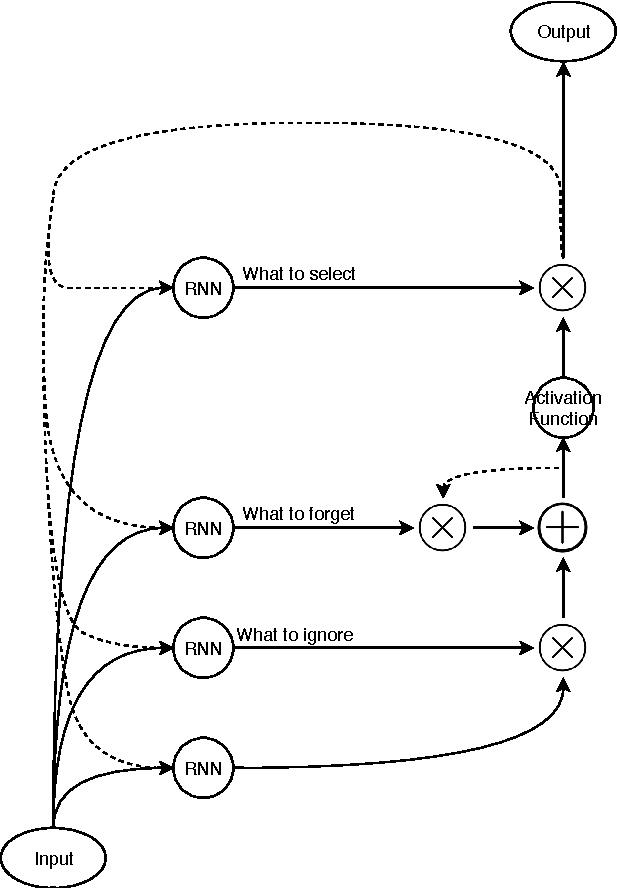
\includegraphics[scale=0.5]{./pictures/method/LSTM}
            \caption{The structure of an \gls{LSTM} network. $\bigoplus$ means
                an elementwise addition and $\bigotimes$ means an elementwise
                multiplication. Dotted lines show the movement of activations in
                the previous timestep while full lines show movement of the
                input in the current timestep.}
            \label{fig:lstm}
        \end{figure}

        The input to the \gls{LSTM} is fed into 4 \gls{RNN} networks that also
        receives the output from the previous timesteps. From bottom to top in
        the figure the \glspl{RNN} are:

        First: A network combining the current input and the previous output
        into an activation in the current timestep.

        Second: A network combining the current input and the previous output to
        compute which part of the activation of the first network to keep. The
        output of the second network is combined with the first network with an
        elementwise multiplication. That means that if the second network output
        a small value in a particular part of the output vector then that value
        will disappear from the output of the first network. The \gls{LSTM}
        therefore learns which part of the output to ignore.

        Third: A network combining the current input and the previous output
        to decide what to forget. The output of the network is combined with
        the current memory with an elementwise multiplication. So again if the
        network outputs a small value it can choose to forget a certain item.
        The network will learn when to throw things out of the current memory
        and when to keep them. The output of the elementwise multiplication is
        then combined with the current output via a elementwise addition. That
        allows the current memory to influence the output of the network. The
        added output and memory are transferred through an activation function
        that makes sure that nothing blows up and we get numerical instability.

        Fourth: A network combining the current input and the previous output
        to choose which values of the current output to select as the actual
        output. The output of the fourth network will be combined with the
        current model with an elementwise multiplication. So again the network
        can select which values to keep by outputting large numbers and which
        values to throw away by outputting small numbers. This network is the
        last applied to the output and can therefore select which values should
        be output.

    \item[Embedding:]

        The embedding layer maps a value into a continuous vector space. Given
        a sequence of integers, it uses the weights associated with the layer
        to map that each value to a vector of predetermined size. This can
        be done on any sort of data, as longs as it is encoded as a sequence
        of integers. In \gls{NLP} circumstances, this could be applied to
        characters or words for example, where each element in the sequence is
        first encoded as an integer value, and then fed to the embedding layer,
        which maps it to the continuous vector space. 
        Embedding layers are widely used in \gls{NLP}.

        The hope with using a layer such as this on characters, would be that
        each character got mapped to a point close to other similar characters,
        when the layer is properly trained. They are however mainly used
        to embed words. \citet{mikolov2013linguistic} found that embedding
        layers are able to learn more that just word similarities. They for
        example found that $vec("king") - vec("man") + vec("woman") \approx
        vec("queen")$ that is the embeddings learned the relation between the
        words king and queen and not just that they are similar words.

        \begin{figure}
            \centering
            \textbf{Example Character Embedding}\par\medskip
            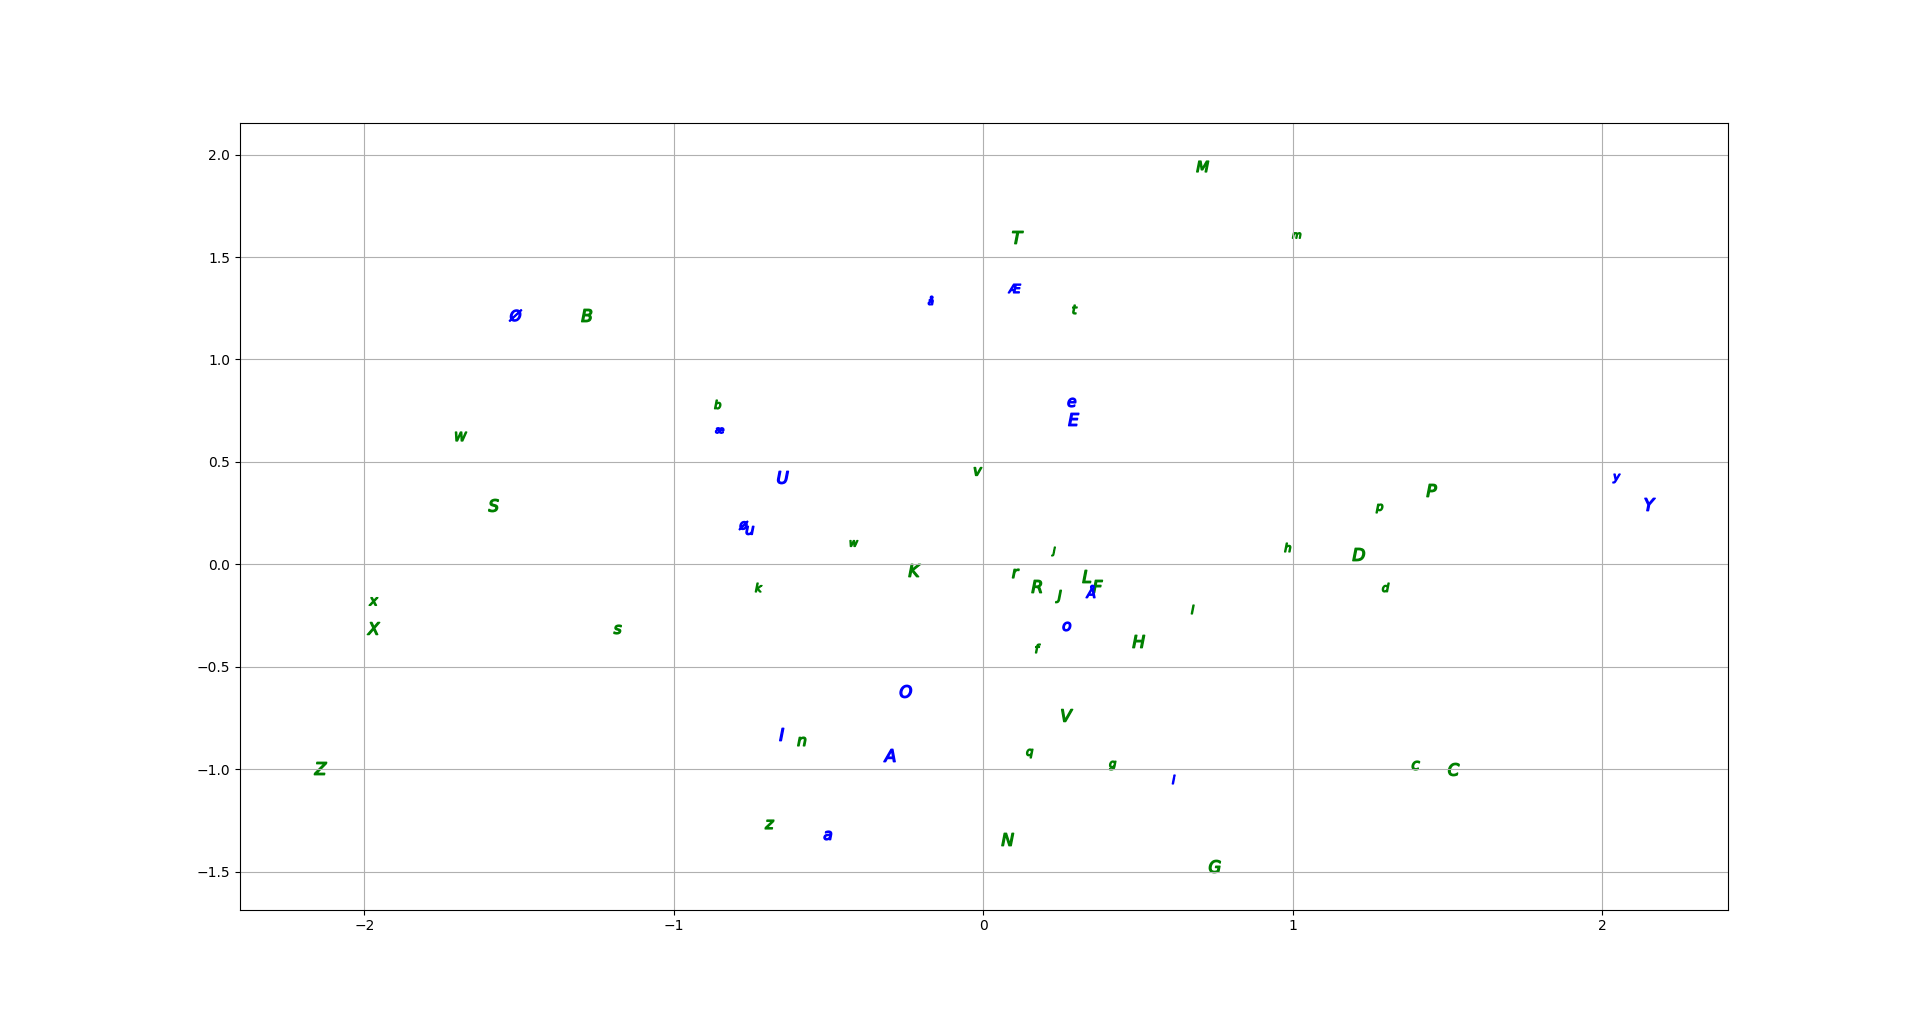
\includegraphics[width=\textwidth]{./pictures/method/example_character_embeddings.png}
            \caption{Character embeddings learned by a neural network. The
                embeddings were originally in 5 dimensional vectorspace and what
                is shown here is the first two principal components. Vowels are
                shown in blue and consonants in green.}
            \label{fig:embeddings}
        \end{figure}

        In Figure \ref{fig:embeddings} we have shown an embedding of one of our
        networks produces. The characters are embedded in 5 dimensions so the
        plot shows the first two principal components only. We can see that
        several lower and upper case letters have ended up close to each other.
        That means that the network has learned that those characters are
        interchangeable.

    \item[Pooling Layer:]

        The purpose of a pooling layer, or down-sampling layer, is as the name
        suggest, to pool the data it receives. It does so with the goal of
        distilling the data down to a number of key features found within said
        data. This of course decreases the computation time of the network as a
        whole, and with a smaller amount of parameters, comes a smaller chance
        of overfitting and a reduction in training time.

        Working in similar fashion as the convolutional layer, the max pooling
        layer also uses a sliding window. This sliding window of a certain
        dimensionality, is moved over the data given to it. The maximum value
        inside that window is then extracted, and set as the output for that
        specific window placement.  The window then moved a specified
        stride size, and the process is repeated. The result is a dataset which
        is down-sampled in proportion with the sliding windows dimensions, and
        the stride. An example of this max pooling process can be seen in Figure
        \ref{fig:max_pool}.

        Pooling layers are however not restricted to only the max pooling
        layer. The average pooling layers works in a very similar fashion,
        but instead of extracting the max value it simply averages values
        currently in the window. The Global Max Pooling Layer, which we use
        quite frequently in our networks does not use a window like the other
        ones described, but instead simply extracts the maximum value across
        the data the layer is provided, thus eliminating the need for a sliding
        window.

        \begin{figure}
        \centering
        \begin{equation}
            \begin{tabular}{|llll|}
            \hline
            1 & 8 & 7 & 2 \\
            9 & 7 & 9 & 8 \\
            3 & 6 & 2 & 4 \\
            5 & 7 & 9 & 9 \\\hline
            \end{tabular}
                \Longrightarrow
            \begin{tabular}{|ll|ll|}
            \hline
            \cc{blue}1 & \cc{blue}8 & \cc{red}7 & \cc{red}2 \\
            \cc{blue}9 & \cc{blue}7 & \cc{red}3 & \cc{red}8 \\ \hline
            \cc{orange}3 & \cc{orange}6 & \cc{green}2 & \cc{green}4 \\
            \cc{orange}5 & \cc{orange}7 & \cc{green}9 & \cc{green}9\\
            \hline
            \end{tabular}
                \Longrightarrow
            \begin{tabular}{|l|l|}
            \hline
            \cc{blue}9 & \cc{red}8\\\hline
            \cc{orange}7 & \cc{green}9\\
            \hline
            \end{tabular}
        \end{equation}
        \caption{An example of a max pooling performing using a 2x2 kernel and
            stride 2.}
        \label{fig:max_pool}
        \end{figure}


    \item[Dropout Layer:]

        This layer is used for regularization of neural networks. A well
        designed network combined with a good optimizer will, when given time,
        slowly become more and more fit on the training data it is provided.
        This is all dine, as long as what it learns is not specific to that,
        and only that, training data. If that is the case, then the network
        would be considered overfitted on the training data. In this case,
        the network does not properly generalize. This the problem that the
        dropout layer attempts to combat. It does so by deactivating a certain
        fraction of randomly selected neurons in a specified layer, for each
        training sample. This forces the model to learn from a larger set of
        sparse neurons, rather than a very small amount of neurons that only
        contribute dataset specific information. Since the network suddenly
        can not rely on the existence of these very informative data specific
        neurons, it has to learn based from less informative but more general
        neurons instead. The hope is that learning on more general data, results
        in a more generalizing model. An example of this can be seen in Figure
        \ref{fig:dropout}.

        \begin{figure}
            \centering
            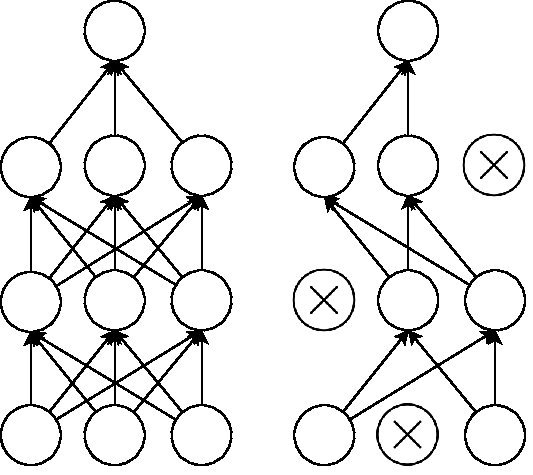
\includegraphics[width=0.5\textwidth]{./pictures/method/dropout}
            \caption{An example of the application of a dropouts being performed
                on different layers.}
            \label{fig:dropout}
        \end{figure}

        \citet{JMLR:v15:srivastava14a} investigated the use of dropout layers
        in different problem settings. They found that dropout layers reduced
        overfitting in all problems they looked at. In particular they found
        that document classification was also improved. The main drawback of a
        dropout layer is that it increase the training time of the networks its
        used on \citep{JMLR:v15:srivastava14a}.

\end{description}


\subsubsection{Training a Network} \label{subsubsec:training_a_network}

A neural network learns by updating the weights in the network. The weights are
updated using \textit{gradient descent} \citep{Bishop}. Gradient descent is
a method that can minimize any differentiable function by taking small steps
towards a local minimum. The function we minimize in a neural network is an
error function. The error function describes a quantity which when minimized
gives the network the best performance possible. Since gradient descent works
for any differentiable function the error function can be any function that is
differentiable. As an example consider the error function,

\begin{align}
    E(W)   &= \sum_{n=1}^{N} E_n(W) \\
    E_n(W) &= \frac{1}{2} \left( \hat{y}_n - y_n \right)^2
\end{align}

where $N$ is the number of training samples, $\hat{y}_n$ is the predicted
results, $y_n$ is the target, and $W$ is a set of weights. The gradient is
a multi-variable generalization of the derivative of a function. It is a
vector that points in the direction of steepest ascend in value for a function
at a specific point. Gradient descent is based on the observation that a
differentiable function $f$ in point $\mathbf{x}$ decrease fastest in the
direction of the negative gradient of the point $\mathbf{x}$ \citep{Bishop}.
That leads to a simple update rule that can be applied continuously to reach a
local minimum,

\begin{equation}
    \mathbf{x}_{n+1} = \mathbf{x}_n - \eta \Delta f\left(\mathbf{x}_n\right),
\end{equation}

where $\eta$ is a small number that makes sure we do not overstep the local
minimum. An example of the gradient descent process can be seen in Figure
\ref{fig:gradient_descent}. Our only real parameter we can change in order
to minimize an function are the weights $\mathbf{w}$. These can be changed
by using the gradient descent update rule,

\begin{figure}
    \centering
    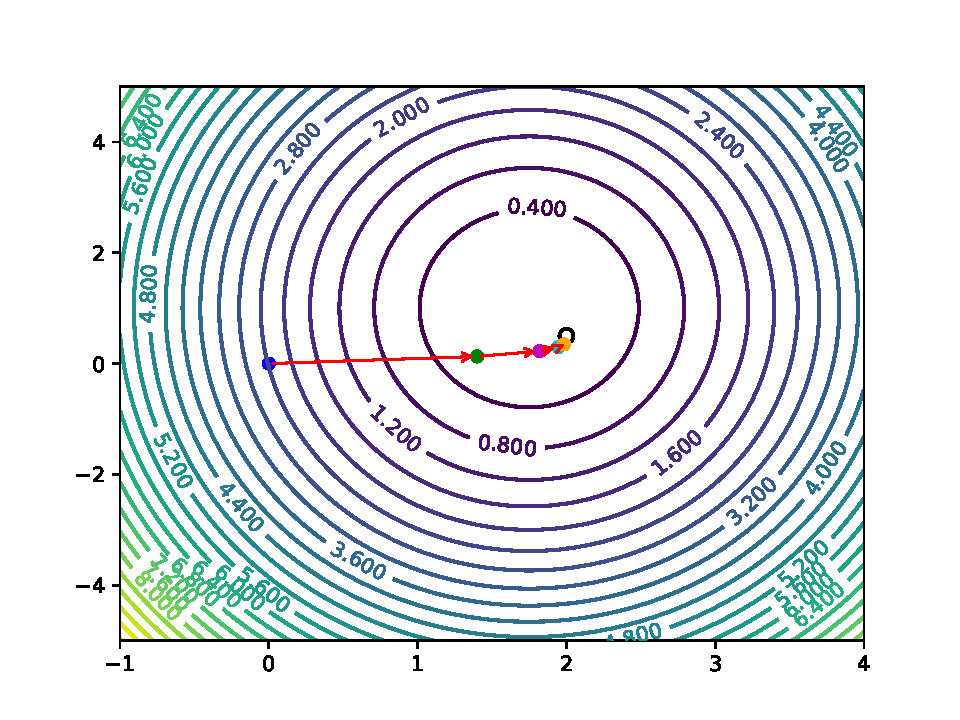
\includegraphics[width=0.8\textwidth]{./pictures/method/gradient_descend}
    \caption{An illustration of how gradient descent works. Each iteration steps
        in the direction of the local minimum of the specific function used,
        which in this case is signified by a black ring. The Figure is generated
        using code from
        \url{https://scipython.com/blog/visualizing-the-gradient-descent-method/}.}
    \label{fig:gradient_descent}
\end{figure}

\begin{equation} \label{eq:gradient_descent_network_update}
    \mathbf{w}^{(t+1)} = \mathbf{w}^{(t)} + \eta \Delta \mathbf{w}^{(t)},
\end{equation}

where $t$ is the timestep of the update and,

\begin{equation}
    \Delta \mathbf{w}^{(t)} = -\nabla E|_{\mathbf{w}^{(t)}}.
\end{equation}

$\nabla E|_{\mathbf{w}^{(t)}}$ refers to the gradient of the error function
relative to the specific weight vector $\mathbf{w}^{(t)}$, or rewritten,

\begin{equation}
    \nabla E|_{\mathbf{w}^{(t)}} = \frac{\partial E}{\partial \mathbf{w}^{(t)}}.
\end{equation}

Now we have an update rule for the weights of the network that will minimize an
error function $E$ chosen by us. We can choose $E$ as any function we and our
network desires as long as it is differentiable. The only problem left is how to
compute the gradient of the network. The computation of the gradient can be done
via the \gls{BP} algorithm \cite{Bishop}. \Gls{BP} depends on the activation
of all neurons to a specific sample. That gives us a three step algorithm for
updating the weights of the network.

\begin{description}
    \item[Feed Forward] Give input to first layer in network computing the
        activation of all neurons to that specific input.
    \item[Back Propagate] Use the \gls{BP} algorithm to compute the gradient of
        the network.
    \item[Update Weights] Use gradient descent to update the weights of the
        network.
\end{description}

The computation of the gradient starts at the error function $E$. For
simplicities sake we focus on only a single training sample and fix $E$ as,

\begin{equation}
    E = \frac{1}{2}(\hat{y} - y)^2.
\end{equation}

As mentioned we want to determine the gradient of this with respect to all the
weights in our network $w_{ij} \in W$. In order to do that we need to find
partial derivatives for those same weights and since each specific weight is
tied to a specific neuron we need to differentiate the entire network. But
before doing so, we need to establish the chain rule.

\begin{lemma}[Chain Rule]
\label{lemma:chainrule}

    If functions $f$ and $g$ are both differentiable and $F$ is the composite
    function defined by $F(x) = f(g(x))$, then $F' = f'(g(x)) \cdot g'(x)$,

\end{lemma}

The reason we need of the chain rule is that the loss function is essentially
a chain of function calls that spans the entire network. This fact becomes
apparent when we attempt to evaluate our single sample error function $E$ with
respect to a weight $w_{ij}$. If we keep in mind that the neurons in feed
forward neural networks computes a weighted sum of its inputs as per $a_i$ in
Equation \eqref{eq:neuron}. Then we known that $E$ only depends on $w_{ij}$
through the call of $a_i$, and it is for that reason what we can apply the chain
rule to get the following,

\begin{equation}
    \label{eq:bp_start}
    \frac{\partial E}{\partial \mathbf{w}_{ij}} = \frac{\partial E}{\partial a_i}
    \frac{\partial a_i}{\partial \mathbf{w}_{ij}}.
\end{equation}

We can add a little extra notation, which we will use hence forth, for the
sake of easing understanding,

\begin{equation}\label{eq:delta}
    \delta_i = \frac{\partial E}{\partial a_i}.
\end{equation}

$\delta$ is often referred to as the \textit{error} of a specific neuron.
From Equation \eqref{eq:neuron} we get that,

\begin{align}
    \frac{\partial a_i}{\partial \mathbf{w}_{ij}}
        &= \frac{\partial}{\partial \mathbf{w}_{ij}}
            \sum_{m=1}^d \mathbf{w}_{im} x_m + \mathbf{w}_{i0}\\
        &= \frac{\partial}{\partial \mathbf{w}_{ij}} \sum_{m = 0}^d
            \mathbf{w}_{im} x_m\\
        &= x_j.
\end{align}

Notice that we exchanged the $j$ counter in Equation \eqref{eq:neuron} with $m$
since we would otherwise have a name clash. That equation when combined with
Equation \eqref{eq:bp_start} gives us,

\begin{equation} \label{eq:deriv}
    \frac{\partial E}{\partial \mathbf{w}_{ij}} = \delta_i x_j.
\end{equation}

That reveals that the derivative of the cost function with respect to the weight
$\mathbf{w}_{ij}$ is simply the value of $\delta$ for the neuron at the output
end and $x$ for the input end of the weight for that same neuron. This leaves us
with calculating $\delta_i$ for the hidden units, and the output units of the
network. We already know that for output units $\delta$ is computed as,

\begin{equation}
    \label{eq:output}
    \delta_k = \hat{y}_k - y_k,
\end{equation}

where $k$ refers to a specific output neuron. For the hidden units the chain
rule has to be used again,

\begin{equation}
    \label{eq:bp}
    \delta_i = \frac{\partial E}{\partial a_i} =
    \sum_k \frac{\partial E}{\partial a_k} \frac{\partial a_k}{\partial a_i},
\end{equation}

Where the sum runs over all $k$ units $i$ outputs to. The Equation can be
rewritten using the prior established equalities and the chain rule,


\begin{align}
    \sum_k \frac{\partial E}{\partial a_k} \frac{\partial a_k}{\partial a_i}
    &= \sum_k \delta_k \frac{\partial a_k}{\partial a_i}
    & \text{By Equation \eqref{eq:delta}}
    \\
    &= \sum_k \delta_k \frac{\partial a_k}{\partial z_i}
        \frac{\partial z_i}{\partial a_i}
    & \text{By Equation \eqref{eq:neuron} and Lemma \ref{lemma:chainrule}}
    \\
    &= \sum_k \delta_k h'(a_i) \frac{\partial a_k}{\partial z_i}
    \\
    &= \sum_k \delta_k h'(a_i) \left( \frac{\partial}{\partial z_i}
        \sum_{j} \mathbf{w}_{kj} z_j\right)
    \\
    &= \sum_k \delta_k h'(a_i) \mathbf{w}_{ki}
    \\
\end{align}

This highlights that changes in $a_i$ only influences the error-function,
through variations of the variables $a_k$. We can compute the $\delta$ for a
particular hidden unit by backpropagating the $\delta$ value back from higher up
in the network.

As such, we can summarize the weight updating algorithm as,

\begin{enumerate}
    \item

        Provide the network with some input data $x_n$, and compute the
        activations of each hidden and output neuron using Equation
        \eqref{eq:neuron},

    \item

        Compute $\delta_n$ for each of the output neurons using Equation
        \eqref{eq:output},

    \item

        Back propagate $\delta$s using Equation \eqref{eq:bp} to compute
        $\delta_i$ for each neuron,

    \item

        Use Equation \eqref{eq:deriv} to evaluate the required derivatives.

    \item

        Update the weight using the computed derivatives
        and the gradient descent update rule from Equation
        \eqref{eq:gradient_descent_network_update}.

\end{enumerate}

These three steps feed forward, backpropagate and update weights are repeated
throughout the training cycle of the neural networks. Such that the weights are
optimized after each full parse over the training dataset.

The process described above is pretty computationally expensive, with a
time-complexity of $O(W)$. However, this is only the case when we are using
a singular training sample. If this process is to be done for each training
sample, the runtime would then be $O(N\cdot W)$, where $N$ denotes the total
number of training samples. During the normal training process, this is done
over a number of epochs $\mathcal{E}$, which in turn further increases the
time-complexity to $O(\mathcal{E}\cdot N\cdot W)$. It is because of this
runtime, that \gls{BP}, and neural networks might not seem like a viable option
at all \cite{Bishop}. 

There is however ways to improve the runtime. Both \textit{stochastic gradient
descent} and its' variation \textit{stochastic minibatch gradient descent},
attempt to alleviate this problem by reducing the size of $\mathcal{E}$. A more
detailed description can be found in the next Section. \citet{Bishop} does
present other alternatives in his book, but none work as well as these two
methods, which is why that is the default approach for neural network frameworks
such as Tensorflow/Keras.

%In light of this undesired runtime, methods were introduced that attempt
%to reduce this runtime. One of these methods is called batching. Batching
%first shuffles, and then splits the training data into smaller batches. Each
%individual batch is then run through the network, after which \gls{BP} is
%applied. Running \gls{BP} on this smaller batch means that the resulting
%gradient is only an approximation. Each epoch still consists of giving all $N$
%samples to the network, but now \gls{BP} is applied several times during an
%epoch, rather than after. This means that using batching greatly reduces the
%amount of $\mathcal{E}$ needed for the same amount of convergence provided
%by the non-batching approach, reducing overall run-time.\cite{Bishop} A
%more detailed description of this approach will be addressed in Section
%\ref{subsubsec:optimizers}.


\subsubsection{Optimizers}\label{subsubsec:optimizers}

Traditional gradient descent has been updated with several different algorithms.
These algorithms are called \textit{optimizers}. A good optimizer algorithm
will reach a local minimum faster than traditional gradient descent. The first
optimizer algorithm we will discuss is the \textit{stochastic gradient descent}
algorithm. In the traditional gradient descent we have described a single
weight update require computing the gradient of the error function on each
training sample. Often such a detailed gradient is not needed in practise.
Stochastic gradient descent is an attempt at estimating the gradient of all
datapoints using only a single datapoint. That means that in stochastic gradient
descent weights are updated much more often and is updated on a noisy target
\citep{Bishop}. The advantage of stochastic gradient descent is that convergence
to a local minimum might be much quicker since the algorithm does not have to
go through all training samples for each weight update. The weight updating for
stochastic gradient descent is computed as,

\begin{equation}
    \mathbf{w}^{(t+1)} =
        \mathbf{\mathbf{w}}^{(t)} -
        \eta\Delta E_n|_{\mathbf{w}^{(t)}}.
\end{equation}

In practise each weight update in stochastic gradient descent are computed
not based on a single training sample but on some small number of training
samples. That allows the computation to take advantage of highly optimized
matrix libraries and making each update on a slightly less noisy target
\footnote{\url{http://ufldl.stanford.edu/tutorial/supervised/OptimizationStochas
ticGradientDescent/}}. The version of stochastic gradient descent that use more
than one sample per weight update is known as stochastic minibatch gradient
descend.

To see how stochastic gradient descent might lead to faster convergence consider
a dataset with some number of training samples. To create redundancy in the
dataset we copy all training samples in the dataset to create a new dataset of
twice the size. In classical gradient descent the only effect will be that the
error increases by a magnitude of 2 but will take twice as long to compute.
While stochastic gradient descent will converge at the exact same speed as each
minibatch will still represent an estimate of the true underlying function and
each weight update still takes the same amount of time \citep{Bishop}.

Another advantage of the stochastic method is that the optimizer might escape
from a non optimal local minima and reach a better local minima. To see why that
might happen consider the fact that each minibatch consist of a different subset
of training samples. Even though when computed on all training samples the
gradient points towards the non-optimal local minima the gradient of a single
batch might point towards a better local minima. Therefore the optimizer has the
possibility of following the gradient of single batches that leads to a final
better local minima \citep{Bishop}.

A problem in the stochastic gradient descent algorithm is the need to choose
the learning rate $\eta$. If the learning rate is too high the algorithm
will diverge and if it is to low it will be very slow to converge. Therefore
several extensions to basic stochastic gradient descent has been developed that
automatically tunes the learning rate $\eta$. We will discuss three different
extension \gls{AdaGrad}, \gls{RMSProp} and \gls{Adam}.

In the description of those three algorithms we will slightly abuse vector
notation. Given $\mathbf{a}, \mathbf{b} \in \mathbb{R}^n$ we will keep using
$\mathbf{a} \otimes \mathbf{b}$ to mean an elementwise multiplication but
besides that we use $\frac{\mathbf{a}}{\mathbf{b}}$ to mean an elementwise
division, $\sqrt{\mathbf{a}}$ to mean an elementwise square root and
$\mathbf{a}^n$ to mean an elementwise power.

\begin{description}

    \item[\gls{AdaGrad}:]

        The algorithm was invented by \citet{Duchi:2011:ASM:1953048.2021068}.
        The algorithm attempts to solve the problem of choosing a learning
        rate and the problem of how to handle parameters that are infrequently
        activated. When a parameter is only infrequently activated the gradient
        on that parameter will often be close to 0. Infrequently used parameters
        are often the most important parameters for a classification task but
        since they are infrequent they are hard to learn on. \gls{AdaGrad}
        assigns a separate learning rate to each separate parameter. The
        algorithm gives infrequently observed parameters a very high learning
        rate and frequently observed parameters a very low learning rate. The
        method incorporates knowledge of the data from previous iterations to
        make choices in the current iteration. In \gls{AdaGrad} the weight
        update function is,

        \begin{equation}
            \mathbf{w}^{(t+1)} =
                \mathbf{w}^{(t)} -
                \eta \text{diag}\left(G^{(t)}\right)^{-\frac{1}{2}} \otimes
                \Delta E|_{\mathbf{w}^{(t)}},
        \end{equation}

        where $G^{(t)}$ is a matrix containing the sum of the outer product
        of the gradient in all previous timesteps $1, \dots, t$ and
        $\text{diag}(X)$ is the diagonal vector of the matrix $X$. $G^{(t)}$ is
        defined as,

        \begin{equation}
            G^{(t)} = \sum_{t'=1}^t \Delta E|_{\mathbf{w}^{(t')}}
                \left(
                    \Delta E|_{\mathbf{w}^{(t')}}
                \right)^T.
        \end{equation}

        For the updating of a single weight $w_i$ the above becomes
        \citep{Duchi:2011:ASM:1953048.2021068},

        \begin{equation}
            \label{eq:individual_adagrad}
            \mathbf{w}_i^{(t+1)} =
                \mathbf{w}_i^{(t)} - \frac{\eta}{\sqrt{G^{(t)}_{ii}}} \otimes
                \Delta E|_{\mathbf{w}_i^{(t)}}.
        \end{equation}

        $G_{ii}$ works as a scaling factor for weight $\mathbf{w}_i$.
        Since $\sqrt{G_{ii}} = \sqrt{\sum_{t'=1}^t \left(\Delta
        E|_{\mathbf{w}^{(t')}_i}\right)^2}$, $G_{ii}$ is the L2 norm
        of the gradient in the previous timesteps. That means that if the
        gradient has generally been large for a particular weight the norm
        will be large and the updating of the weight will be scaled down
        (slower) which can be seen in Equation \eqref{eq:individual_adagrad}.
        Similarly when the gradients of a weight has been small or 0 the
        weight is scaled less down and the upgrade will be larger. That has
        the effect of having infrequent parameters of the model train faster
        \citep{Duchi:2011:ASM:1953048.2021068}.

    \item[\gls{RMSProp}:]

        \gls{RMSProp} was introduced by Geoff Hinton in lecture 6e of his
        Coursera Class \citep{DBLP:journals/corr/Ruder16}. This section is based
        primarily on his slides \citep{HintonSrivastavaSwersky2014}. The idea
        behind \gls{RMSProp} is similar to \gls{AdaGrad} each weight is updated
        at an independent rate. Unlike \gls{AdaGrad} the rate is chosen by a
        moving average instead of the L2 norm of all previous steps. That allows
        the algorithm to adapt quickly to changes in the gradient. When the
        gradient of a weight is large the algorithm decreases the learning rate
        and when the gradient is consistently small it tunes up the learning
        rate. That functions well since a large gradient is found in a steep
        volatile area while a consistently small gradient is found in a flat non
        volatile area. In the steep areas we are likely to overshoot the target
        if the learning rate is to high while in flat areas we do not have that
        problem. The internal state of the algorithm is a vector $\mathbf{v}$
        of the running average of gradient magnitudes. It is updated with the
        equation,

        \begin{equation}
            \label{eq:rms_prop_state}
            \mathbf{v}^{(t+1)} =
                \gamma\mathbf{v}^{(t)} +
                (1 - \gamma)\left(
                    \Delta E|_{\mathbf{w}^{(t + 1)}} \otimes
                    \Delta E|_{\mathbf{w}^{(t + 1)}}
                \right).
        \end{equation}

        The parameter $\gamma$ can be seen as a remembering rate. If $\gamma$
        is high we keep much of the previous running average and if $\gamma$
        is low we update the average much quicker. The actual weight update is
        performed by using the internal state $\mathbf{v}$ to scale the learning
        rate $\eta$,

        \begin{equation}
            \mathbf{w}^{(t+1)} =
                \mathbf{w}^{(t)} -
                \frac{\eta}{\sqrt{\mathbf{v}^{(t)}}} \otimes
                \Delta E|_{\mathbf{w}^{(t)}}.
        \end{equation}

    \item[\gls{Adam}:]

        \gls{Adam} is an upgrade of the \gls{RMSProp} algorithm invented by
        \citet{DBLP:journals/corr/KingmaB14}. The difference from \gls{RMSProp}
        is that \gls{Adam} use both the gradient and the squared gradient while
        \gls{RMSProp} use only the squared gradient. Consequently \gls{Adam} has
        two remembering factors instead of the single one for \gls{RMSProp}. The
        internal state of \gls{Adam} is updated via,

        \begin{align}
            \mathbf{m}^{(t+1)} &=
                \gamma_1\mathbf{m}^{(t)} +
                (1 - \gamma_1) \Delta E|_{\mathbf{w}^{(t+1)}}, \\
            \mathbf{v}^{(t+1)} &=
                \gamma_2\mathbf{v}^{(t)} +
                (1 - \gamma_2) \left(
                    \Delta E|_{\mathbf{w}^{(t+1)}} \otimes \Delta E|_{\mathbf{w}^{(t+1)}}
                \right), \\
            \mathbf{\hat{m}}^{(t+1)} &=
                \frac{\mathbf{m}^{(t+1)}}{1 - \gamma_1^{t + 1}}, \\
            \mathbf{\hat{v}}^{(t+1)} &=
                \frac{\mathbf{v}^{(t+1)}}{1 - \gamma_2^{t + 1}}.
        \end{align}

        The first two equations are very similar to Equation
        \eqref{eq:rms_prop_state} for \gls{RMSProp}. In those equations
        $\gamma_1$ and $\gamma_2$ are the decay rates of the gradient and the
        squared gradient. They keep a running average of the gradient and the
        size of the gradient. By using the running average of the gradient
        \gls{Adam} is able to move more smoothly in a direction since the
        direction chosen is no longer based on just the current gradient
        but on previous gradients as well. That means that a single weird
        gradient will not drastically change the direction \gls{Adam} moves
        \citep{DBLP:journals/corr/KingmaB14}. Similarly to \gls{RMSProp},
        \gls{Adam} use the running average of the squared gradient to scale how
        large steps are taken. The two bottom equations are scaling the internal
        state based on the time step $t$. As $t$ increases the denominators
        increase meaning that the value of the whole fraction decreases. That
        means that in the beginning the step size is adjusted upwards and as
        $t$ increases, smaller and smaller steps are taken. The actual weight
        updates in the \gls{Adam} algorithm are then given by,

        \begin{equation}
            \mathbf{w}^{(t + 1)} = \mathbf{w}^{(t)} -
                \eta\frac
                    {\mathbf{\hat{m}}^{(t+1)}}
                    {\sqrt{\mathbf{\hat{v}}^{(t+1)}} + \epsilon}.
        \end{equation}

        \gls{Adam} prevents division by 0 via the $\epsilon$ parameter which is
        just some small number. It can be seen in the above equation that the
        direction of change is chosen by $\mathbf{\hat{m}}^{(t)}$ while the size
        of the step taken is chosen by a combination of the learning rate $\eta$
        and $\mathbf{\hat{v}}^{(t)}$.

        What we perceive to be the main advantage \gls{Adam} has with regard
        to \gls{NLP} would the properties it inherits from \gls{AdaGrad}. This
        allows for more focus to be placed upon the less occurring features of
        a piece of text. We hypothesize that these less occurring features,
        are the ones that describe a student best, as they very well could be
        some writing quirk specific to a student. The running average scaling
        that \gls{RMSProp} introduces, also does its part. This is however more
        with regard to the learning in general, rather than specifically being
        good for NLP. In recent year \gls{Adam} and \gls{RMSProp} has been the
        go to \gls{NLP} neural network optimizers as per a study made on a set
        of recent significant deep learning \gls{NLP} papers.\footnote{\url{
        https://bit.ly/2mWTvzZ}}

\end{description}


\subsubsection{Siamese Networks}\label{subsubsec:siamese_networks}

Classical machine learning approaches for text analysis and all our baseline
methods are based on handcrafted feature sets. Deep learning has shown
promising results in extracting features from raw images and raw text
\citep{hongxiaosunyuan}. We wanted to use deep learning to automatically learn
features from a large amount of raw data. At the same time we want to solve
the MaCom problem. Siamese neural networks are as described earlier networks
that compares two inputs. They have been used for comparing texts, images and
signatures \citep{Koch2015SiameseNN,NIPS1993_769,qian:2018}. \citet{qian:2018}
use a Siamese network but with no convolutions and a distance function on top
for text analysis while \citet{Koch2015SiameseNN} used a siamese network with
convolutions and fully connected network on top for image analysis. Our approach
is to use convolutions or \gls{RNN}s in the siamese network to learn important
features from the texts. We also use a fully connected network on top of the
feature extraction layers to learn from the features the extracted. An example
of this architecture can be seen in Figure \ref{fig:siamese_example}.

\begin{figure}
    \centering
    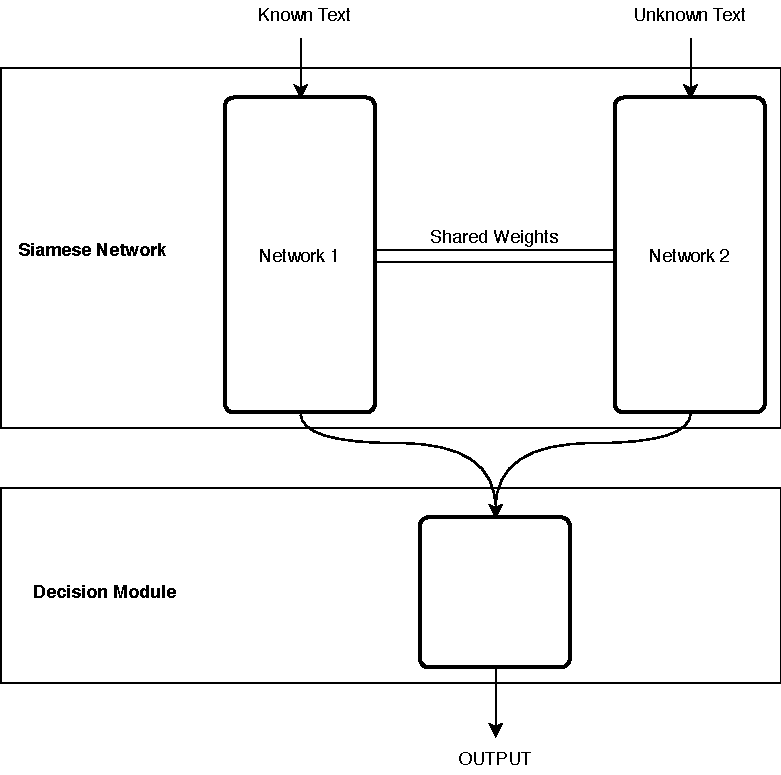
\includegraphics[scale=0.5]{./pictures/method/siamese}
    \caption{The basic architecture of a siamese neural network. The network
        takes two sources of data and runs it through two parallel weight
        sharing networks. The two parallel networks extracts features from the
        raw data. Those features are given to a prediction module that compares
        the feature sets extracted. The decision module can be anything that
        compares two vectors such as a distance function or a dense neural
        network.}
    \label{fig:siamese_example}
\end{figure}

The network will take two inputs, a text $t \in T_\alpha$ and a text $t' \in
T_{\alpha'}$. The network will then try to determine whether $\alpha = \alpha'$
by comparing $t$ and $t'$. The siamese part of the network will extract features
from the texts using convolutions or \gls{RNN} layers. These features will serve
as a \textit{representation} of the texts $t$ and $t'$. This representation will
be given to some dense layers which will learn how to compare the feature sets
extracted.

\citet{DBLP:journals/corr/0001KYS17} presented a comparative study of
\glspl{CNN} and \glspl{RNN} in common \gls{NLP} tasks. They found that
\glspl{RNN} generally performed better in tasks where understanding the whole
text was important while \glspl{CNN} performed better when understanding was
secondary and the goal was mainly about finding key phrases or statistical
information from a text. In authorship verification the understanding of the
text is generally irrelevant since we do not have to say anything about what a
text is about but only whether or not it is written by the same author as some
other text. Furthermore classical authorship verification methods have relied on
statistical information from the texts and not on an actual understanding of the
texts. It is for that reason we start chose to base our initial experiments on
\glspl{CNN}.

The final output of the networks we train will be the probability that $\alpha =
\alpha'$. Since the MaCom dataset consist of multiple texts per author and this
network architecture only compares two texts we define a separate system for
making the final prediction based on all the known texts of an author.


\subsection{Combining Neural Network Output}
\label{subsec:combining_neural_network_output}

In the generic Siamese neural network presented in Section
\ref{subsubsec:siamese_networks} the output of the network is a probability
that two texts are written by the same author. However in the problem we are
trying solve defined in Definition \ref{def:authorship_verification} we take
several texts as input. We therefore need a method of combining the predictions
on multiple texts to a single prediction on a particular problem instance. We
do that using a \textit{prediction system}. We let the generic siamese neural
network described above be known as a \textit{text comparison function} $f \in
\mathcal{F}$.

\begin{definition}[Text Comparison Function]
    \label{def:text_comparison_function}

    Let $\mathcal{F} \colon \mathcal{T} \times \mathcal{T} \rightarrow [0, 1]$
    be any function that compares two texts and outputs the probability that the
    the texts are written by the same author.

\end{definition}

For fixed text comparison function $f$, we now define the \textit{weighted
average based prediction system} $P_w$.

\begin{definition}[Weighted Average Prediction System]
    \label{def:weighted_average_prediction_system}

    Let $w: \mathcal{T} \rightarrow [0, 1]$ be a weight function, such that
    $\forall \alpha \in \mathcal{A}: \sum_{t \in T_\alpha} w(t) = 1$. Then the
    weighted average prediction system is given by,

    \begin{align}
        &P_w \colon \mathcal{A} \times \mathcal{T} \times [0, 1] \rightarrow
            \{0, 1\} \\
        &P_w(\alpha, t, \theta) \mapsto \mathbbm{1}\left[
                \sum_{t' \in T_\alpha} w(t') f(t, t') > \theta
            \right],
    \end{align}

    where $\mathbbm{1}\left[\cdot\right]$ is the indicator function.

\end{definition}

That is, the weighted average prediction system $P_w$ returns 1 if the weighted
average of the probability that $t$ is written by the same author as $t'$ for
each $t' \in T_\alpha$ is greater than the threshold $\theta$ and 0 otherwise.

The $\theta$ parameter in $P_w$ determines when we consider an unknown text
to be written by an author. The $\theta$ parameter can be used to enforce how
sure we have to be of a decision to accuse an author of not having written
an assignment. As described earlier MaCom does not want to accuse innocent
students of cheating. That means that it is very important to MaCom to minimize
the accusation error. We can use the $\theta$ parameter to control that error.
Hopefully the \glspl{FN} will generally end up with a value closer to 1 than
the \glspl{TN}. If that is the case then lowering $\theta$ value will lower the
fraction since there will be fewer \glspl{FN}. That might lower the overall
accuracy of the prediction system but will make sure that at few students as
possible are falsely accused.

The $w$ parameter in the prediction system can be used to weigh the known
texts differently. We are going to try several different weight functions
that weigh texts based on metadata such as the time they were written and the
length of the texts. In the following definition of different weight functions
we will ignore the constraint that the weight functions has to sum to 1 for
each author. We ignore that constraint since for any weight function $w \colon
\mathcal{T} \rightarrow \mathbb{R}$ we can define a new weight function $w^*
\colon \mathcal{T} \rightarrow [0, 1]$ as,

\begin{equation}\label{eq:normalize}
    w^*(t) = \frac{w(t)}{\sum_{t' \in T_\alpha} w(t')}.
\end{equation}

We can therefore define the weight functions $w$ while ignoring the constraint
but use $w^*$ as the actual weight function in the weighted prediction system.

The most obvious weighing scheme is to just use a uniform weighting. That way
we simply take an average of the predictions of our networks over the different
texts an author has written.

\begin{definition}[Uniform Weight]
    \label{def:uniform_weight}

    The uniform weight function is given by,

    \begin{align}
        &u \colon \mathcal{T} \rightarrow \{ 1 \} \\
        &u(t) \mapsto 1.
    \end{align}

\end{definition}

The \textit{uniform weight} function does not use any information we know about
the texts. We define it as a baseline to make sure we do not make any weight
functions that are worse than a simple uniform weighing. Our other weight
functions makes use of metadata we know about the texts. We start by defining a
weight function \textit{exponential dropoff weight} that use the time a text was
turned in to MaCom's servers to weight the texts. We assume that newer texts will
better reflect the current writing style of a student than older texts. Recall
that $\tau$ denotes the function that returns the relative time of a text as
described in Section \ref{subsec:notation}.

\begin{definition}[Exponential Dropoff Weight]
    \label{def:exponential_dropoff_weight}

    Given $\lambda \in \mathbb{R}^+$ the time based exponential dropoff weight
    function is given by,

    \begin{align}
        &exp_\lambda \colon \mathcal{T} \rightarrow \mathbb{R}^+ \\
        &exp_\lambda(t) \mapsto e^{-\lambda \tau(t)}.
    \end{align}

\end{definition}

The $\lambda$ parameter can be used to control how important newer texts are.
When $\lambda = 0$ the exponential dropoff weight is equivalent to the Uniform
Weight function and as $\lambda \rightarrow \infty$ more weight is given to the
most recent text. We have shown the weights given to different assignments for
different $\lambda$ values in Figure \ref{fig:weights}.

\begin{figure}
    \centering
    \textbf{Exponential Dropoff Weights}\par\medskip
    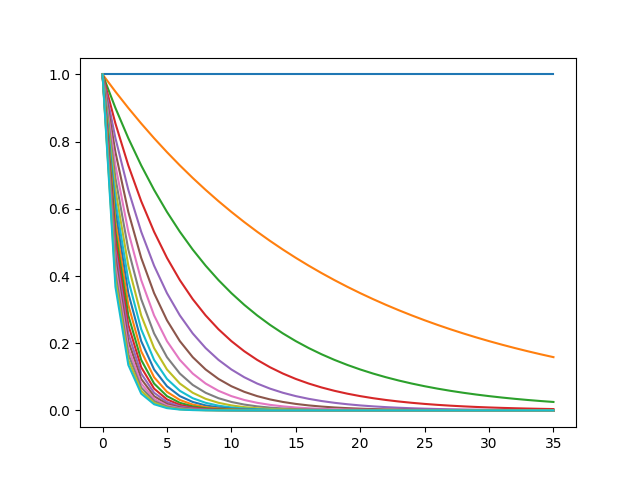
\includegraphics[width=0.49\textwidth]{./pictures/method/weights.png}
    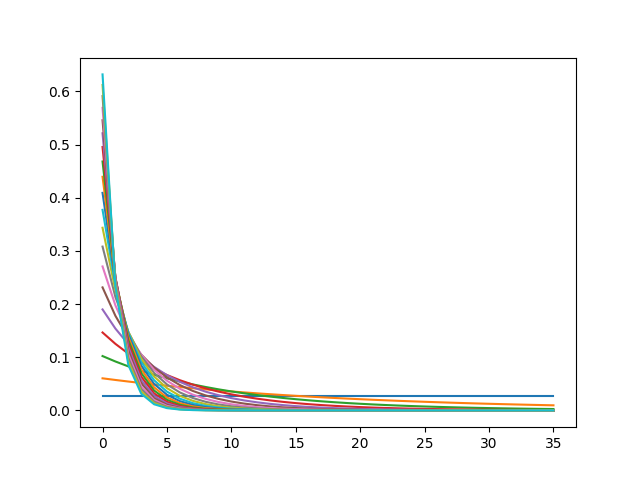
\includegraphics[width=0.49\textwidth]{./pictures/method/weights_normalized.png}
    \caption{Illustrate the exponential dropoff weight function for different
    values of $\lambda$. We apply the weight function to the numbers $0, 1,
    \dots, 35$ since a typical student will attend secondary school for 3 years
    (36 months). On the left the pure output of the weight function $w_e$ is
    shown and on the right the normalized weights $w_e^*$. We wary $\lambda$
    from 0 to 1 with step size 0.05.}
    \label{fig:weights}
\end{figure}

We have also defined weight functions that use other metadata besides the time
of writing. Specifically we have used the length of texts. The idea is that
longer texts provide better insight into an authors writing style than shorter
texts. So we wanted to see if we could obtain better results if we considered
text length.

\begin{definition}[Length Weight]

    The text length based weight function is given by,

    \begin{align}
        &l \colon \mathcal{T} \rightarrow \mathbb{N}^+ \\
        &l(t) \mapsto \left\lfloor \frac{|t|}{1000} \right\rceil + 1,
    \end{align}

    where $\lfloor x \rceil$ is $x$ rounded to nearest whole number.

\end{definition}

Thus this weight function gives more weight the longer a text is but where only
differences on the order of thousands of characters are considered significant.
We used the exponential dropoff weight and length weight functions to implement
another weight function that use both text length and time to give weights to an
assignment. The combined weight function is shown below.

\begin{definition}[Exponential Dropoff and Length Weight]

    Given $\lambda \in \mathbb{R}^+$ the combined time and length weight
    function is given by,

    \begin{align}
        &lexp_\lambda \colon \mathcal{T} \rightarrow [0, 2] \\
        &lexp_\lambda(t) \mapsto exp^*_\lambda(t) + l^*(t).
    \end{align}

\end{definition}

Which is simply the addition of the exponential dropoff weight and the length
weight, after they are both individually applied to the text.

We have also defined some different prediction systems that are not based on
weighted averages. The first such system is the $P_{max}$ prediction system.
The thought behind the system is that we wanted to minimize the accusation
error. The prediction system takes the text $t' \in T_\alpha$ that looks the
most like $t$. That way if just a single assignment from a candidate author
looks sufficiently like the text we are comparing with we report that the author
matches. That should hopefully result in less people being accused of ghost
writing.

\begin{definition}[Maximum Prediction System]
    \label{def:maximum_prediction_system}

    The maximum prediction system $P_{max}$ based only on most similar text is
    given by,

    \begin{align}
        &P_{max} \colon \mathcal{A} \times \mathcal{T} \times [0, 1] \rightarrow
            \{0, 1\} \\
        &P_{max}(\alpha, t, \theta) \mapsto \mathbbm{1}\left[
                \underset{t' \in T_\alpha}{\text{maximize}} f(t, t') > \theta
            \right].
    \end{align}

\end{definition}

For completeness we also defined a $P_{min}$ that use only the least similar
text for the prediction. We expect that such a function will be quick to accuse
authors of ghostwriting since it only looks at the one text that seem to
indicate ghostwriting.

\begin{definition}[Minimum Prediction System]
    \label{def:minimum_prediction_system}

    The minimum prediction system $P_{min}$ based only on least similar text is
    given by,

    \begin{align}
        &P_{min} \colon \mathcal{A} \times \mathcal{T} \times [0, 1] \rightarrow
            \{0, 1\} \\
        &P_{min}(\alpha, t, \theta) \mapsto \mathbbm{1}\left[
                \underset{t' \in T_\alpha}{\text{minimize}} f(t, t') > \theta
            \right].
    \end{align}

\end{definition}

Finally we also defined prediction system that takes a majority vote. The
majority vote is similar to a uniform weight function. The difference is that
the majority vote does not use the actual value of a prediction but only how
many are on each side of a threshold. As an example assume that an author
$\alpha$ has written three texts $\{t_1, t_2, t_3\} = T_\alpha$ and we are
comparing to text $t$ with $\theta = 0.5$. Let us then assume that $f(t, t_1) =
0.0$, $f(t, t_2) = 0.51$ and $f(t, t_3) = 0.51$. Then the uniform weight
function would compute $\mathbbm{1} \left[ \frac{1}{3} 0.0 + \frac{1}{3} 0.51 +
\frac{1}{3} 0.51 > 0.5 \right] = 0$. Meaning that the author would be accused of
using a ghostwriter even though two of his assignments are more similar than
dissimilar. Contrary to that a majority vote would report 1 since more
texts are greater than $\theta$ than lower.

\begin{definition}[Majority Vote Prediction System]
    \label{def:majority_vote_prediction_system}

    The majority vote prediction system $P_{MV}$ is given by,

    \begin{align}
        &P_{MV} \colon \mathcal{A} \times \mathcal{T} \times [0, 1] \rightarrow
            \{0, 1\} \\
        &P_{MV}(\alpha, t, \theta) \mapsto \mathbbm{1}\left[
                \frac{1}{|T_\alpha|} \sum_{t' \in T_\alpha} \mathbbm{1}\left[
                    f(t, t') > \theta
                \right] > \frac{1}{2}
            \right].
    \end{align}

\end{definition}


\subsubsection{Tuning Parameters}
\label{subsubsec:tuning_parameters}

The prediction systems defined above has several hyperparameters we have to
choose to get the best results. We recall that MaCom wanted a system that
had an accusation error of less than 10\%. We can use the shared threshold
parameter $\theta$ in the prediction systems to control how many people we
accuse. The best parameters for the prediction systems is those parameters that
gives the highest accuracy subject to the 10\% accusation error constraint. To
tune the parameters we use a validation dataset not seen during training. From
that dataset we construct a set of tuples $(\alpha, t_u)$ where $\alpha$ is a
candidate author and $t_u$ is a text of unknown authorship. We let the set of
tuples be known as $V$. The parameters that maximize the accuracy subject to the
bounded accusation error is the same as the parameters that minimize the error
rate subject to the bounded accusation error. That optimization problem is,

\begin{equation}
    \label{eq:prediction_system_minimization}
    \begin{aligned}
        & \underset{\theta, x}{\text{minimize}}
        & & \sum_{(\alpha, t_u) \in V} \left|
            P_x(T_\alpha \setminus \{t_u\}, t_u, \theta) -
            \mathbbm{1}\left[t_u \in T_\alpha\right]
        \right| \\
        & \text{subject to}
        & & \frac{\sum_{(\alpha, t_u) \in V} \mathbbm{1}\left[t_u \in T_\alpha\right] \cdot
            \left(1 - P_x(T_\alpha \setminus \{t_u\}, t_u, \theta)\right)}
{\sum_{(\alpha, t_u) \in V} (1 - P_x(T_\alpha \setminus \{t_u\}, t_u, \theta)} <
            \frac{1}{10}
    \end{aligned}
\end{equation}

In the optimization problem we fix the network $f$ like we did when defining
the prediction systems. The expression we minimize is the number of errors made
in prediction over the validation set $V$. Consider a problem $(\alpha, t_u)
\in V$ where $t_u \in T_\alpha$. Then we know that $\mathbbm{1}\left[t_u \in
T_\alpha\right] = 1$ from the definition of the indicator function then if the
prediction system returns the correct result 1 we have,

\begin{equation}
    e = \left|
        P_x(T_\alpha \setminus \{t_u\}, t_u, \theta) -
        \mathbbm{1}\left[t_u \in T_\alpha\right]
    \right| = |1 - 1| = 0,
\end{equation}

and if the prediction system returns the incorrect result 0 we have,

\begin{equation}
    e = \left|
        P_x(T_\alpha \setminus \{t_u\}, t_u, \theta) -
        \mathbbm{1}\left[t_u \in T_\alpha\right]
    \right| = |0 - 1| = 1.
\end{equation}

Similarly for a problem $(\alpha, t_u) \in V$ where $t_u \notin T_\alpha$ we
know that $\mathbbm{1}\left[t_u \in T_\alpha\right] = 0$ from the definition of
the indicator function. Then if the prediction system returns the correct result
0 we have,

\begin{equation}
    e = \left|
        P_x(T_\alpha \setminus \{t_u\}, t_u, \theta) -
        \mathbbm{1}\left[t_u \in T_\alpha\right]
    \right| = |0 - 0| = 0, \end{equation}

and if the prediction system returns the incorrect result 1 we have,

\begin{equation}
    e = \left|
        P_x(T_\alpha \setminus \{t_u\}, t_u, \theta) -
        \mathbbm{1}\left[t_u \in T_\alpha\right]
    \right| = |1 - 0| = 1.
\end{equation}

That is the expression we minimize is 0 whenever there is no error and 1
whenever there is an error. So we minimize the number of errors we make. The
subject to expression makes sure that the fraction of false accusations we make
is less than $10\%$ of the accusations we make. The expression should be read
as,

\begin{equation}
    \frac{\textit{false accusations}}{\textit{total accusations}} < \frac{1}{10}
\end{equation}

Consider the numerator of the fraction on the left hand side,

\begin{equation}
    \textit{false accusations} = \sum_{(\alpha, t_u) \in V}
    \mathbbm{1}\left[t_u \in T_\alpha\right] \cdot
    \left(1 - P_x(T_\alpha \setminus \{t_u\}, t_u, \theta)\right).
\end{equation}

For a $(\alpha, t_u) \in V$ where $t_u \in T_\alpha$ we have that
$\mathbbm{1}\left[t_u \in T_\alpha\right] = 1$ then if $P$ is correct it returns 1 and we
get,

\begin{equation}
    \mathbbm{1}\left[t_u \in T_\alpha\right] \cdot
    \left(1 - P_x(T_\alpha \setminus \{t_u\}, t_u, \theta)\right) =
    1 \cdot (1 - 1) = 0,
\end{equation}

and if $P$ is incorrect and returns 0 we have,

\begin{equation}
    \mathbbm{1}\left[t_u \in T_\alpha\right] \cdot
    \left(1 - P_x(T_\alpha \setminus \{t_u\}, t_u, \theta)\right) =
    1 \cdot (1 - 0) = 1.
\end{equation}

Similarly for a $(\alpha, t_u) \in V$ where $t_u \in T_\alpha$ we have that
$\mathbbm{1}\left[t_u \in T_\alpha\right] = 0$ and therefore the expression is always
0. Therefore the expression is 1 whenever we have a false accusation and 0
otherwise. The right hand side of the inequality simply counts the number of
accusations by inverting the output of $P_x$ and divides that by 10. So the
condition makes sure that only 10\% of the accusations we make are false
accusations.

In the real world it has been estimated that 4\% of turn
ins for the \gls{SRP} are written by "ghostwriters"
\footnote{https://politiken.dk/indland/uddannelse/art5603163/Gymnasieelever-\%C2
\% BBSnyderi-beviser-hvor-vanvittig-betydningsfuld-SRP-er-blevet\%C2\%AB}.
We therefore want to find the best prediction system and threshold $\theta$
on a dataset with 4\% negatives. We also find the best prediction system and
threshold for a dataset with 50\% negatives as that is easier to compare with
other methods.


\subsection{Summary}

To summarize we will implement 2 baseline methods and an indeterminate number of
neural network based methods. The baseline methods will be the extended delta
method and an author specific \gls{SVM} method. The baselines will both need
manually extracted feature sets and feature tuning. The networks will be siamese
neural networks. They work by using either convolutional or recurrent networks
to extract features from raw text data. The features are compared using a dense
network. Each of our neural networks will only compare two texts at a time.
Since an author has multiple texts we will combine the predictions on each of
an author's texts using a prediction system. We will find the best prediction
system and parameters using a validation.

    \FloatBarrier

    \section{Data} \label{sec:data}

As described earlier we use data from the Danish company MaCom. The dataset
provided by MaCom is a file consisting of set of texts in Danish where each text
is associated with an author ID. Throughout the development process we've been
given several data extract. The final extract used for experiments consisted of
a set of 10.250 authors, where a maximum of 100 authors were extracted from each
school. In total, this is 133749 texts. Before running any kind of experiments,
this data was split up into several parts, each part severing a different
purpose in our experimentation. The splitting of the data can be seen in Figure
\ref{fig:data_split}. The purpose of the sets are the following:

\begin{figure}
    \centering
    \textbf{Illustration of Datasets}\par\medskip
    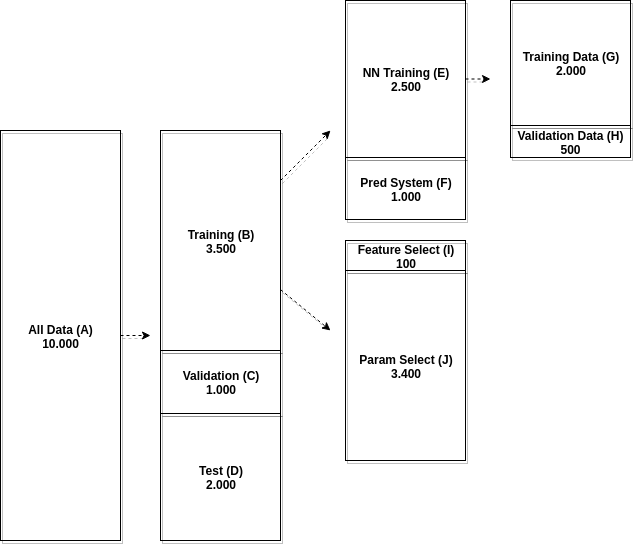
\includegraphics[width=.8\textwidth]{./pictures/data/Data.png}
    \caption{Shows how we have split the dataset we are given. The splits are
        performed on the number of authors in each set. That means that all of
        an authors texts are contained in the same dataset. In particular that
        means that the test dataset contains completely unseen authors that has
        not been used in any training/hyper-parameter selection.}
    \label{fig:data_split}
\end{figure}

\begin{itemize}

    \item[- (A).]

        The entire set of extracted data. This consists of text written by,
        10.058 different danish high school students, spanning different schools
        throughout the country.

    \item[- (B).]

        Consisting of the texts written by 5.500 different authors, this set
        if used in the training process for the \gls{NN}s where it is used for
        training/validation and the prediction system. It is also used for the
        baseline methods, where this entire set is used as the corpus.

    \item[- (C).]

        Being untouched throughout the training process, this set is used for
        unbiased validation, and selection of networks to be used on the test
        set (D). Contrary to the training set (B), this is only used for the
        final selection of our best models during the training process.

    \item[- (D).]

        The test set, which as the name implies, is used to test the performance
        of our final models.

    \item[- (E).]

        As mentioned (B) is used for training both the baselines and the
        \gls{NN}s. In both circumstances, and different split of (B) is
        performed. (E) is the data used for the actual training of the
        \gls{NN}s.

    \item[- (F).]

        This set is used as the basis of the prediction system described in the
        earlier sections of this paper.

    \item[- (G).]

        The training data which is given to our \gls{NN}s.

    \item[- (H).]

        A separate validation set, where no authors overlap with (H), which is
        used to determine the accuracy of our the model on an independent set
        of authors during training. This allows us to stop the training when we
        reach the desired generalization and accuracy.

    \item[- (I).]

        This is an alternate split of (B), used on the baseline methods together
        with set (J). It is used perform the feature selection for both the SVM
        and the Extended Delta method. The specifics of this process will be
        described in Section \ref{subsec:baseline}.

    \item[- (J).]

        This set is used to tune the baseline methods. (J) is used to determine
        the best hyperparameters for the baseline methods. This would be K and
        p in the case of the Extended Delta Method, and C and Gamma for the SVM.
        Like with (I), the specifics of this parameter selection will be covered
        in Section \ref{subsec:baseline}.

\end{itemize}

The training set (B), consists of a total of 73311 texts written in the same
class, split over the 5.500 authors, from different schools. Each authors has
written in average 13 texts, with the standard deviation being 4.2. We initially
removed the first 200 characters of each text, as the beginning of each text
contains a lot of authorship identifying information, such as name, school, and
specifics class. The removal of these characters also make sure that no garbage
texts are included. The texts vary a lot in both structure and length, spanning
from poems to essays. It is for this reason that this sets character count has
a standard deviation of 4133 even though the average character count of 5516.
The full statistics of the training set (B) can be seen in the appendix, Section
\ref{sec:B_stats}.

Due this to this disparity in terms of the contents of the data, some
constraints had to be applied to the data. The reason for this is ,in most
cases, that the non-existence of the constraints would result in either some
computational inefficiency accompanied by a minor increase in data-quality, or
simply just a computational impossibility such as a single text consuming all
memory causing our models to crash. Another purpose of these constraints is to
make the dataset generalize better by removing the outliers.

As can be seen in the statistics in Section \ref{sec:B_stats}, the text
containing the smallest consists of 0 characters, and does obviously not
contain any valuable information. In addition to the 200 characters we removed
initially, we also removed texts that have below 200 characters left after
the removal, as they do not provide enough information about that specific
author, and would work properly with our baseline methods due to the size. The
application of this constraint, resulted in 1.823 of the 73.311 texts being
removed. After which we applied a upper constraint, in terms of the total number
of characters. The reason for this, was a mentioned earlier, that there are some
texts eating up all the available memory, such as the largest text in (B), which
consists of 338.315 characters. We found that limiting the number of characters
to 30.000 gave good results, by removing the crash-inducing texts, without
affecting the overall data-quality too much, as this only removed 119 texts from
(B).

Since we also perform some sentence level networks as well, we also chose to
limit the max number of sentences, for the same reason as with the characters.
The text with the largest amount of sentences, contains 4401 sentences. With
an average sentence count of 49 and a standard deviation of 39, this text is
obviously an outlier, and doesn't generalize the data set very well. A such we
impose a upper limit of 500 sentences per text, which removes another 26 texts
from (B).

The last constraint regards the unique characters in each text. Look at the
stats we can see that there is a text containing 219 unique characters, greatly
exceeding the average of 57. A unique character count like this, implies that a
non-danish alphabet might have been used, and for that reason texts like these
do not add to the generalization we strive towards. This is combatted creating a
list of characters based on the data used for training, each character in this
list is mapped to a replacement character if ever encountered in either the
training or the validation set. The characters are placed in this list if they
occur with a frequency smaller than $10^{-5}$. This threshold was determined
by looking at the danish characters Æ,Ø and Å. In the set (B) they have
a frequency just above $10^{-5}$. We want these included, as we hypothesize
that they generalize danish student well. Additionally we can see in Figure
\ref{fig:character_frequencies}, along with the other thresholds, that after
the character frequency threshold, the overall of frequency of the specific
characters drops dramatically.

After applying all of the constraints, and taking into account overlap between
them, 1.944 texts were removed from the total 73.311 in (B), which is a
negligible amount compared to the computational and generalization advantages it
includes. In the end this leaves set (B) with 71.367 texts.

The aforementioned constraints were not all applied to entirety (A) in the same
manner. Both (C) and (D) are used in a testing context, for that reason removing
the first 200 characters wont make sense as we only did that to prevent the
training process in latching on to author specific meta-data in the text. We
still apply the lower constraint of 200, as this system was intended for usage
of the large SRP assignment the students make at the end of their last year,
this this constraints scrubs away potential garbage texts. The upper limit
is removed, as this was only a step to prevent our methods from crashing. By
applying the methods on a students assignment in a singular fashion rather than
a batch one, we will not have the same problem.

\begin{figure}[htb]
    \begin{minipage}{.5\linewidth}
        \centering
        \subfloat[]{\label{main:a}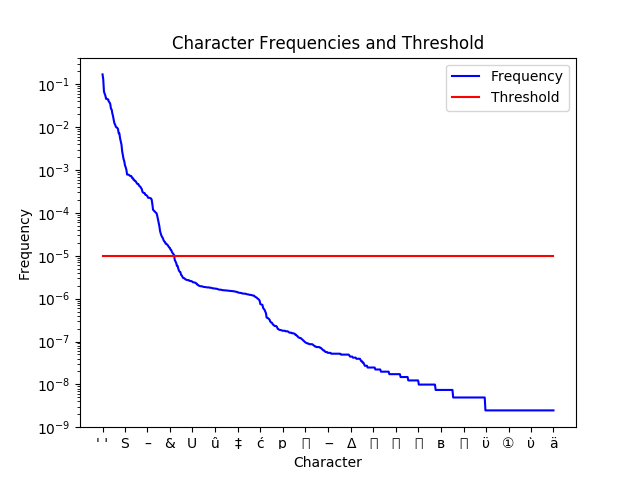
\includegraphics[scale=.5]{./pictures/data/Frequencies.png}}
    \end{minipage}%
    \begin{minipage}{.5\linewidth}
        \centering
        \subfloat[]{\label{main:b}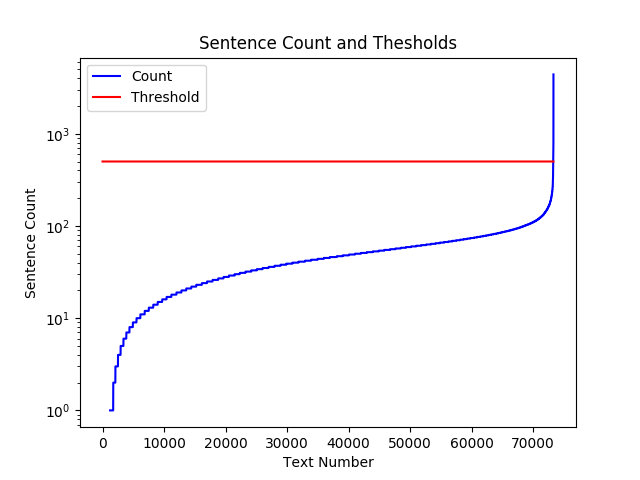
\includegraphics[scale=.5]{./pictures/data/SentenceCount.png}}
    \end{minipage}\par\medskip
    \centering
    \subfloat[]{\label{main:c}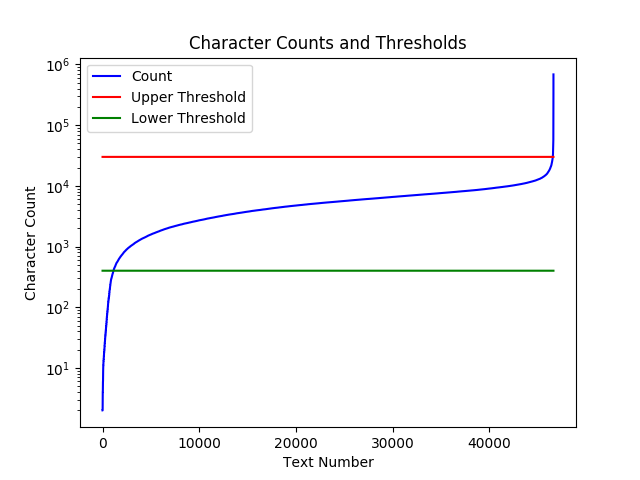
\includegraphics[scale=.5]{./pictures/data/CharacterCount.png}}

    \caption{The different thresholds applied to the during preprocessing.}
    \label{fig:character_frequencies}
\end{figure}

All of the neural networks we train are Siamese Neural Networks. They all
work by comparing two texts at a time. We therefore had to generate problem
instances that contained two texts from either the same or different authors and
a class that reflected that. For each author $\alpha$ in the training dataset
$G$ we generate all possible combinations of two of the texts in $T_\alpha$
as positive samples. We also generate the same number of negative samples by
taking a random text in $T_\alpha$ and a random text in $\overline{T_\alpha}$.
That means that in total the number of problems we generate for each
author is $2\frac{\left|T_\alpha\right|!}{2!(\left|T_\alpha\right|-2)!}
= \frac{\left|T_\alpha\right|!}{(\left|T_\alpha\right|-2)!} =
(\left|T_\alpha\right| - 0) \cdot (\left|T_\alpha\right| - 1) $. The neural
networks are trained on these problem instances. We generate problems in the
same way for the network training validation dataset $H$.

    \FloatBarrier

    \section{Experiments} \label{sec:experiments} 

We have previously described the theory behind the methods we are implementing
to solve the authorship verification problem. In this section we will describe
in detail the experiments we performed to find the optimal hyperparameters and
network structure. We will test each method implemented against the external
validation set \gls{C}.

\subsection{Baseline Methods} \label{subsec:baseline_methods}

The implementation of both the \gls{SVM} and the Extended Delta method closely
resembles the implementation used by \citet{US}. There is however a big
difference with the application of the delta method. Contrary to the scenario
in \citep{US} where PAN data was used there is not an instance where we only
have 1 text per author. Therefore the original version of the delta method can
be used as described by \citet{evert2015towards}. This is the method where when
given a new text $t$ supposedly written by an author $\alpha \in \mathcal{A}$
his texts $T_\alpha$ are extracted and so is a set of texts not written by
him $\hat{T}_\alpha$ where $|\hat{T}_\alpha| = |T_\alpha|$. The text $t$ is
given to a \gls{KNN} classifier which determines if $t \in T_\alpha$ or $t \in
\hat{T}_\alpha$.

% TODO: Consider whether we should move some of the above description to method.


\subsubsection{Feature Selection}

The experiments performed on our baseline methods was centered around parameter
tuning. Not only parameters such as the $K$ in the extended delta method but
also the set of features supplied to the methods. Other methods such as random
forest has a built in filter for bad and noisy features. This is not the case
for both the \gls{SVM} and the extended delta method who does performs any kind
of quality analysis of the feature they are given. It is worst for the extended
delta method as that is just a distance metric that has no way of weighing
features. Therefore we chose to perform a feature selection for them rather than
just having them use the entire set available to them. Contrary to what was done
by \citet{US} this process did not consist of trying out some random selection
of features but rather a more systematic approach was used.

We started by generating a set of features. The feature set is simply a set of
n-grams. In order for us to find as good a feature set as possible we created a
large initial feature set to increase the feature search space. To generate the
features we used a corpus of text. Specifically we used the \gls{B} dataset as a
corpus. From the corpus we enumerated all the different n-grams in the different
categories and computed the frequency of each n-gram. The corpus had,

\begin{itemize}
    \item 27,535 different word-1-grams,
    \item 188,472 different word-2-grams,
    \item 2,178 different character-2-grams,
    \item 219 different \gls{POS}-tag-2-grams, and
    \item 524 special-character-2-grams.
\end{itemize}

The quantities here are large due to the size of the corpus and will continue
to rise as $n$ increases. Rather than extracting all of those features from
our texts we chose to focus on the n-grams with highest frequency as those are
probably the most important features. Specifically consider a case where a very
infrequent feature were chosen. That feature might only exist in the corpus and
in none of the texts in the test set. That feature would therefore be useless
in determining the authorship of those texts. Using the quantities listed above
as inspiration we generated a candidate feature set of 4950 features. The set
consisted of,

\begin{itemize}

    \item

        The frequencies of the 500 most frequent word-n-grams for $n \in \{1, 2,
        3, 4\}$,

    \item

        The frequencies of the 300 most frequent character-n-grams for $n \in
        \{2, 3, ..., 10\}$,

    \item

        The frequencies of the 50 most frequent \gls{POS}-tag-n-grams for $n \in
        \{3, 4\}$, and

    \item

        The frequencies of the 50 most frequent special-character-n-grams for $n
        \in \{2, 3, 4\}$.

\end{itemize}

The quantities extracted reflects the inherent number of different n-grams of
that type. Since there are many more different words than characters there will
also be many more different word-n-grams than character-n-grams of the same
size. We therefore also use more of the most frequent word-n-grams. The sizes
of the different character n-grams we extracted was based on the amount used by
\citet{aalykke2016}. They found that character n-grams of size 8 worked very
well on MaComs data which is the reason why we chose to include char-n-grams
with n spanning the values from 1 to 10. \citet{US} showed that the when $n$
in word-n-grams reach a value of 4, the probability of that sequence actually
occurring in any given text is drastically reduced. A similar thing can be seen
with the special-character-n-grams where an increase in n would not contribute
anything. The reason for the small amount of \gls{POS}-tag-n-grams was that they
were a computationally expensive, as such a reduction in possible n-values had
to be made.

Having the features we could start doing our feature selection. The process
proved very computationally expensive. Having to check every combination of 4950
different features simply was not feasible. Therefore we implemented a greedy
algorithm instead in combination with using only a small dataset \gls{I} for the
feature selection.

The greedy algorithm as described by \citet{kanDeng} is a simple forward feature
selection. Having our previously created feature set we loop through each single
feature validating its accuracy when applied to each $\alpha \in \mathcal{A}$,
where $\mathcal{A}$ is the dataset \gls{I}. The validation on each author
$\alpha$ consists of fetching $T_{\alpha}$ and a set $\hat{T}_{\alpha} \subset
\overline{T}_\alpha$, where $|\hat{T}_\alpha| = |T_\alpha|$. Using these sets
of positive and negative cases we use k-fold cross validation to determine
the performance of the feature for that author $\alpha$. This is done for all
authors and when averaged we have the performance of that single feature. This
process is then repeated for all features. The best performing feature is then
added to a set of candidate features. In the next iteration we loop through all
the features again but we validate against each feature in combination with
the already selected features. This process is repeated until a set number of
features are selected. At that point the feature set that generated the highest
score is chosen.

Due to the increased run-time when using leave one out cross validation we had
to make use of some other model selection approach. Under normal circumstances
normal X-fold cross validation would work out fine but a complication arose when
doing this with the extended delta method. The reason for this was that there
was a scenario where an unlucky split of folds would cause a lot of error. A
generic example of this would be if we had a 2 class training set consisting
of 6 values evenly split between the 2 classes. In the case where we split
those 6 values into 3 folds there is a chance that a fold contains two values
of the same class which means that if $K = 3$ both of those wont ever be able
to classified correctly as there is only 1 of that class in the training set.
As such, stratified K fold cross validation is used instead as it uphold the
class distribution in its folds. While this is not a proglem for the \gls{SVM}
classifier we also opted the stratified K fold cross so we would more directly
compare the feature selection of the two models.

For both the \gls{SVM} and dxtended delta method, we ran this algorithm
until 450 features were selected. The \gls{SVM} performed its feature selection
using the default RBF kernel, a C with value of 1, and $\gamma =
\frac{1}{\text{n\_features}}$. Due to some authors having below 3 texts,
the default K value of \glspl{KNN} K parameter was set to 3 for the feature
selection.

The results of both the \gls{SVM} and the extended delta method feature selection can
be seen in Figure \ref{fig:fs_results}. The best number of selected feature were
220 for the SVM and 4 for the extended delta Method, scoring an accuracy of
0.697 and 0.672 respectively.

\begin{figure}
    \centering
    \textbf{Greedy Feature Selection}\par\medskip
    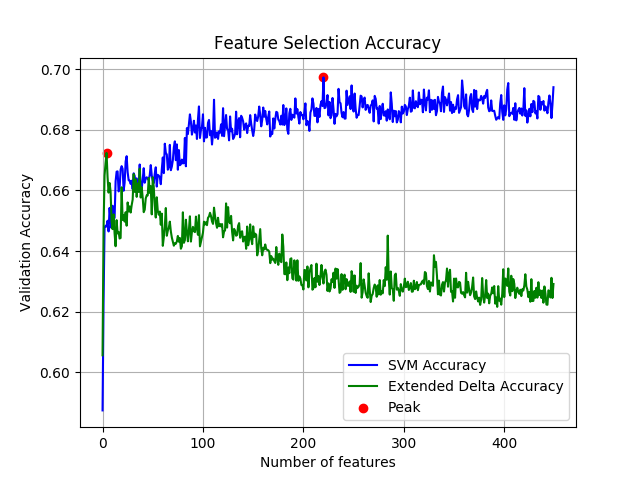
\includegraphics[scale=0.6]{./pictures/experiments/feature_selection}
    \caption{The process of the greedy feature selection of the SVM and the
        extended delta Method. The x axis shows the number of selected features
        so far in the search and the y axis the average accuracy when using that
        feature set for each author. The extended delta method peaks with a very
        small feature set while the \gls{SVM} needed more features to maximize
        accuracy.
    }
    \label{fig:fs_results}
\end{figure}


\subsubsection{Hyper Parameter Selection}\label{sec:hyp_select}

As mentioned in the previous section due to time constraints we were unable
to do the hyper parameter selection in parallel with the feature selection.
For that reason we chose to split it up selecting our features first and then
tuning the parameters based on those selected features. As before where we
searched for features in a set of features we now search for parameters in a set
of parameters. Recall that the \gls{SVM} need the $C$ and $\gamma$ parameters
and the extended delta method need the $p$ and $K$ parameters. We search for
parameters in a grid search of the values,

\begin{align}
    \text{SVM} &:
    \begin{array}{lr}
        C=\{10^{-3}, 10^{-1}, 10^{1}, 10^{3}, 10^{5}, 10^7\}\\
        \gamma=\{10^{-3}, 10^{-1}, 10^{1}, 10^{3}, 10^{5}, 10^7\}
    \end{array} \\
    \text{Extended Delta} &:
    \begin{array}{lr}
        p=\{1,2,3,4,5\}\\
        K=\{1,3,5,7,9,11,13,15\}
    \end{array}.
\end{align}

For each variation of the hyper parameters we average the performance of the
method over all unique authors in the training set in a manner very similar
to the feature selection. We make use of the same 3-fold stratified cross
validation and arrange each author with set of opposing set of texts. The
accuracy of each parameter configuration can be seen in Table \ref{table:KNN}
for the extended delta method, and Table \ref{table:SVM} for the \gls{SVM}. The
parameter search was performed on the \gls{J} dataset.

\begin{table}[h]
    \centering
    \textbf{\gls{KNN} Cross Validation Results}\par\medskip
    \begin{tabular}{|c|ccccc|}
        \hline
        \backslashbox{$K$}{$p$} & 1 & 2 & 3 & 4 & 5 \\\hline
        1 & \textbf{0.630} & 0.603 & 0.588 & 0.577 & 0.570\\
        3 & 0.628 & 0.589 & 0.572 & 0.565 & 0.555 \\
        5 & 0.621 & 0.576 & 0.559 & 0.549 & 0.545 \\
        7 & 0.612 & 0.564 & 0.546 & 0.537 & 0.533 \\
        9 & 0.600 & 0.554 & 0.537 & 0.527 & 0.524 \\
        11 & 0.587 & 0.542 & 0.527 & 0.520 & 0.517 \\
        13 & 0.581 & 0.537 & 0.524 & 0.517 & 0.514 \\
        15 & 0.571 & 0.532 & 0.519 & 0.514 & 0.512 \\\hline
    \end{tabular}
    \caption{The results from performing a grid search of the $p$ and $K$
        parameters of the \gls{KNN} algorithm.}
    \label{table:KNN}
\end{table}

\begin{table}[h]
    \centering
    \textbf{\gls{SVM} Cross Validation Results}\par\medskip
    \begin{tabular}{|c|cccccc|}
        \hline
        \backslashbox{$C$}{$\gamma$} & $10^{-3}$ & $10^{-1}$ & $10^{1}$ & $10^{3}$ & $10^{5}$ & $10^{7}$ \\\hline
         $10^{-3}$ & 0.626 & 0.626 & 0.626 & 0.641 & 0.558 & 0.500 \\
         $10^{-1}$ & 0.626 & 0.626 & 0.626 & 0.641 & 0.558 & 0.500 \\
         $10^{1}$  & 0.626 & 0.626 & 0.626 & \textbf{0.689} & 0.576 & 0.501 \\
         $10^{3}$  & 0.626 & 0.626 & 0.681 & 0.687 & 0.576 & 0.501 \\
         $10^{5}$  & 0.626 & 0.680 & 0.678 & 0.687 & 0.576 & 0.501 \\
         $10^{7}$  & 0.674 & 0.678 & 0.678 & 0.687 & 0.576 & 0.501 \\\hline
    \end{tabular}
    \caption{The results from performing a grid search for $C$ and $\gamma$ of
        the \gls{SVM} algorithm}
    \label{table:SVM}
\end{table}

We performed a validation of the methods on the \gls{C} dataset. While
applying these methods to a validation set wont change anything in terms of
the parameters we have selected. It will give us the ability to gauge the
accuracy of our methods when applied to a new never before seen test-set.
Using this untouched data set as the base the validation determines what text
from each author is the newest one ending up with a set of samples of the
form $(t, \alpha)$ where $t$ is a text and $\alpha$ is an author. For each
of these samples $T'_\alpha = T_\alpha \setminus \{t\}$ is extracted from
\gls{C}. Additionally another randomly sampled set $\hat{T}_\alpha \subset
\overline{T}_\alpha$ is extracted where $|\hat{T}_\alpha| = |T'_\alpha|$. Using
the combined set $T'_\alpha \cup \hat{T}_\alpha$, we can train the model in
question having provided it with both positive and negative examples of author
$\alpha$ writing style. To include samples that depict a student that used a
ghost writer we change the text we do our prediction on. For each sample there
is a probability that the sample will be regarded as negative. If that is the
case we pick out a random $t'$ where $t' \in (\overline{T}_\alpha \setminus
\hat{T}_\alpha)$ and predict on that where a correct prediction would be the
model say he did not write it. In the positive case we simply predict on $t$ and
a correct prediction would be the model saying he did write it. The results of
this process can be seen in Table \ref{tab:baseline-val-res}.

\begin{table}[h]
    \centering
    \begin{tabular}{|c|c|c|c|c|c|c||c|c|}
        \hline
        Split & Classifier & Params & TP & TN & FP & FN & \textbf{Accuracy} & \textbf{Accu Err} \\ \hline
        \multirow{2}{*}{50/50} & SVM & \{C:10, $\gamma$:1000\} &  759 & 692 & 308 & 241 & \textbf{0.7255} & \textbf{0.2583} \\ \cline{2-9} 
        & ED & \{K:1, p:1\} & 667 & 583 & 417 & 333 & \textbf{0.625} & \textbf{0.36353} \\ \hline
        \multirow{2}{*}{96/04} & SVM & \{C:10, $\gamma$:1000\} & 762 & 23 & 25 & 238 & \textbf{0.749} & \textbf{0.91187} \\ \cline{2-9} 
        & ED & \{K:1, p:1\} & 680 & 23 & 23 & 320 & \textbf{0.67208} & \textbf{0.93294} \\ \hline
    \end{tabular}
    \caption{The results of running our two baseline methods the \gls{SVM} and
        Extended Delta method, on the dataset \gls{C} the validation set.}
    \label{tab:baseline-val-res}
\end{table}

Unfortunately both of these methods are not suitable for the prediction system
described earlier and thus a to get it below the allowed accusation error was
not possible. While this is not ideal for comparative purposes it does lend
credence to the applicability of neural networks to this specific scenario.


\subsection{Deep Learning}

In the prediction system from Definition
\ref{def:weighted_average_prediction_system} we needed a function $f$ that
takes two texts and returns the probability that those texts are written
by the same author. As described earlier siamese \gls{NN}s are well
suited for comparing objects. In this Section we describe the experiments
we performed with different networks architectures and we will present
three different networks. The three networks are \gls{conv-char-NN} in
Section \ref{subsubsec:conv_char_nn}, \gls{conv-char-word-NN} in Section
\ref{subsubsec:conv_char_word_nn}, and \gls{rec-sent-NN} in Section
\ref{subsubsec:rec_sent_nn}.

The data we trained our networks on is described in Section \ref{sec:data}. We
trained the networks on the \gls{G} dataset that contains 3,000 authors. We used
early stopping based on a validation dataset \gls{H} that contains 500 authors.
Through experimentation we found that the validation dataset had to contain
completely different authors than the training dataset. In the beginning of
our project we had a validation set that contained different problem instances
(two texts to compare) from the training set but contained some of the same
authors. That lead to the validation set not being a very good estimate of the
networks performance on different authors than the ones seen during training.
The networks were therefore overfitting on the specific authors and we could not
see that in the validation datasets accuracy. All accuracy graphs shown in this
Section are based on a validation dataset with 500 completely unseen authors.

The general structure of our networks will be that they take two texts as input.
The texts are first embedded into a format that can be used by the network.
Then the texts are transformed into two sets of features representing the text
via a weight sharing network. Then the text representation will be combined
in some way and a dense network will take the combined representations and
decide whether or not the texts are written by the same author. We call the
different parts of the network \textit{Embedding}, \textit{Feature Extraction},
\textit{Combining} and \textit{Decision}.

When we show graphs of the networks we have produced we use specific names for
different layers in the networks. A glossary of the layer names and parameters
of the layers are shown in Table \ref{tab:glossary}.

\begin{landscape}
    \begin{table}
        \centering
        \textbf{Glossary}\par\medskip
        \begin{tabular}{|L{3cm}|L{9cm}|L{11cm}|}
            \hline
            \multicolumn{1}{|c|}{\textbf{Layer}}                               &
            \multicolumn{1}{|c|}{\textbf{Description}}                         &
            \multicolumn{1}{|c|}{\textbf{Actively Used Parameters}}           \\
            \hline

            Input                                                              &
            Serves as the entrypoint of the network, by receiving a set of
            texts and feeding it trough the network.                           &
            \begin{minipage}[t]{\linewidth}
            \begin{compactdesc}
                \item[Shape] The dimensions of each sample give to the input.
            \end{compactdesc}
            \end{minipage}                                                    \\
            \hline

            Embedding                                                          &
            Taking in an encoded sample, it produces a dense vector
            representation for each different. More details can be found in
            Section \ref{subsubsec:layers}.                                    &
            \begin{minipage}[t]{\linewidth}
            \begin{compactdesc}
                \item[Input Dim] Size of vocabulary.
                \item[Output Dim] Size of vector used to represent embedding.
            \end{compactdesc}
            \end{minipage}                                                    \\
            \hline

            Convolutional                                                      &
            Applies convolution to the data it recieves according to the
            decription, found in Section \ref{subsubsec:layers}.               &
            \begin{minipage}[t]{\linewidth}
            \begin{compactdesc}
                \item[Filters] Dimensionality of the output, ie. number of
                    filter from the convolution.
                \item[Kernel Size] Integer or list describing size of
                    convolution window.
                \item[Strides] Stride length of the convolutional window.
                \item[Activation] The activation function to be applied after
                    the convolution.
            \end{compactdesc}
            \end{minipage}                                                    \\
            \hline

            Global Max Pooling                                                 &
            Extracts the maximum value from each of the provided data          &
            No parameters.                                                    \\
            \hline

            Concatenation                                                      &
            As the name suggests, this layers simply concatenates the data it
            receives from different layers                                     &
            No parameters.                                                    \\
            \hline

            Merge                                                              &
            Merges its inputs, using a specified function to generate a single
            output.                                                            &
            \begin{minipage}[t]{\linewidth}
            \begin{compactdesc}
                \item[Function] The function used to merge the recieved data.
            \end{compactdesc}
            \end{minipage}                                                    \\
            \hline

            Dense                                                              &
            A simple fully connected layer, taking in data and applying the
            function described in Section \ref{sec:neurons}.                   &
            \begin{minipage}[t]{\linewidth}
            \begin{compactdesc}
                \item[Units] Number of neurons in in the layer.
                \item[Activation] The activation function to be applied.
            \end{compactdesc}
            \end{minipage}                                                    \\
            \hline

            Dropout                                                            &
            Drops a fraction it receives, with the goal of preventing
            overfitting.                                                       &
            \begin{minipage}[t]{\linewidth}
            \begin{compactdesc}
                \item[Rate] The fraction of data it receives dropped.
            \end{compactdesc}
            \end{minipage}                                                    \\
            \hline

            Lambda                                                             &
            Applies a specified function to the input it receives              &
            \begin{minipage}[t]{\linewidth}
            \begin{compactdesc}
                \item[Function] The function applied.
            \end{compactdesc}
            \end{minipage}                                                    \\
            \hline

            Reshape                                                            &
            Reshapes the data it receives.                                     &
            \begin{minipage}[t]{\linewidth}
            \begin{compactdesc}
                \item[Dim] Dimensionality to reshape to.
            \end{compactdesc}
            \end{minipage}                                                    \\
            \hline

            LSTM                                                               &
            A Long Short-Term Memory layer, which works according to the
            description in Section \ref{subsubsec:layers} is applied to the
            given data.                                                        &
            \begin{minipage}[t]{\linewidth}
            \begin{compactdesc}
                \item[Unit] Number of neurons in the layer.
            \end{compactdesc}
            \end{minipage}                                                    \\
            \hline
        \end{tabular}
        \caption{Glossary used when performing experiments, and creating their
            associated models \citep{chollet2015keras}.}
        \label{tab:glossary}
    \end{table}
\end{landscape}


\subsubsection{\glsdesc{conv-char-NN}}
\label{subsubsec:conv_char_nn}

The idea behind network \gls{conv-char-NN} is that we wanted to use convolutions
to look for n-grams in texts. Traditional authorship verification/attribution
is based on carefully engineered n-grams that are compared between two texts
\citep{stamatos2009}. Instead of choosing the n-grams ourselves we wanted the
network to learn which features are important for the authorship verification
task. The features are learned through convolutions. The convolutions look
at some number of characters at a time and gives a single output for those
characters. Assume for example that the network has learned that the character
sequence "ould " is important for deciding the author of a text. Then we
expect the network to react strongly to character sequences that looks
like "ould ". We have illustrated such a convolutional filter in Figure
\ref{fig:convolution_text_example}.

\begin{figure}
    \centering
    \textbf{Convolutions for Text Feature Extraction}\par\medskip
    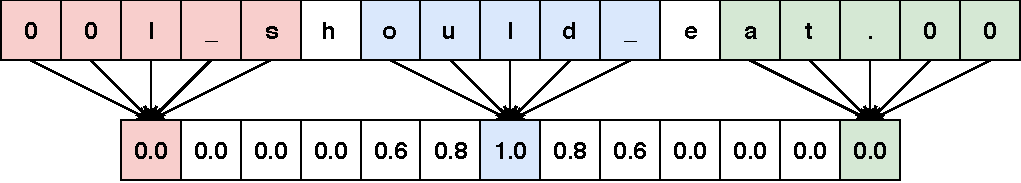
\includegraphics[width=\textwidth]{./pictures/experiments/convolution_example}
    \caption{Illustration of character level convolutions using a filter that
        looks for the character sequence "ould ". Notice that high values are
        produced when the characters the filter looks at match the characters it
        is looking for and low values are produced otherwise. We have
        illustrated 3 different filter locations but the filter is similarly
        placed in all possible locations. We have padded the text with zeros to
        get the same size output as input.}
    \label{fig:convolution_text_example}
\end{figure}

\begin{description}

    \item[Embedding:]

        The embedding takes as input a sequence of integers. Each different
        integer is a compact one-hot encoding of each character. The one-hot
        encoded character stream is embedded in a five dimensional space. The
        hope is that the layer will learn that similar characters should be
        placed close to each other in the output space and dissimilar characters
        should be placed far apart. The same embedding is performed on both of
        the input texts and the layer is therefore part of the siamese part of
        the network.

    \item[Feature Extraction:]

        Features are extracted from the two texts via a layer of convolutions
        with different sizes. We use both convolutions with a window size of
        8 and convolutions with a window size of 4. We use 700 of size 8 and
        500 of size 4. We used a window size of 8 since \citet{aalykke2016}
        found that n-grams of size 8 worked the best for Danish texts and we
        also added 4 so the network could look at smaller n-grams as well.
        We used a stride of 1 such that each convolutional filter could
        observe all parts of the texts and give an output for each one. The
        convolutional part of the network also shares weights such that the
        same features are extracted from both the input texts. We use the
        \gls{ReLu} activation function for the reasons described in Section
        \ref{subsubsec:activation_functions}.

        After the convolutional layer we added a global max pooling layer. The
        layer takes the maximum output of each convolutional filter. We do that
        as the output size of the convolutional layer depends on the length of
        the input text. The output of the max pooling layer is $700 + 500 =
        1200$ numbers, one for each convolutional filter. That means that the
        network learns to extract 1200 different features from each text.

    \item[Combining:]

        The features of the texts are combined using the absolute difference
        function. As described each text is represented as a vector of 1200
        features and to combine them we subtract them from each other and take
        the elementwise absolute difference.

    \item[Decision:]

        The decision part of the network consists of 4 dense layers each with
        500 neurons, a dropout layer and an output layer. The 4 dense layers
        also use the \gls{ReLu} activation function. The dropout layer is added
        just before the output layer and performs 30\% dropout to try to combat
        overfitting. The actual prediction is performed in the output layer.
        The output layer use the softmax function to return a probability
        distribution over the two possibilities that the texts are written by
        the same author and that they are written by different authors.

\end{description}

We have shown an illustration of the network in Figure \ref{fig:conv-char-NN}.
In the Figure we have illustrated the siamese part of the network as a blue box.
The 4 phases of the network is not illustrated in the Figure but it should be
possible to find them by reading the description above. We trained the network
on the dataset described in the Section \ref{sec:data} and in the beginning
of this Section. We used the \gls{Adam} optimizer during the training of the
network. We used a learning rate of $\eta = 0.0005$, half of what was suggested
by \citet{DBLP:journals/corr/KingmaB14}. We did that as we had problems with
neurons dying during the training of the network. Other than the learning rate
we used the parameters suggested in the article. That is, the remembering rates
were set to $\gamma_1 = 0.9$ and $\gamma_2 = 0.999$. As the error function we
used the binary cross-entropy function whose definition can be seen in Lemma
\eqref{eq:binary_ce}.

\begin{figure}
    \centering
    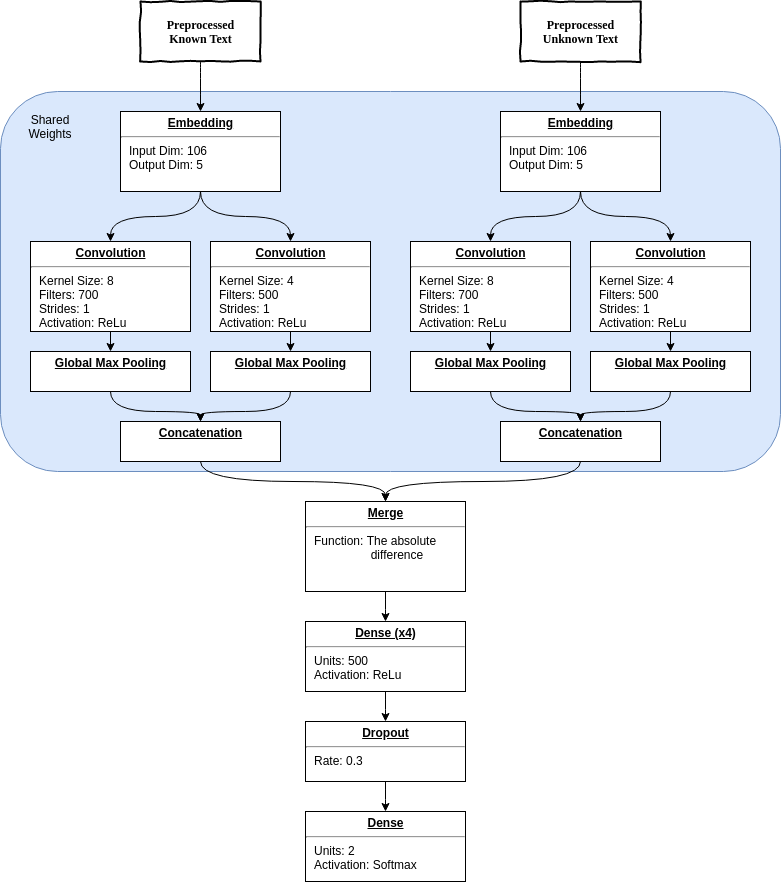
\includegraphics[width=\textwidth]{./pictures/experiments/conv_char_nn/model}
    \caption{The structure of network \gls{conv-char-NN}. Weights are
        shared by the embedding layers and the convolutional layers as shown by
        the blue box. The input to the network is at the top and the output is
        at the bottom. Information flows downwards through the layers. The final
        softmax layer produces a probability distribution over the two
        possibilities that the texts are either written by the same author or
        not.}
    \label{fig:conv-char-NN}
\end{figure}

\begin{lemma}[Binary Cross-Entropy]

    Let the loss function binary cross entropy be defined as,

    \begin{equation}\label{eq:binary_ce}
        L(y, p) = -(y \cdot \log(p) + (1- y)\cdot\log(1 - p)),
    \end{equation}

    where $y : \{0,1\}$ is a label and $p \in [0,1]$ is a predicted probability.

\end{lemma}

When we trained the network we were able to obtain a validation accuracy of
0.71773 in epoch 5. The training accuracy continued rising but we used early
stopping since the validation accuracy had stopped improving. We have shown
a graph of the training and validation accuracies during training in Figure
\ref{fig:conv-char-NN-accuracies}. During the training we used minibatch
learning with a minibatch size of 8. We used a size of 8 as that was the largest
batch size that could fit in the GPUs memory. During the training we padded
all texts with zeros such that all texts in each batch had the same length. We
did that as it is required by keras. We have shown the training and validation
accuracies during training in Figure \ref{fig:conv-char-NN-accuracies}.

\begin{figure}
    \centering
    \textbf{Training and Validation Accuracies for Network \gls{conv-char-NN}}\par\medskip
    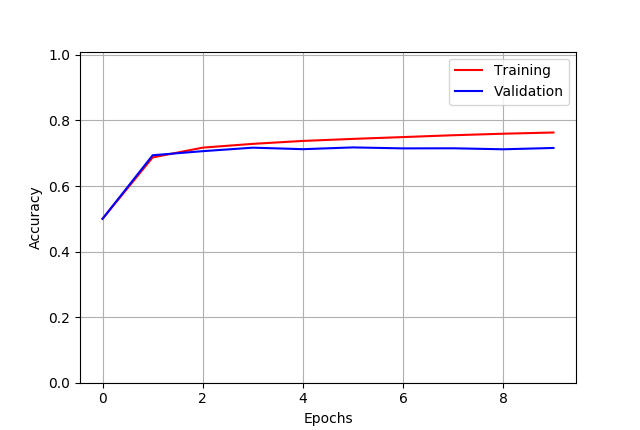
\includegraphics[width=0.5\textwidth]{./pictures/experiments/conv_char_nn/training_accuracy}
    \caption{The training and validation accuracy of \gls{conv-char-NN} during
        training. Each epoch contains several thousand minibatches which is why
        the training and validation accuracies rises so much in the first
        epoch.}
    \label{fig:conv-char-NN-accuracies}
\end{figure}

To arrive at the network architecture described above we experimented with
several similar architectures. We started with a network that was not too
far from the final one. All the work computed in this network was applied
to the same one-hot encoded character level as the final network was. The
feature extraction layer was however quite different. It made use of a single
convolutional layer consisting of 1000 filters with a window size of 10 the
selection of which did not have any proper argument and was selected solely
to determine the initial performance on the data. In addition to that the
combination part of the network also differed. Rather than computing the
absolute difference as was done in the final network, this initial network
simply concatenated the two siamese branches. If we let $t_f = \{t_1, t_2,
\dots, t_n\}$ be the extracted features of the text $t$, then the concatenation
would be computed by,

\begin{equation}
    combine(t, t') \mapsto (t_1, t_2, \dots, t_n, t'_1, t'_2, \dots t'_n)
\end{equation}

Finally the decision part of the network simply consisted of a single 500 neuron
dense network. The network gave promising results which is why we continued
working with it but it quickly overfitted on the training data so we added some
dropout. Like in the network presented above we added the dropout layer just
before the output layer and used 30\% dropout. That regularization allowed the
training accuracy and validation accuracy to follow each other for more epochs
making the final validation accuracy better.

We changed the combining function from a concatenation to a absolute difference
since the network would then not have to learn which features belonged to other
features. The new combination function is computed as,

\begin{equation}\label{eq:abs}
    combine(t, t') \mapsto \left(
        |t_0 - t'_0|, |t_1 - t'_1|, \dots, |t_n - t'_n|
    \right)^T.
\end{equation}

We also tried other combining functions such as the cosine difference but we
did not get any better results. After that change we changed the convolutional
filters from using 1000 filters of size 10 to using 500 filters of size 8 and
500 of size 4. We used those window sizes for the reasons described above. At
the same time we added more dense layers to the model. We again observed the
validation accuracy increasing further. Since our architecture seemed to work
well we scaled up the size of the network to having 4 dense layers instead of 1
as in the final network.

After expanding the network we wanted to figure out which features the network
were looking at. Since the convolutional layer (feature extractor) is followed
by a global max pool we knew that the feature a specific filter was looking
at could be determined by finding the maximum activation of that filter.
Unfortunately we found that the network were looking at metadata about the
texts. Specifically the network were looking at names and school class numbers.
Obviously a real ghost writer would make sure that the correct name and school
class were written on the assignment so in the real world those features should
not be used. The features are a product of the creation of the dataset we are
training on. Since different students assignments are combined to create the
negative samples we are training on (almost) all negative samples will have
different names written in them. Similarly (almost) all negative samples will
have different school classes written on them. Therefore such metadata will be
great features in our training dataset but not necessarily great features in
the real world. In Table \ref{tab:name_features} we have shown the activation
strings of the convolutional filter looking at Danish names.

\begin{table}
    \begin{tabular}{ll}
        \textbf{Activation String} & \textbf{Danish Surnames Matching} \\
        \hline
        \verb!adsen\n\n\n! & Madsen. \\
        \verb!ndsen\n\n\n! & Svendsen, Frandsen. \\
        \verb!elsen\n\n\n! & Nielsen, Mikkelsen. \\
        \verb!ersen\n\n\n! & Pedersen, Andersen, Petersen, Iversen, Jespersen. \\
        \verb!ansen\n\n\n! & Hansen, Christiansen, Johansen, Kristiansen. \\
        \verb!ensen\n\n\n! & Jensen, Christensen, S\o rensen, J\o rgensen,
                             Kristensen, Mortensen, Mogensen. \\
        \verb!arsen\n\n\n! & Larsen. \\
        \verb!ulsen\n\n\n! & Poulsen.
    \end{tabular}
    \caption{Showing the mapping from a convolutional filter looking at endings
        of common Danish surnames and the actual surnames. We found the list of
        the most common Danish surnames at \url{https://bit.ly/1d5WUmT}}
    \label{tab:name_features}
\end{table}

As described in Section \ref{sec:data} we tried to remove as much personal
information as possible from the texts by removing the first 200 characters and
by deleting names from the texts. When we trained the network again with those
preprocessing steps we got a substantial hit in network performance. However the
network were hopefully not looking at metadata anymore.

As described in Section \ref{subsubsec:tuning_parameters} we also have to choose
the best prediction system and best threshold $\theta$ for the network. The
dataset we use to tune the prediction system $P_x$ and threshold $\theta$ are
the \gls{F} dataset. The set consists of 2,000 previously unseen authors. We
find parameters for two cases. One where we generate 50\% positive problems and
50\% negative problems and one where we generate 96\% positive problems and 4\%
negative problems. In the 50/50 case we end up with 4,000 differeent problems.
For each of the authors we generate a positive sample by taking the newest text
as the unknown text and a negative sample by choosing a random text from some
other author in the set.

As described in Section \ref{subsubsec:tuning_parameters} the best threshold
for a prediction system is found by taking the threshold that maximizes
accuracy while having an accusation error of less than 10\%. The best
prediction system is then the system that has the highest accuracy for
their best threshold. We try 1,001 different thresholds $\theta = 0.000,
0.001, \dots, 1.000$ and we try the weight functions $P_\mathcal{U}$,
$P_{exp_{0.25}}$, $P_{exp_{0.50}}$, $P_{exp_{0.75}}$, $P_{exp_{1.00}}$,
$P_{lexp_{0.25}}$, $P_{MV}$, $P_{max}$, $P_{min}$ and $P_l$. We have shown
the accuracy and accusation error for the dataset containing 50\% negatives
in Figure \ref{fig:conv-char-NN-pred-50} and for the dataset containing 4\%
negatives in Figure \ref{fig:conv-char-NN-pred-4}.

\begin{figure}
    \centering
    \textbf{Prediction System Results for 0.5 Split, \gls{conv-char-NN}}\par\medskip
    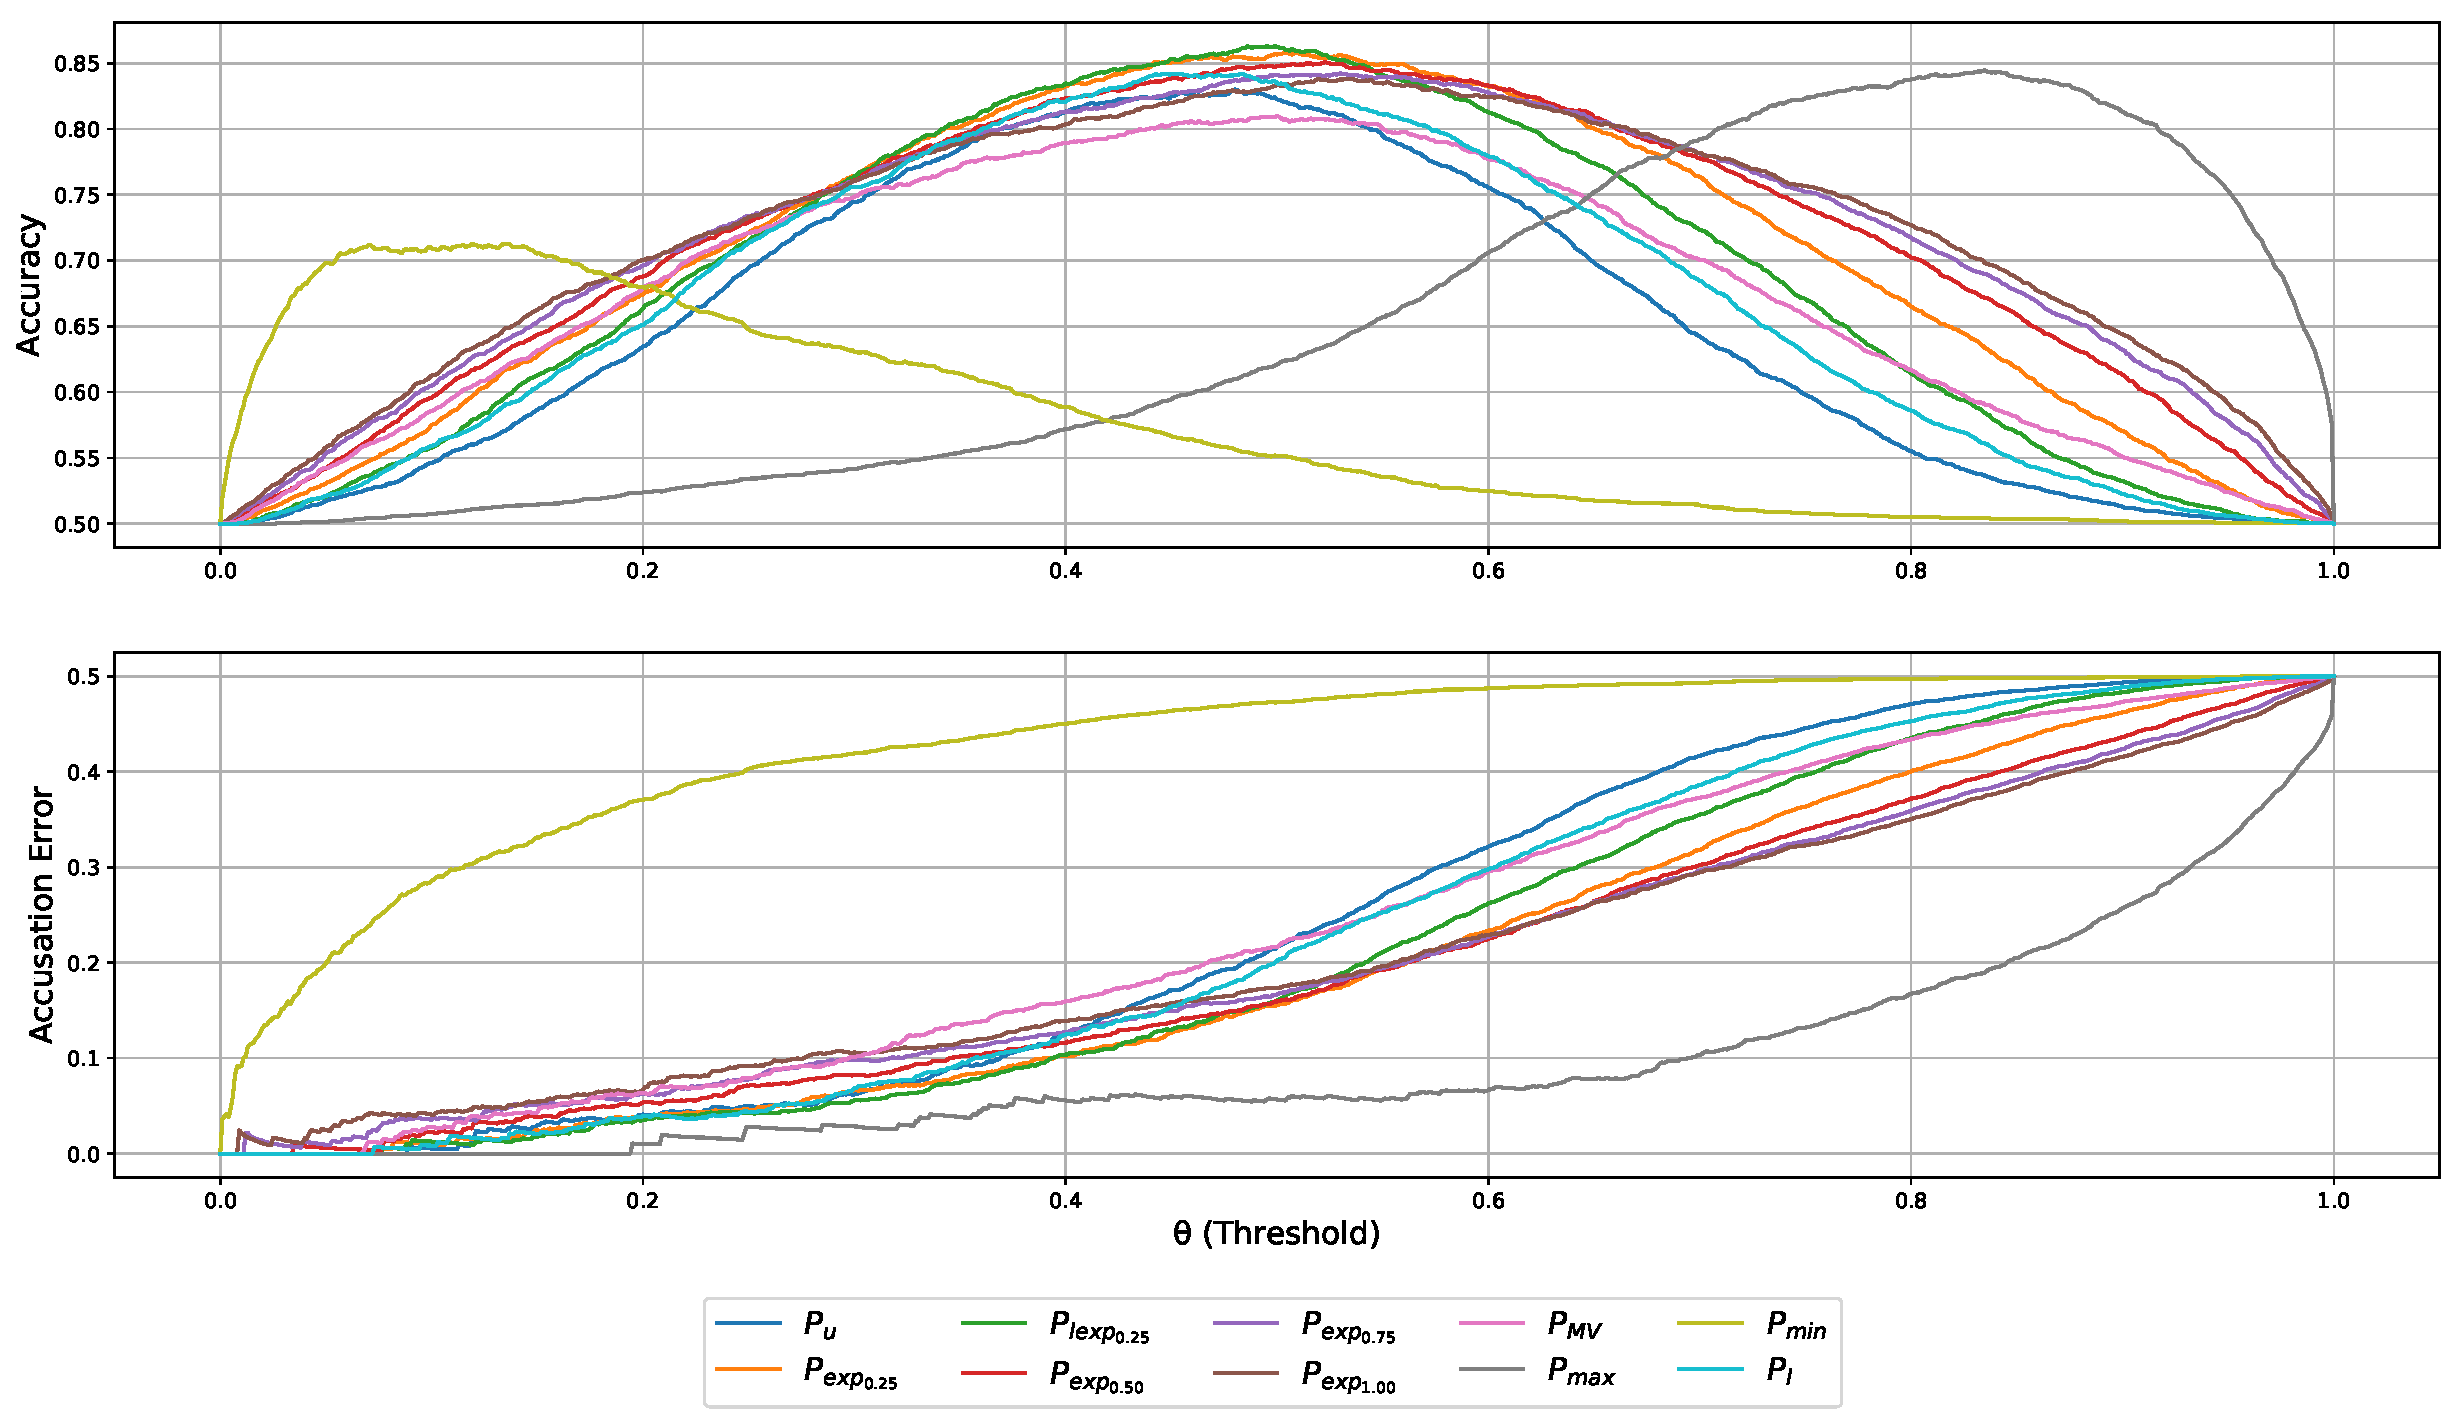
\includegraphics[scale=0.33]{./pictures/experiments/conv_char_nn/prediction_system_50}
    \caption{Results of running the prediction system with the
        \gls{conv-char-NN} on a validation dataset with 50\% positive samples
        and 50\% negative samples. In the upper graph we show the accuracies
        obtained as a function of $\theta$ for different prediction systems
        $P_x$. At the bottom we have shown the accusation error as a function
        $\theta$ again with one line for each prediction system. We can see that
        as the threshold increases and we accuse more people of cheating the
        accusation error rises.}
    \label{fig:conv-char-NN-pred-50}
\end{figure}

\begin{figure}
    \centering
    \textbf{Prediction System Results for 0.04 Split, \gls{conv-char-NN}}\par\medskip
    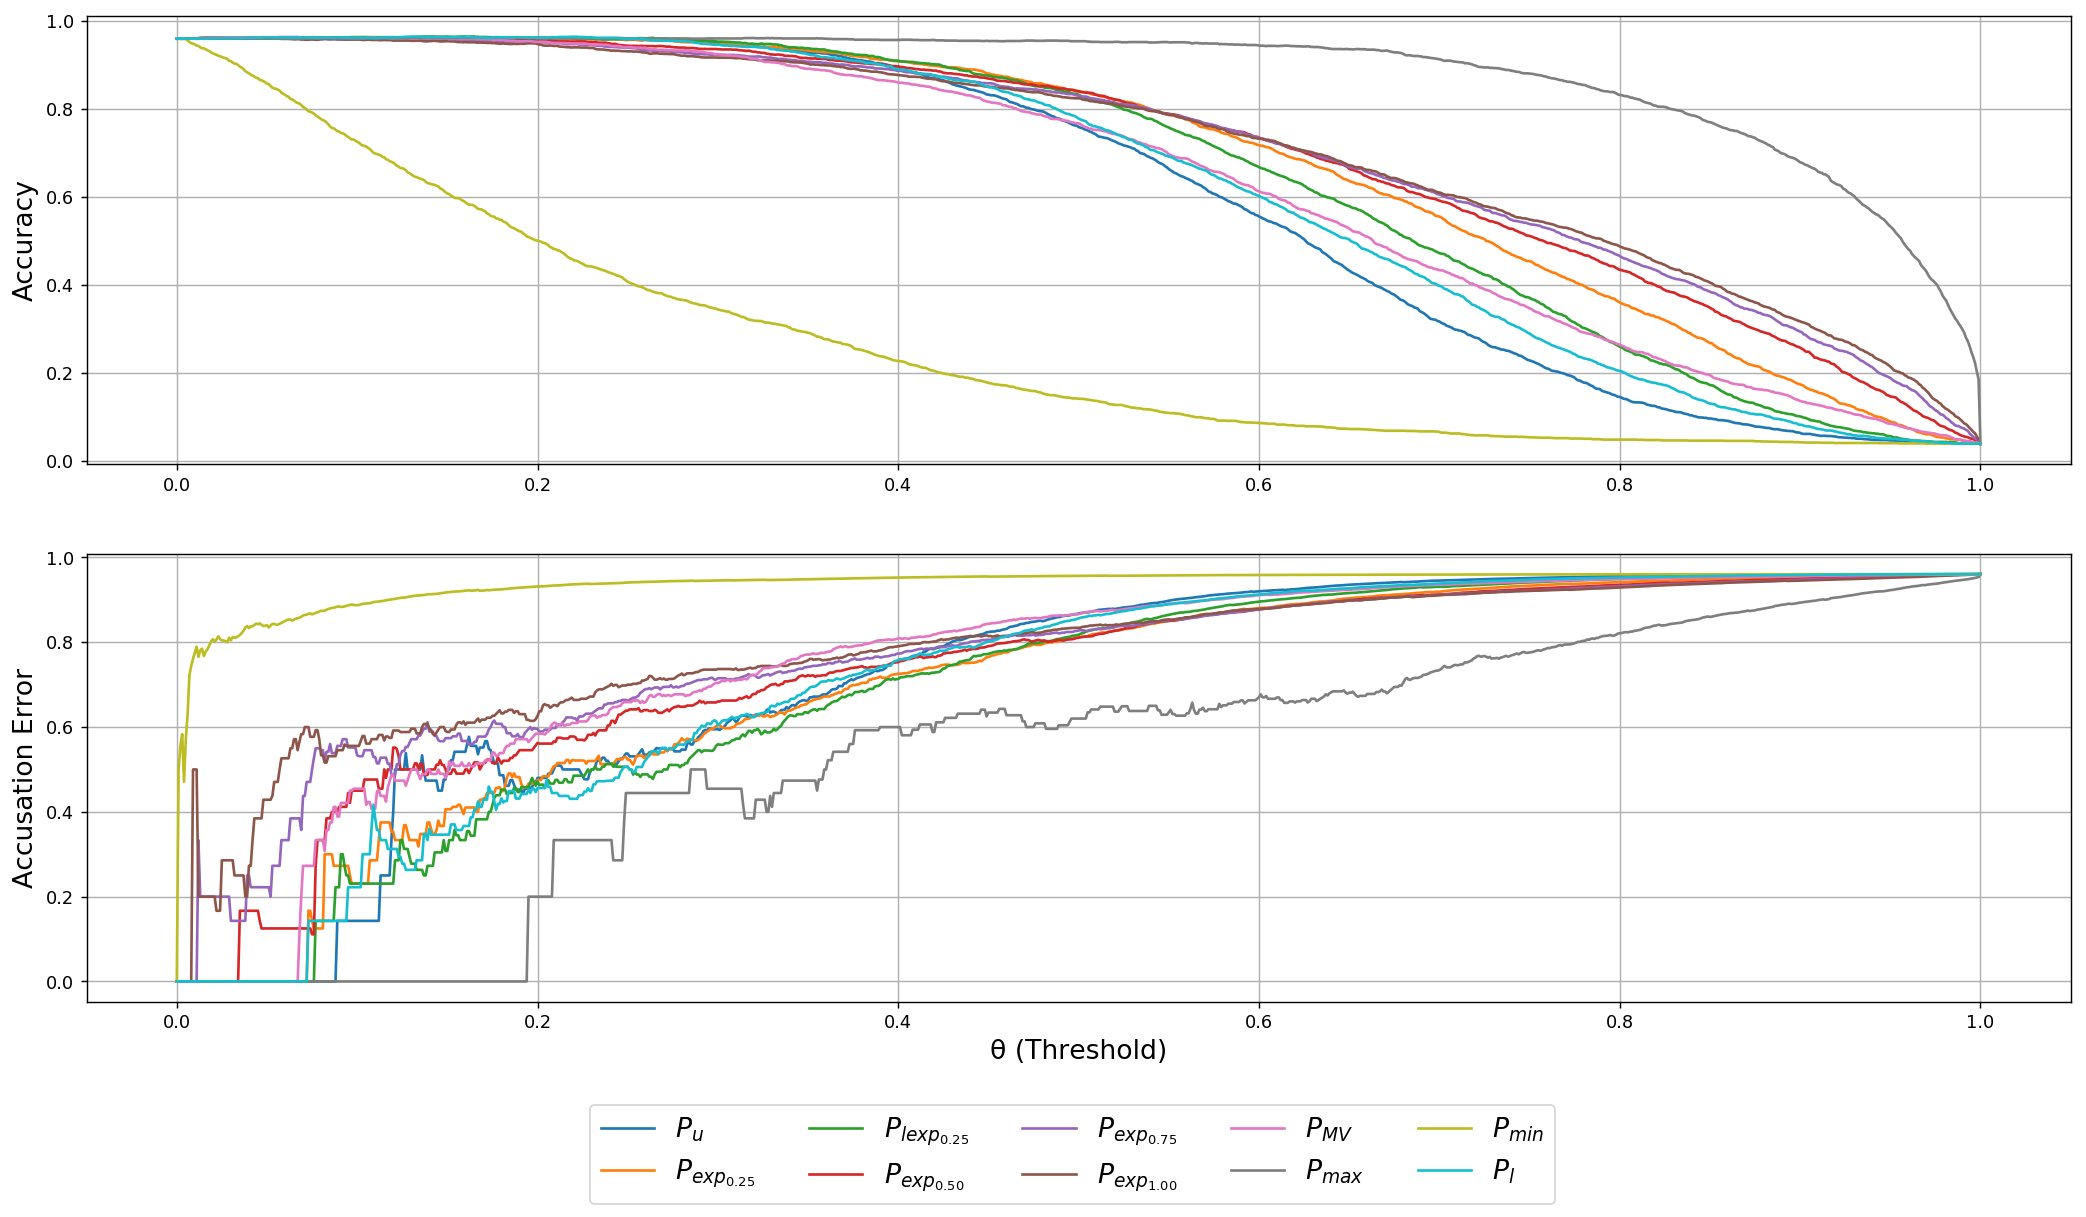
\includegraphics[scale=0.33]{./pictures/experiments/conv_char_nn/prediction_system_04}
    \caption{Results of running the prediction system with \gls{conv-char-NN}
        on a validation dataset with 96\% positive samples and 4\% negative
        samples. In the upper graph we show the accuracies obtained as a
        function of $\theta$ for different prediction systems $P_x$. At the
        bottom we have shown the accusation error as a function $\theta$ again
        with one line for each prediction system. We can see that as the
        threshold increases and we accuse more people of cheating the accusation
        error rises.}
    \label{fig:conv-char-NN-pred-4}
\end{figure}

The best configuration for both the 50/50 split and 96/04 split was the
following,

\begin{center}
\begin{tabular}{|c|c|c|c|c|c|c|c|c|}
\hline
Split & Weight            & $\theta$ & TP  & TN  & FP & FN & Acc    & A-Error \\ \hline
50/50 & $P_{lexp_{0.25}}$ & 0.390    & 1843 & 1482 & 517 & 156 & 0.8316 & 0.095   \\ \hline
96/04 & $P_{mv}$          & 0.057    & 1999 & 8    & 74  & 0   & 0.9644 & 0.000   \\ \hline
\end{tabular}
\end{center}


\subsubsection{\glsdesc{rec-sent-NN}}
\label{subsubsec:rec_sent_nn}

After having attempted a convolutional approach as was just described we
proceeded with some recurrent experiments as well. After having looked at
previous experiments described by \cite{qian:2018} which showed promise in
terms of authorship attribution we considered this a natural extension of
our convolutional approaches. Every \gls{RNN} experiment was performed on
the same data as the convolutional networks and the \textit{Embedding},
\textit{Feature Extraction}, \textit{Combining} and \textit{Comparing} structure
was used as well. The best model we generated can be seen depicted in Figure
\ref{fig:rec-sent-NN}. After 10 epochs this network peaked with a validation
accuracy of 0.657. We have shown a plot of the training and validation
accuracies during training in Figure \ref{fig:rec-sent-NN-training}.

\begin{figure}
    \centering
    \textbf{Training and Validation Accuracies for Network \gls{rec-sent-NN}}\par\medskip
    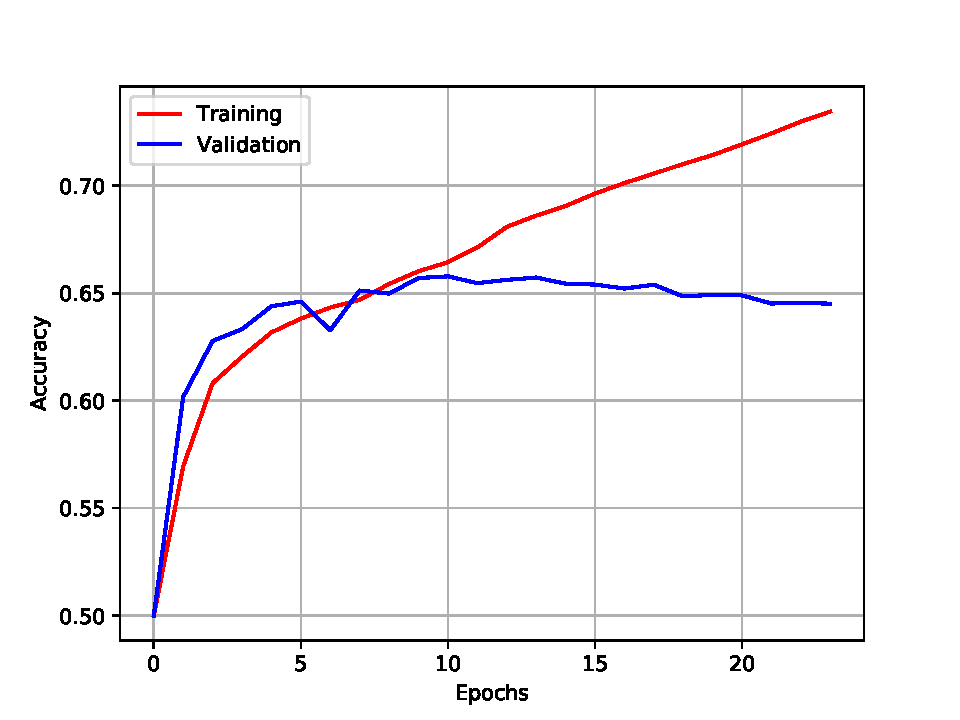
\includegraphics[width=0.5\textwidth]{./pictures/experiments/rec_sent_nn/training}
    \caption{Shows the training and validation accuracies during training of
        \gls{rec-sent-NN}. We stopped training after we observed that the
        validation accuracy no longer followed the training accuracy.}
    \label{fig:rec-sent-NN-training}
\end{figure}

\begin{description}

    \item[Embedding:]

        Like with the previous networks, this network is also a siamese neural
        network. It takes two texts as input and outputs the probability that
        they are written by the same author. As the title of this section
        suggests the network works on the sentence level rather than the
        character level. That clearly has consequences for the embedding part of
        the network.

        The input to the network is given as a sequence of sequences. The outer
        sequence consisting of sentences and the inner sequence consisting
        of the words in each sentence. In order for the dimensionality to
        work the amount of word in a sequence is padded or truncated such
        that they consist of 25 words each. An amount which was chosen based
        on the analysis of the training dataset \gls{B}. Contrary to earlier
        networks the embedded representations of these words were not trained
        as as part of the network. Pre-trained embedding produced by Facebook
        \footnote{\url{https://github.com/facebookresearch/fastText/blob
        /master/ pretrained-vectors.md}} using the method described by
        \citet{bojanowski2016enriching} was used instead. That resulted in each
        word being mapped to a 300 dimensional vector. At this point we have
        a sequence of sentences each containing a sequence of 300 dimensional
        word-embeddings. The network then proceeds to take the average of the
        word sequence contained within each sentence, resulting in each sentence
        being represented as the average of its words.

    \item[Feature Extraction:]

        The feature extraction part of this network consisted of recurrent
        layers. Specifically we used \gls{LSTM} layers described in
        Section \ref{layer:LSTM}. Two \glspl{LSTM} are placed right after
        one another. Both of them consists of 50 units and has the flag
        \textit{return\_sequences} set to true. This results in the output
        of all time-steps of the \gls{LSTM} being returned rather than just
        the last one giving us a sequence of outputs. We then proceed to
        combine all the returned sequences using a global average pooling
        layer. Rather than using a simple \gls{ReLu} which was the activation
        function we used on most layers for the reason explained in Section
        \ref{subsubsec:activation_functions} the \gls{LSTM} use 2 other
        activation functions. It use the tahn activation function from Equation
        \eqref{eq:tanh} after the last time step and the hard sigmoid activation
        function from Equation \eqref{eq:h_sig} after each individual time-step.
        This configuration is the default of the \gls{LSTM} layer provided by
        keras making the only change to the default parameters the number of
        units in the layer.

        The idea behind this feature extraction network was that we would
        extract 50 features from each sentence. We would then take the average
        over the whole text to extract 50 features that represented the author.
        Those features will then be used to combine the two texts. The feature
        extraction approach is very similar to what is done by
        \citet{qian:2018} who got very good results.

    \item[Combining:]

        Like the networks described in the earlier sections the combinations
        of our two siamese paths are done by taking the absolute difference
        of their two max-pooling outputs.

    \item[Decision:]

        The decision part of this network was kept quite simple. It simply
        consists of a single dense layer of 100 units which is then followed
        by a 30\% dropout layer for regularization. The result of the dropout
        layer is then provided to the last dense layer of 2 neurons using
        the soft-max activation function thus mapping it into a probability
        distribution. Since two neurons were used to depict the final output
        the loss function used for the network was binary cross-entropy paired
        with a \gls{Adam} optimizer with the learning rate of 0.0005, 50\% of
        the default value.

\end{description}

\begin{figure}
    \centering
    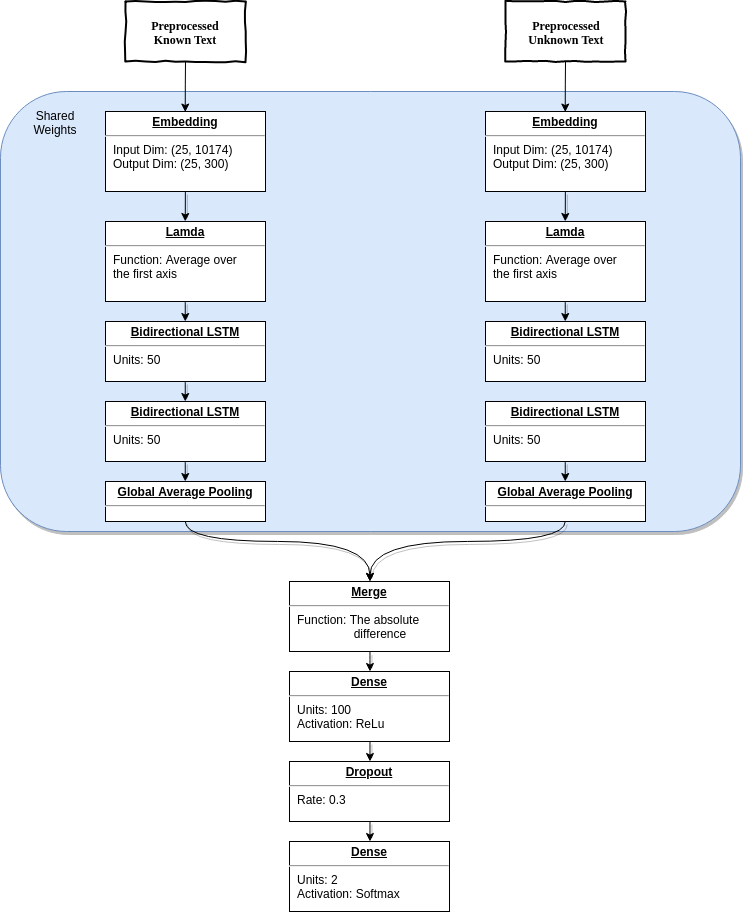
\includegraphics[width=\textwidth]{./pictures/experiments/rec_sent_nn/model}
    \caption{The structure of network \gls{rec-sent-NN}. The weights are shared
        from from the embedding layer all the way down to right before the two
        paths merge. The lambda layer takes each sentence and averages along
        the first axis causing the dimensionality to change from a matrix with
        25 rows and 300 columns to a column vector with 300 elements. The LSTM
        layers are bidirectional meaning its runs through the layer from both
        directions resulting in an output dimensionality twice the unit count
        of 50.
    \label{fig:rec-sent-NN}}
\end{figure}

The path to this final design was a long one. The initial network designs
for our recurrent networks was based on a combination of the work done by
\citet{qian:2018} and our \gls{conv-char-NN} network described in Section
\ref{subsubsec:conv_char_nn}. We simply replaced the feature extraction
component in the network from convolutional layers to recurrent layers. In
addition that the first \gls{RNN} network also used the cosine similarity as its
method of combination on decision. It was when running this network, that the
main hindrance when using a character level recurrent network became apparent,
computation time. This first iteration of the network needed an estimated 140
hours to run through a single epoch. That was a very long time to train a
network and it was not feasible for us to try that in our limited time.

An attempt at saving training time was the inclusion of a convolutional layer
in the feature extraction part of the network. This would be placed before the
recurrent layers in an attempt to minimize the amount of data that was given to
the recurrent layers. The convolution used a window size of 8 and a stride of 8
meaning that each text would be 8 times smaller after the convolutional layer.
This did decrease the runtime but only resulted in an accuracy of 0.532 at its
peak. This was slightly increased when replacing the cosine similarity with a
series of dense layers instead and using a bidirectional \gls{LSTM} layer rather
than a single \gls{GRU} layer.

Instead of using convolutions to limit the text size we also tried changing
the linguistic level our network worked at. Again inspired by \cite{qian:2018}
we elevated our network from using the characters of the texts to using the
sentences. This sentence representation was achieved by doing as was described
in the \textbf{Embedding} part above. This approach significantly decreased
the runtime to around $1.5$ hours. But it also revealed the reason why a
recurrent network might not be the best choice for a task like this. The
validation error throughout training the network was not very high compared to
our earlier convolutional networks. The training accuracy also increased much
more than for the convolutional networks while the validation accuracy quickly
stalled. It therefore seemed like this approach was very prone to overfitting on
particular authors. This lead to the final network described above. This network
included an extra bidirectional \gls{LSTM} layer, and the 0.3 dropout for extra
generalization.

We also chose the best prediction system $P_x$ and best threshold $\theta$ for
this network. We tried the same thresholds and prediction systems as before.
The results can be seen in the Figures, \ref{fig:rec-sent-NN-pred-50} and
\ref{fig:rec-sent-NN-pred-4}

\begin{figure}
    \centering
    \textbf{Prediction System Results for 0.5 Split, \gls{rec-sent-NN}}\par\medskip
    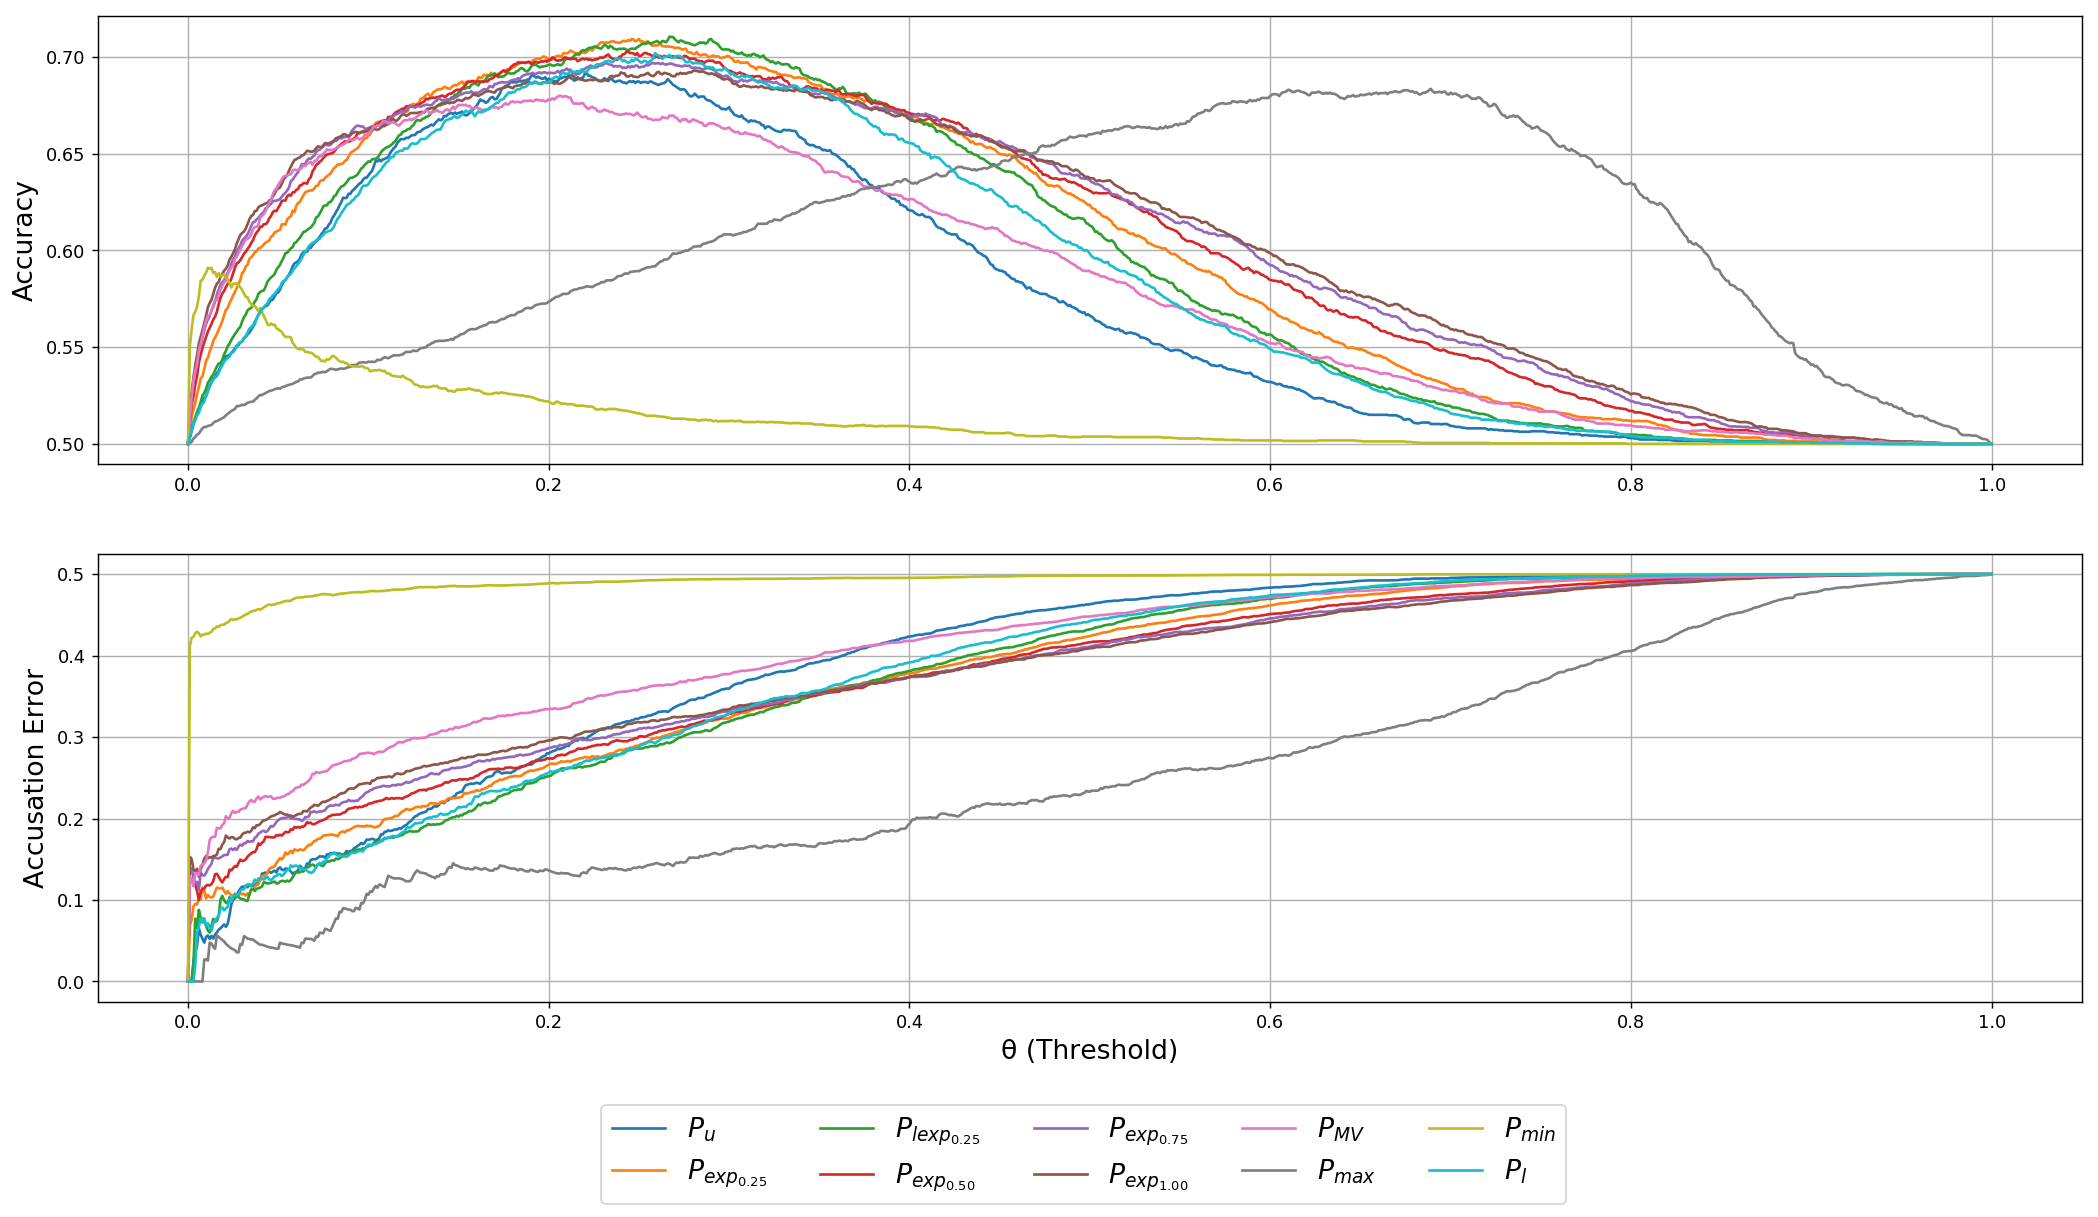
\includegraphics[scale=0.33]{./pictures/experiments/rec_sent_nn/prediction_system_50}
    \caption{Results of running the prediction system with \gls{rec-sent-NN} on
        a validation dataset with 50\% positive samples and 50\% negative
        samples. In the upper graph we show the accuracies obtained as a
        function of $\theta$ for different prediction systems. At the bottom we
        have shown the accusation error as a function $\theta$ again with one
        line for each prediction system. We can see that as the threshold
        increases and we accuse more people of cheating the accusation error
        rises.}
    \label{fig:rec-sent-NN-pred-50}
\end{figure}

\begin{figure}
    \centering
    \textbf{Prediction System Results for 0.04 Split, \gls{rec-sent-NN}}\par\medskip
    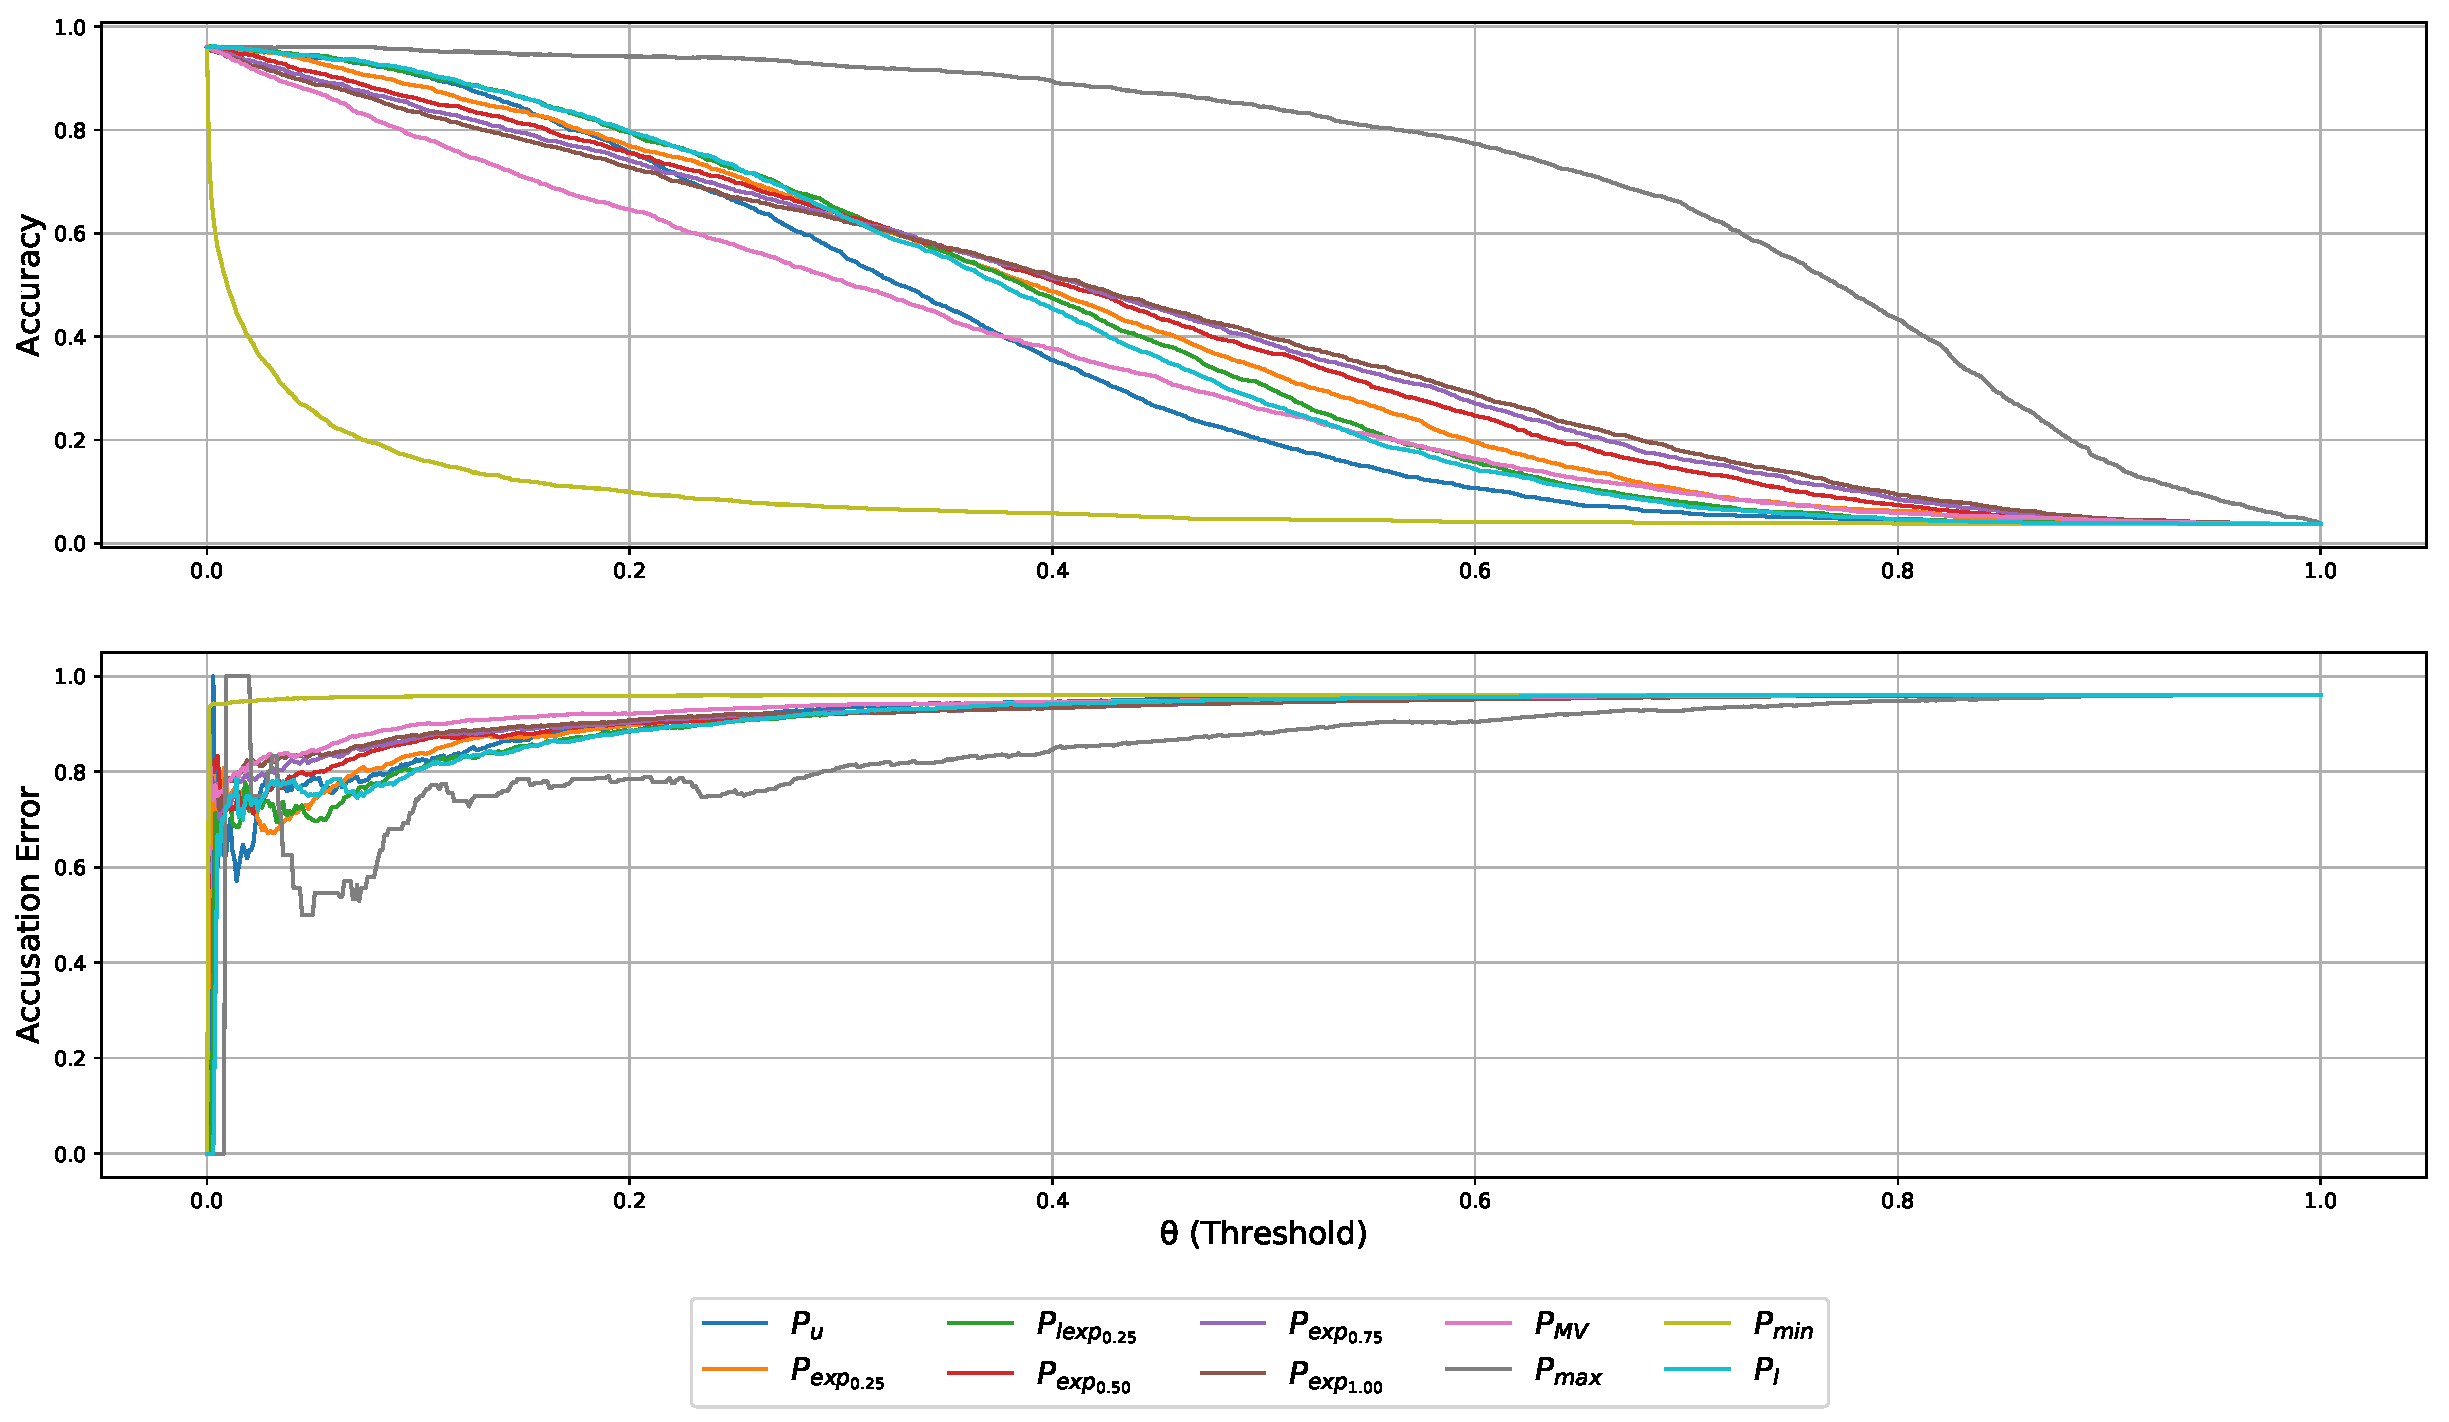
\includegraphics[scale=0.33]{./pictures/experiments/rec_sent_nn/prediction_system_04}
    \caption{Results of running the prediction system with \gls{rec-sent-NN} on
        a validation dataset with 96\% positive samples and 4\% negative
        samples. In the upper graph we show the accuracies obtained as a
        function of $\theta$ for different prediction systems. At the bottom we
        have shown the accusation error as a function $\theta$ again with one
        line for each weight. We can see that as the threshold increases and we
        accuse more people of cheating the accusation error rises.}
    \label{fig:rec-sent-NN-pred-4}
\end{figure}

The best configurations for \gls{rec-sent-NN}, using both the 50/50 and
96/04 split of data was the following,

\begin{center}
    \begin{tabular}{|c|c|c|c|c|c|c|c|c|}
    \hline
    Split & Weight            & $\theta$ & TP   & TN  & FP   & FN  & Acc    & A-Error \\ \hline
    50/50 & $P_{lexp_{0.25}}$ & 0.033    & 1965 & 310 & 1689 & 34  & 0.5690 & 0.099   \\ \hline
    96/04 & $P_{lexp_{0.25}}$ & 0.002    & 1999 & 1   & 79   & 0   & 0.9620 & 0.000   \\ \hline
    \end{tabular}
\end{center}

These result are to expected when looking at the graphs. The immediate spike in
accusation error leaves the model very little room to increase the accuracy in.
This is most likely the result of the aforementioned author specific learning
the network does.


\subsubsection{\glsdesc{conv-char-word-NN}}
\label{subsubsec:conv_char_word_nn}

The last network we produced, is what we call \gls{conv-char-word-NN}. This
network is similar to \gls{conv-char-NN} mostly due being convolutional.
This network was an attempt at expanding on the successful architecture of
\gls{conv-char-NN}. Applied to the same data as the previous networks, we got a
maximum accuracy of 0.697 on the second epoch. We have shown the training and
validation accuracies in Figure \ref{fig:conv-char-word-NN-training}. The design
of the network in the different parts was as follows,

\begin{figure}
    \centering
    \textbf{Training and Validation Accuracies for Network \gls{conv-char-word-NN}}\par\medskip
    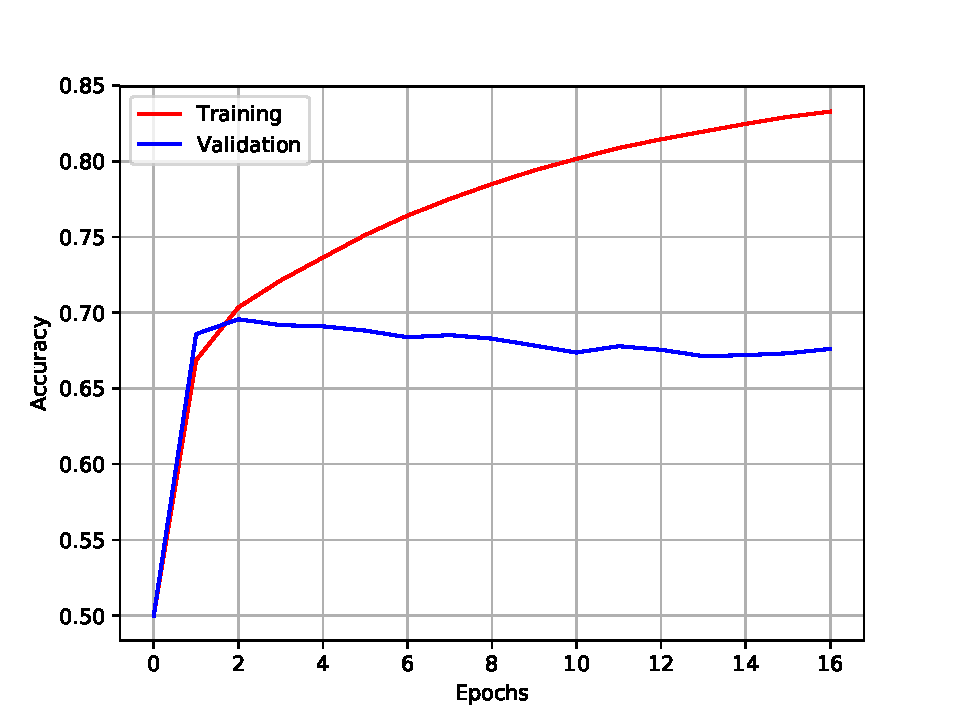
\includegraphics[width=0.5\textwidth]{./pictures/experiments/conv_char_word_nn/training}
    \caption{Training and validation accuracies of \gls{conv-char-word-NN}
        during training. We stop training when the validation accuracy no longer
        follow the training accuracy.}
    \label{fig:conv-char-word-NN-training}
\end{figure}

\begin{description}

    \item[Embedding:]

    Like in \gls{conv-char-NN} the embedding layers takes in a text as a
    stream of characters, where they are then mapped to a 5 dimensional vector
    space. There is not a very big difference here. In addition to that however,
    we also added the word channel used in \gls{rec-sent-NN}. This works in
    exactly the same way. It uses the pre-trained embeddings mentioned to map
    each word of the text in addition to mapping the characters. This is the
    basic idea of this network, a multi-channeled convolutional approach. Thus
    the network doesn't only take 2 inputs, in the form of two texts. It takes 4
    inputs, a character input for each each and a word input for each text. Both
    of these channels have their own path through the network. Which for ease of
    understanding can be seen as two different siamese networks.

    \item[Feature Extraction:]

    The feature extraction done in this network differs between the character
    network and the word network. Like previously, we make use of two different
    convolutional layers in the character network. They have a sliding windows
    size of 8 and 4, and a filter size of 200. This combination of window sizes
    had proven to work quite in the \gls{conv-char-NN}. It was because of this
    we saw no reason to actually change it, as the creation of this network was
    done in an additive manner. The addition can of course be found in the word
    network. The embedded stream of words are given to its own convolutional
    layer with a sliding window size of 8, and a filter size of 100.

    \item[Combining:]

    Due to the addition of the extra word network, the combining of step is
    has an additional step. The network initially combine the output of both
    the word and the character sub-networks. This is done by concatenating
    the output of the two convolutional layers in the character network, and
    the single convolutional layer in the word network. This results in two
    concatenated sets, one for each of the two texts. The elementwise absolute
    difference of the two sets are then computed, and passed along to the
    decision part of the network.

    \item[Decision:]

    The decision part of this network is simply 2, 500 unit fully connected
    layers followed by a 0.3 dropout layer. The output of that dropout layer
    is then given the 2 unit soft-max layer, for the final decision.

\end{description}

We have the network structure in Figure \ref{fig:conv-char-NN-model}.

\begin{figure}
    \centering
    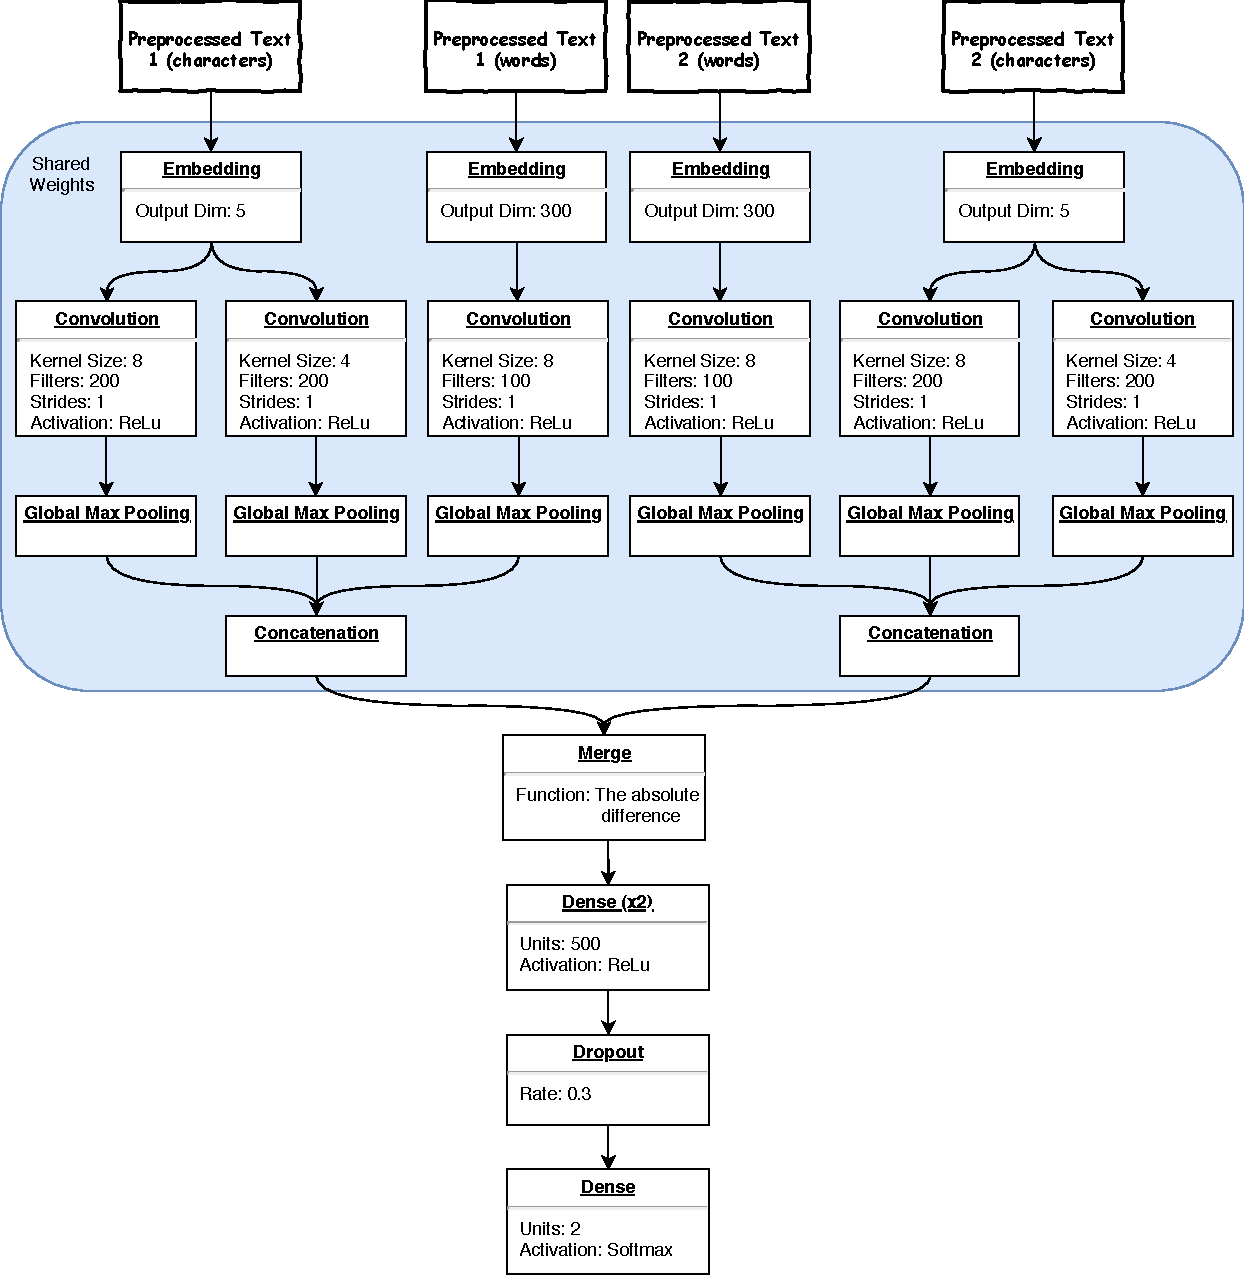
\includegraphics[width=\textwidth]{./pictures/experiments/conv_char_word_nn/model}
    \caption{The structure of network \gls{conv-char-word-NN}. The weights are
        shared from from the embedding layer all the way down to right before
        the four paths merge. The texts are given as both a sequence of
        characters and as a sequence of words. That allows the network to look
        at both. Different convolutions are trained for characters and words.}
    \label{fig:conv-char-NN-model}
\end{figure}

The path gone through to reach this design was a rather short one, compared
to to the two described above. The design of this network was derived based
on a combination of the other two network, the \gls{conv-char-NN}, and
\gls{rec-sent-NN}. The convolutional approach used on \gls{conv-char-NN},
showed promise, and this network was an attempt to improve on that.

Initially these alternations were small. They took the form on a different
amount of convolutional layers, with a differing amount of sliding window sizes.
These small changes also included the addition of regularization measures,
such as dropout layers. The largest change came when we incorporated the
multi-channel approach used in \gls{rec-sent-NN}. The thought process was,
that if character were good features for this task, another channel would
only provide additively better results. This was what yielded the network
described above, which works on the character level and the word level. 3
channel convolutional network were also produced during experimentation. Results
from that seemed to indicate that the linguistic level of sentences were too
high, thus hurting the model.

Similarly to the two other networks found the best prediction system and
tuned the threshold for this network. We try the same prediction systems
and thresholds as for the other two networks. We have shown the accuracy
and accusation error for the dataset containing 50\% negatives in Figure
\ref{fig:conv-char-word-NN-pred-50} and for the dataset containing 4\% negatives
in Figure \ref{fig:conv-char-word-NN-pred-4}.

\begin{figure}
    \centering
    \textbf{Prediction System Results for 0.5 Split, \gls{conv-char-word-NN}}\par\medskip
    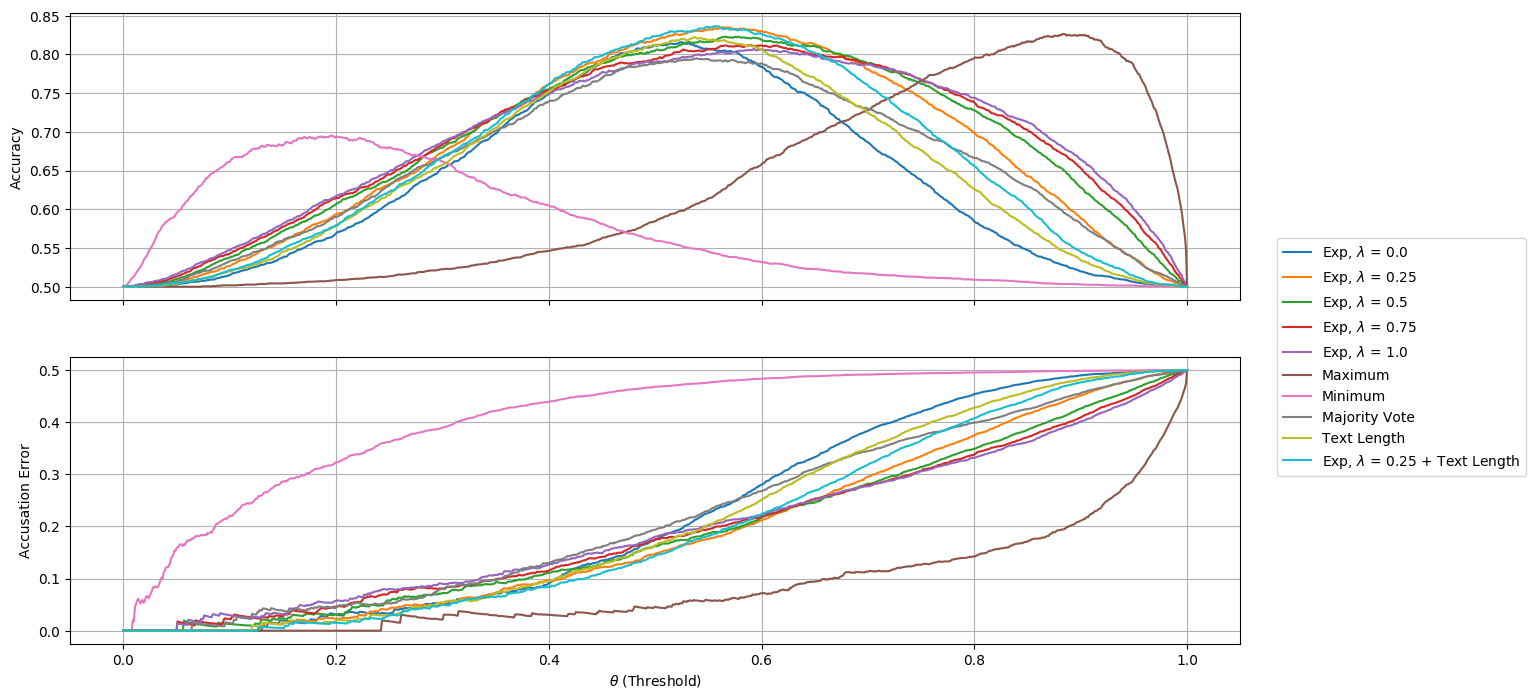
\includegraphics[scale=0.33]{./pictures/experiments/conv_char_word_nn/prediction_system_50}
    \caption{Results of running the prediction system with
        \gls{conv-char-word-NN} on a validation dataset with 50\% positive
        samples and 50\% negative samples. In the upper graph we show the
        accuracies obtained as a function of $\theta$ for different prediction
        systems. At the bottom we have shown the accusation error as a function
        $\theta$ again with one line for each prediction system. We can see that
        as the threshold increases and we accuse more people of cheating the
        accusation error rises.}
    \label{fig:conv-char-word-NN-pred-50}
\end{figure}

\begin{figure}
    \centering
    \textbf{Prediction System Results for 0.04 Split, \gls{conv-char-word-NN}}\par\medskip
    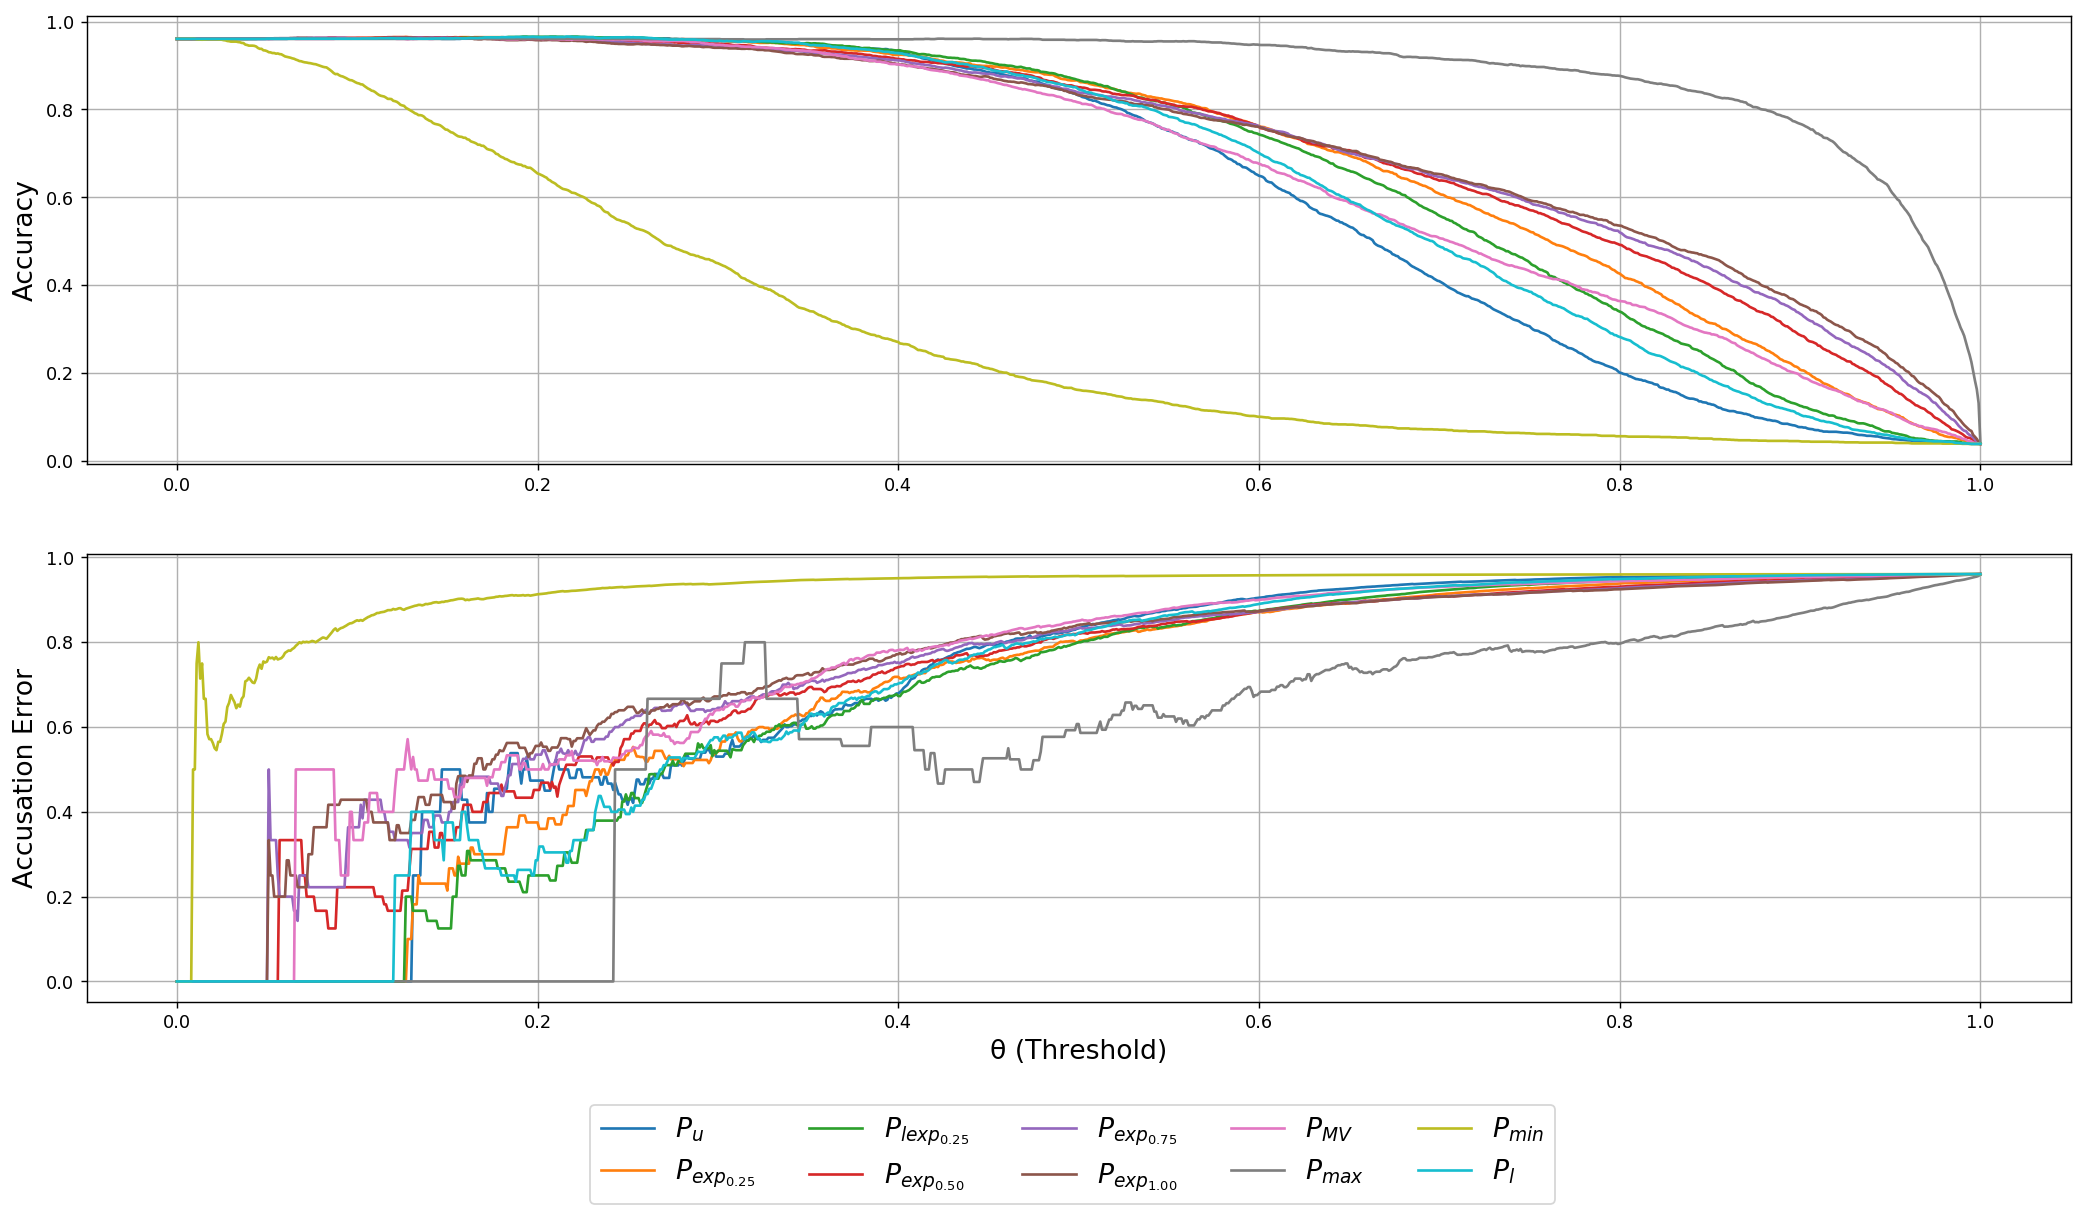
\includegraphics[scale=0.33]{./pictures/experiments/conv_char_word_nn/prediction_system_04}
    \caption{Results of running the prediction system with
        \gls{conv-char-word-NN} on a validation dataset with 96\% positive
        samples and 4\% negative samples. In the upper graph we show the
        accuracies obtained as a function of $\theta$ for different prediction
        systems. At the bottom we have shown the accusation error as a function
        $\theta$ again with one line for each prediction system. We can see that
        as the threshold increases and we accuse more people of cheating the
        accusation error rises.}
    \label{fig:conv-char-word-NN-pred-4}
\end{figure}

The best configuration for the 50/50 split and the 96/04 split was the
following,

\begin{center}
    \begin{tabular}{|c|c|c|c|c|c|c|c|c|}
        \hline
        Split & Weight            & $\theta$ & TP   & TN   & FP  & FN  & Acc     & A-Error \\ \hline
        50/50 & $P_{lexp_{0.25}}$ & 0.433    & 1856 & 1302 & 697 & 143 & 0.7898 & 0.099   \\ \hline
        96/04 & $P_{exp_{0.25}}$  & 0.127    & 1999 & 9    & 73  & 0   & 0.9649 & 0.000   \\ \hline
    \end{tabular}
\end{center}


\subsection{Summary}

In this section we described the experiments we performed. We started by
explaining how we selected the features our baselines work on. After that we
described how we performed the parameter selection for the baseline methods. We
then presented three different network architectures. Two convolutional and one
recurrent. The networks worked on different linguistic layers,

\begin{description}
    \item[\gls{conv-char-NN}] The character level,
    \item[\gls{rec-sent-NN}] The sentence level,
    \item[\gls{conv-char-word-NN}] Word and character level.
\end{description}

For each of the networks we used a validation set to determine the best
configurations for the prediction system. A summarizing view of the
validation performance of the different networks can be seen in Table
\ref{tab:experi-results}.

% TODO: This should probably not be called weights. The weights are now known as
% "prediction systems".
\begin{table}[h]
\begin{tabular}{|c|c|c|c|c|c|c|c|c|c|}
\hline
Split                  & Network                 & Weight            & $\theta$ & TP  & TN  & FP  & FN & Acc     & A-Error \\ \hline
\multirow{3}{*}{50/50} & \gls{conv-char-NN}      & $P_{lexp_{0.25}}$ & 0.390    & 1843 & 1482 & 517  & 156 & 0.8316 & 0.095   \\ \cline{2-10} 
                       & \gls{rec-sent-NN}       & $P_{lexp_{0.25}}$ & 0.033    & 1965 & 310  & 1689 & 34  & 0.5690 & 0.099   \\ \cline{2-10} 
                       & \gls{conv-char-word-NN} & $P_{lexp_{0.25}}$ & 0.433    & 1856 & 1302 & 697  & 143 & 0.7898 & 0.099   \\ \hline
\multirow{3}{*}{96/04} & \gls{conv-char-NN}      & $P_{mv}$          & 0.057    & 1999 & 8    & 74   & 0   & 0.9644 & 0.000   \\ \cline{2-10} 
                       & \gls{rec-sent-NN}       & $P_{lexp_{0.25}}$ & 0.002    & 1999 & 1    & 79   & 0   & 0.9620 & 0.000   \\ \cline{2-10} 
                       & \gls{conv-char-word-NN} & $P_{exp_{0.25}}$  & 0.127    & 1999 & 9    & 73   & 0   & 0.9649 & 0.000   \\ \hline
\end{tabular}
\caption{The performance of all neural networks we have implemented on the
    validation dataset.}
\label{tab:experi-results}
\end{table}

    \FloatBarrier

    \section{Results} \label{sec:results}

We have finally reached the point where we can determine the unbiased accuracy
of our different models. To do this we will make use of the \gls{D} dataset. As
mentioned in Section \ref{sec:data}, this dataset consists of 3558 authors, none
of which are repeated in any of the other sets.

We have 5 models which we are going to apply to this test dataset, our
two baseline methods, the \gls{conv-char-NN}, the \gls{rec-sent-NN} , and the
\gls{conv-char-word-NN}.

Starting with the baseline methods, we made use of the features and the
hyper parameters that provided best on the training set. For the extended
delta method, the optimal parameters were $K=1$ and $p = 1$. Then using
the same sample generation as was described in the bottom of Section
\ref{sec:hyp_select}, and normalizing using the scaler produced when generating
the features, we applied were able to apply the model. The same was done with
the \gls{SVM}, where we used the optimal found hyperparameters, $C=10$ and
$\gamma = 1000$, to train the model.

As briefly mentioned in Section \ref{subsec:baseline_methods}, these methods are
not very well suited for this particular task. Since they both provide binary
results denoting a students' innocence, or lack thereof, it is not possible to
apply any kind of thresholding to force our models under the 10\% accusation
error goal. They always perform at their maximum capacity. For this reason we
had to alter the way we compare the deep learning approaches with our baselines.
This was done by determining the best performing threshold ($\theta$) and weight
function for our neural network with regard to accuracy, and with no regard to
the accusation error, as both our baselines do not focus on that either. Thus we
compared the results of our baselines on the 50/50 dataset and the 96/04 dataset
with the highest unconstrained accuracy our \gls{NN} methods could muster.

After determining the best networks using the dataset \gls{E} in conjunction
with dataset \gls{F}, we proceeded to train the three networks on the entire
dataset \gls{B} using dataset \gls{C} as the validation set used throughout the
training. Doing this, was all for the sake of providing more data for the final
models, before applying them to the \gls{D} test dataset.

Having now trained the models we can determine the accuracy and accusation error
of our different networks, both with and without the 10\% accusation error
constraint. It should be noted that the parameters found that adhere to to the
10\% constraint were found on the training data. As with any machine learning
approach, this does not ensure the same level of adherence on the test data.

We also used that same approach for the other two networks. The combined
results for the 50/50 split test dataset \gls{D} can be seen in Table
\ref{tab:50_results}, and the results for the 96/04 split data can be seen in
table \ref{tab:04_results}.

\begin{table}[]
\centering
\textbf{The results of running our methods on a 50/50 split test dataset}\par\medskip
\begin{tabular}{|c|l|c|c|c|c|c|c|c|c|}
\hline
Bound                & Method                  & Weight            & $\theta$ & TP  & TN  & FP  & FN  & Acc             & A-Error         \\ \hline
\multirow{5}{*}{Yes} & SVM                     & \multicolumn{8}{c|}{N/A}                                                                     \\ \cline{2-10} 
                     & Extended Delta          & \multicolumn{8}{c|}{N/A}                                                                     \\ \cline{2-10} 
                     & \gls{conv-char-NN}      & $P_{lexp_{0.25}}$ & 0.390    & 3392 & 2344 & 1206 & 158  & \textbf{0.8078} & \textbf{0.0631} \\ \cline{2-10} 
                     & \gls{conv-char-word-NN} & $P_{lexp_{0.25}}$ & 0.433    & 3185 & 2512 & 1038 & 36   & 0.8023          & 0.1268          \\ \cline{2-10} 
                     & \gls{rec-sent-NN}       & $P_{lexp_{0.25}}$ & 0.033    & 3182 & 1470 & 2080 & 368  & 0.6552          & 0.2002          \\ \hline\hline
\multirow{5}{*}{No}  & SVM                     & N/A               & N/A      & 2667 & 2442 & 1100 & 883  & 0.7195          & 0.2656          \\ \cline{2-10} 
                     & Extended Delta          & N/A               & N/A      & 2349 & 2064 & 1486 & 1201 & 0.6215          & 0.3678          \\ \cline{2-10} 
                     & \gls{conv-char-NN}      & $P_{lexp_{0.25}}$ & 0.486    & 3231 & 2913 & 637  & 319  & \textbf{0.8653} & \textbf{0.0987} \\ \cline{2-10} 
                     & \gls{conv-char-word-NN} & $P_{lexp_{0.25}}$ & 0.544    & 2810 & 3088 & 462  & 740  & 0.8307          & 0.1933          \\ \cline{2-10} 
                     & \gls{rec-sent-NN}       & $P_{lexp_{0.25}}$ & 0.267    & 1795 & 3076 & 474  & 1755 & 0.6860          & 0.3632          \\ \hline
\end{tabular}
\caption{The results on the 50/50 dataset, using the listed methods.
\textit{Bound} refers to wether or not $\theta$ and the Weight which we used,
was chosen based on their accuracy bounded/constrained by a 0.1 accusation error.
In the case of Yes, it refers to under the 0.1 threshold and No refers to simply
maximizing accuracy with no regard for accusation error. In both case
the best results were bolded.}
\label{tab:50_results}
\end{table}

\begin{table}[]
\centering
\textbf{The results of running our methods on a 96/04 split test dataset}\par\medskip
\begin{tabular}{|c|l|c|c|c|c|c|c|c|c|}
\hline
Bound                & Method                  & Weight            & $\theta$ & TP  & TN & FP & FN  & Acc             & A-Error         \\ \hline
\multirow{5}{*}{Yes} & SVM                     & \multicolumn{8}{c|}{N/A}                                                                   \\ \cline{2-10} 
                     & Extended Delta          & \multicolumn{8}{c|}{N/A}                                                                   \\ \cline{2-10} 
                     & \gls{conv-char-NN}      & $P_{MV}$          & 0.057    & 3546 & 13  & 140 & 4    & \textbf{0.9611} & \textbf{0.2352} \\ \cline{2-10} 
                     & \gls{conv-char-word-NN} & $P_{exp_{0.25}}$  & 0.127    & 3516 & 32  & 112 & 34   & 0.9604          & 0.5151          \\ \cline{2-10} 
                     & \gls{rec-sent-NN}       & $P_{lexp_{0.25}}$ & 0.002    & 3505 & 18  & 130 & 45   & 0.9526          & 0.7142          \\ \hline\hline
\multirow{5}{*}{No}  & SVM                     & N/A               & N/A      & 2629 & 98  & 57  & 921  & 0.7372          & 0.9038          \\ \cline{2-10} 
                     & Extended Delta          & N/A               & N/A      & 2369 & 92  & 56  & 1181 & 0.66549         & 0.9277          \\ \cline{2-10} 
                     & \gls{conv-char-NN}      & $P_{lexp_{0.25}}$ & 0.137    & 3540 & 28  & 125 & 10   & \textbf{0.9635} & \textbf{0.2631} \\ \cline{2-10} 
                     & \gls{conv-char-word-NN} & $P_{lexp_{0.25}}$ & 0.192    & 3507 & 47  & 97  & 43   & 0.9621          & 0.4777          \\ \cline{2-10} 
                     & \gls{rec-sent-NN}       & $P_{lexp_{0.25}}$ & 0.002    & 3505 & 18  & 130 & 45   & 0.9526          & 0.7142          \\ \hline
\end{tabular}
\caption{The results on the 96/04 data set, using the listed methods.
\textit{Bound} refers to wether or not $\theta$ and the Weight which we used,
was chosen based on their accuracy bounded/constrained by a 0.1 accusation error.
In the case of Yes, it refers to under the 0.1 threshold and No refers to simply
maximizing accuracy with no regard for accusation error. In both case
the best results were bolded.}
\label{tab:04_results}
\end{table}

    \FloatBarrier

    \section{Discussion} \label{sec:discussion}

In this section we discuss the results of our experiments, our expectations
compared to the actual performance. In addition to that we also address the
real world applicability of our produced methods. This includes areas such as
scalability, teacher feed/assistance and model implementation.


\subsection{Results}

We presented the results of our experiments on the test dataset in Section
\ref{sec:results}. Here we discuss those results. We will focus on the results
on a dataset with 4\% negatives as that reflects the real world. For the
networks we use the constrained results while for the baselines we use the
unconstrained results. We reported three properties for each method, accuracy,
accusation error and specificity. None of our methods achieved an accusation
error of below 10\% as MaCom required. The closest method to achieve such
a low accusation error was the \gls{conv-char-NN} network. The baselines
both had higher accusation error than any of the networks on more than 90\%.
The highest specificity was achieved by the baseline methods and of the
networks the \gls{conv-char-word-NN} achieved the highest specificity. As the
accusation error was the most important measure for MaCom we conclude that the
\gls{conv-char-NN} was the best network even though it did not have the highest
specificity.

We believe that some of the methods show promising results. The
\gls{conv-char-NN} had the highest overall accuracy in all the categories we
tested it on. It was closely followed by network \gls{conv-char-word-NN}. The
\gls{rec-sent-NN} had sub-par performance. It is however worth noting that this
could very well be due to the infeasibility of running any of our \glspl{RNN} on
the character or word level. We hypothesize that the accuracy of an \gls{RNN}
would be greatly increased had it been run on a lower linguistic level. In
experiments we found that \glspl{CNN} also performed badly on the sentence level
in our use case. Unfortunately we were not able to train an \gls{RNN} on one of
the lower linguistic levels due to computational constraints.

When comparing our validation dataset results from Table
\ref{tab:experiment-validation-results} to our test results we can clearly see a
difference. The results from the validation dataset meets the requirements for
the accusation error, while the test results does not. However, this difference
is justified as it was on the validation set that we found the prediction system
and threshold that got us under said requirement. Therefore it stands to reason
that the models would have a somewhat lower performance when applied to a fresh,
untouched test dataset. This lowered performance takes form of an increased
accusation error, and a decreased accuracy.

It is worth noting that the number of false accusations on the validation
dataset were very small. It seems like we have overfitted a lot on the
validation dataset and found the exact point before many false accusations were
made. We should have maybe used a slightly lower threshold such that we would
not have achieved such a high accusation error on the test dataset.


\subsubsection{AUROC}

A more general metric of a model's performance can be computed using the
\gls{AUC} of the \gls{ROC}-curve of a model better known as \gls{AUROC}.
A \gls{ROC} curve is the \gls{FPR} plotted against the \gls{TPR} both of
which are defined in Section \ref{sec:method}. \gls{AUROC} is a measure of
discrimination, or a measure of the amount of certainty our model has when it
makes a decision.

The ROC curves and AUROC results for the different networks we produced
can be seen in Figure \ref{fig:AUROC}. These figures reinforce the
previously stated relationship between the different networks. The
\gls{conv-char-NN} still performed best. It was however very closely followed
by the \gls{conv-char-word-NN}. At some points the two \gls{ROC}-curves overlap
when using the dataset with 4\% negative samples and with the constrained
configuration.

While the \gls{rec-sent-NN} does have the worst AUROC score it is higher
than we anticipated when looking back at the results presented in Section
\ref{sec:results}. 

\begin{figure}
    \centering
    \begin{minipage}{.8\textwidth}
        \centering
        \textbf{Constrained ROC-Curve and AUROC for each network}
        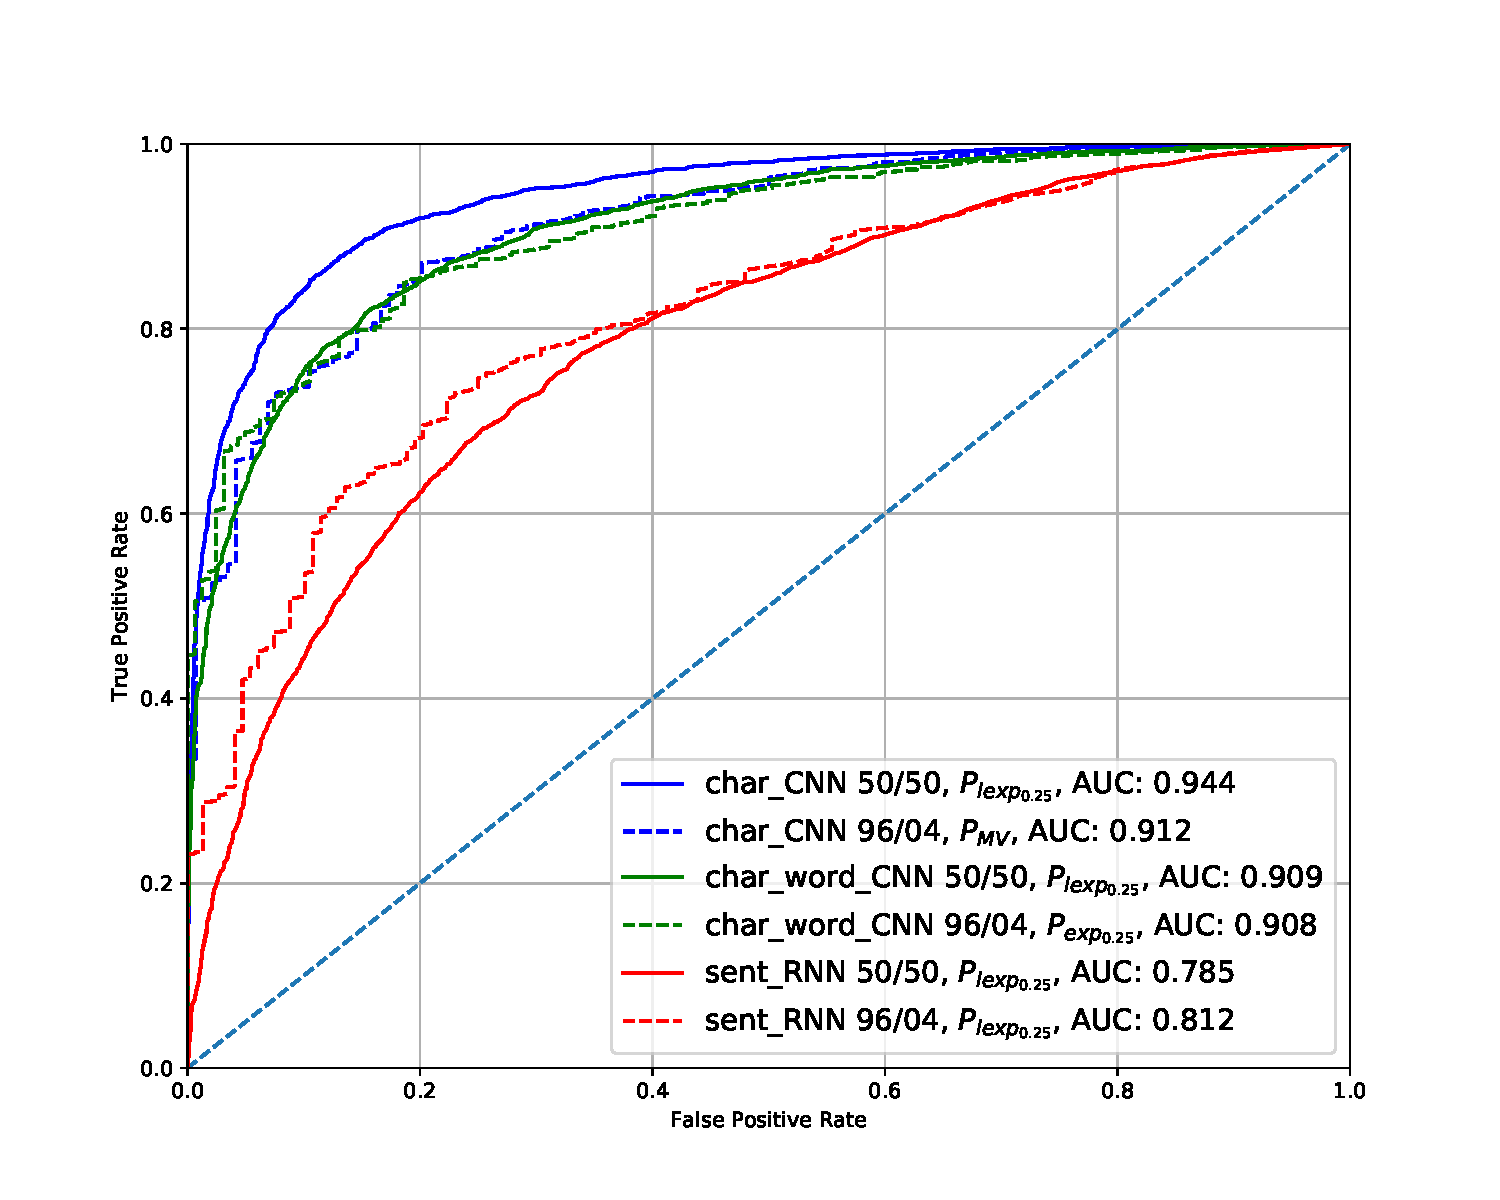
\includegraphics[width=1\linewidth]{./pictures/discussion/AUROC_Constrained}
    \end{minipage}\\
    \begin{minipage}{.8\textwidth}
        \centering
        \textbf{Unconstrained ROC-Curve and AUROC for each network}
        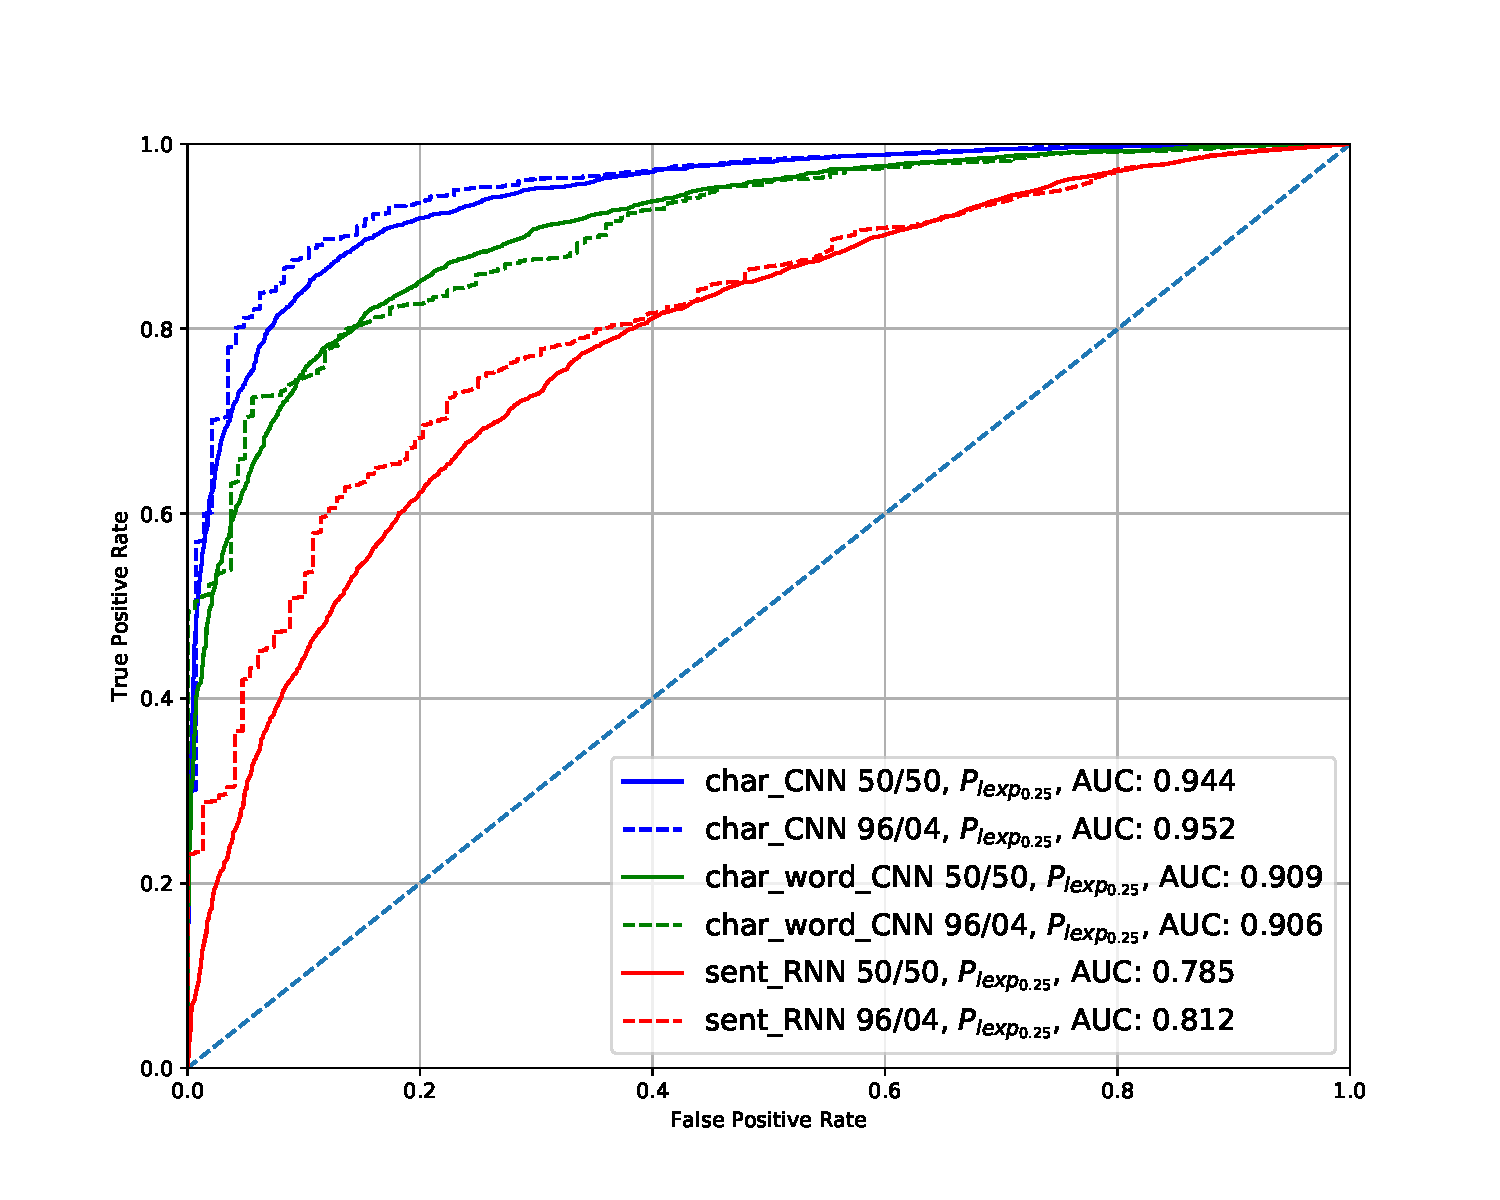
\includegraphics[width=1\linewidth]{./pictures/discussion/AUROC_Unconstrained}
    \end{minipage}
    \caption{The \gls{ROC}-curve for the three networks produced plotted for
        both of the possible data sample splits. We used the configuration of
        threshold and prediction system that produced the best results on the
        validation dataset \gls{C}.}
    \label{fig:AUROC}
\end{figure}

Our \gls{AUROC} scores are generally very good. We can see in the figures that
the score on the 50\% negative dataset is about the same as on the
4\% negative dataset. Our reported results (not \gls{AUROC} score) looks much
worse on the 4\% dataset but it is also much harder to achieve a good results on
a dataset with such few negatives. The \gls{AUROC} scores show that we retain a
good discriminative model even when the dataset changes to match the real world
data.


\subsubsection{Comparison Between Methods}

When comparing our two convolutional networks we see that the \gls{conv-char-NN}
has the highest accuracy and lowest accusation error. Recalling that the
\gls{conv-char-NN} works on the character level and the \gls{conv-char-word-NN}
works on both the character and word level it would seem as if the word level
does not contribute much to the classification. However we have to keep in
mind that the \gls{conv-char-NN} generally had more resources available. We
used more time experimenting on that network and it had more dense layers and
more convolutions available. We would have liked to have experimented more
with different linguistic layers. It would have been especially interesting
to develop a network using both the character, word, sentence and \gls{POS}
tag level. It would also have been interesting to create a version of the
\gls{conv-char-word-NN} that had as many character level convolutions as the
\gls{conv-char-NN} and as many dense layers but then had a separate word level
input channel. Then we would have been able to conclusively determine whether or
not a word channel was worth it in our network architecture.

Comparing our convolutional networks and our recurrent network we see that
the convolutional networks performs much better. We briefly discussed in
Section \ref{subsubsec:siamese_networks} the advantages and disadvantages of
\glspl{CNN} vs \glspl{RNN}. The discussion was based on a comparative study by
\citep{DBLP:journals/corr/0001KYS17}. The conclusions of the study was that both
recurrent and convolutional networks works well for \gls{NLP} but that they
work well for different problem types. If the content of a text is important
for solving a specific problem such as for \textit{Automatic Text Summation}
\glspl{RNN} works best \citep{DBLP:journals/corr/ZengLFU16}. Similarly if the
content is not important such as authorship verification tasks convolutional
networks generally works better \citep{DBLP:journals/corr/0001KYS17}. Our
results back up that finding. We found that it was much easier to develop a
convolutional neural network that worked well in our setting than a recurrent
neural network.


\subsubsection{Previous Work on MaCom Data}

In Section \ref{subsec:previous_work_using_macoms_dataset} we describe other
experiments with authorship attribution and verification on MaCom's dataset.
In this section we compare our authorship verification results with those
earlier results. The first experiment we compare against is \citep{aalykke2016}.
\citet{aalykke2016} evaluated his performance using the sensitivity and
specificity of his best performing configuration. The sensitivity is reported at
95.0\% and the specificity at 71.9\%. Those results were obtained on a dataset
with 500 positive cases and 500 negative cases. \citet{aalykke2016} commented
that his results were not directly comparable to the real world as he used a
dataset with 50\% negative samples. We have focused on developing methods that
work best on a dataset with 4\% negative samples. We have however reported
results when maximizing accuracy on a 50\% negative dataset which is comparable
to his results. In our best configuration on the 50\% negative dataset, we
obtained a sensitivity of 91.0\% and a specificity of 82.1\%. That means that
we had a worse sensitivity but a better specificity. The accuracy obtained by
\citet{aalykke2016} was $\frac{0.95 + 0.719}{2} = 83.5\%$ while our accuracy was
at $86.5\%$, so we had a higher accuracy.

The results produced by \citet{aalykke2016} are impressive considering he only
used the distances between feature sets to compare assignments. One caveat to
consider when looking at his results compared to ours is the fact that he tried
all thresholds on the test dataset and reported the best results obtained.
The results we report used a configuration found on a validation dataset and
evaluated on a test dataset. We can therefore expect that our results will be
an unbiased estimate of real world performance while the best results produced
by \citet{aalykke2016} will probably not. Furthermore \citet{aalykke2016} used
a test dataset that only contained \gls{SRP} assignments. In our test dataset
we predict the newest text in an author's library which is not necessarily the
\gls{SRP} assignment. That gives \citet{aalykke2016} another advantage since
the \gls{SRP} assignments are generally longer assignments and therefore give a
better picture of an author's writing style.

To summarize, \citet{aalykke2016} have a lower accusation error than we do
with 5\% (100\% - 95\%) vs our 9.87\%. At the same time they also have a lower
specificity of 71.9\% vs our 82.1\%. So which method to use is a tradeoff
between how many false accusations to allow vs how large a fraction of cheaters
they want to catch. We believe that our method would have obtained better results if
we had used a test dataset of only \gls{SRP} assignments. For future work,
such a test could be relevant as well as interesting.

We also compare our results with another experiment. This experiment was
described in \citep{hansen2014}. They measured their results using a simple
accuracy. They achieved a maximum accuracy of 84\%. They did not specify the
fraction between negatives and positives that they evaluate against. We assume
that they evaluate on a 50/50 percent split as \citet{aalykke2016}. Again our
most comparable result is when we maximize accuracy on a 50/50 split. Our
best accuracy in that setting were 86.54\%. \citet{hansen2014} focused on the
computation time of their method. Since they used an author specific model they
had to train a separate model on each new author and a new model each time an
author turned in a new assignment. That is where our generalizing model has an
advantage. We only have to train the model once and after that it can be used
on any new author. The prediction time of a neural network is lower than the
training time of an \gls{SVM}.

\citet{hansen2014} found that recent texts were more important than older
texts for predicting an author's writing style. During our experimentation
we came to that same conclusion. The better configurations we found
used a prediction system based on the time in which the assignments were
turned in. We will discuss how students writing styles evolve in Section
\ref{subsec:writing_style_changes}.

We seem to have a very comparable but slightly better performance than previous
experiments that made use of MaCom's dataset. Our results are not significantly
better, but we have several advantages over previous methods. We have focused
on performance on a dataset split with 96\% positives and 4\% negatives, and we
have implemented a generalizing model. The data split means that our results are
more reliable as estimates of real world performance, and the generalizing model
means that we save computation time.


\subsubsection{Other Authorship Verification Results}
\label{subsubsec:other_authorship_verification_results}

As described earlier \citet{qian:2018} received excellent authorship
verification results. They achieved an accuracy of 99.8\%. We based our
recurrent network on their architecture as we wanted to replicate their results.
Our recurrent network had nowhere near as high accuracy as we achieved an
accuracy of 68.6\% on the test dataset. We had not suspected our results to be
exactly as good as \citet{qian:2018}, but a drop that big was not expected.
However, there are some important differences between the datasets the networks
are trained and tested on.

The dataset \citet{qian:2018} used were the Reuter\_50\_50 dataset
\\\citep{Dua:2017}. It contains 50 authors each with 100 texts. For each
author 50 of his/her 100 texts were in the training dataset and 50 were in
the testing dataset. Furthermore the texts were all from the same topic
(corporate/industrial). In contrast, our dataset uses completely different
authors between the training and test dataset and we have texts spanning many
topics.

At one point we trained a network using the \citet{qian:2018} inspired
architecture on a training and validation dataset using the same authors. Here
we observed that the validation accuracy followed the training accuracy far
longer than was the case for a validation dataset containing different authors.
We therefore believe that the reason \citet{qian:2018} obtained such good
results is that the test and training datasets consisted of the same authors. We
wanted to create a generalizing model that were trained once and used many times
which meant that this architecture did not work as well for our purpose.

An interesting area for further research and experimentation could be creating
a combination between our generalizing models and author specific neural
network models. A disadvantage when using author specific models is that it
is necessary to train a different model for each author and retrain models
when new material is turned in by an existing author. However they have the
advantage of often being more accurate than generalizing models. We could have
used our generalizing model to find potential ghostwriting candidates. Using
the \gls{conv-char-word-NN} we could catch 32.6\% of the ghostwriters on a 4\%
negative dataset but we could only do so with an accusation error of 47.7\%. We
could stop taking the output of the generalizing model as the truth, and then
use a author specific network to verify the result of the generalizing model.
Then we would only be required to train a generalized model in the cases where
we suspect ghostwritten assignments.


\subsection{Teacher Feedback}\label{subsec:teacher_feedback_text_comparisons}

As mentioned in Section \ref{sec:introduction} we wanted to explore what kind
of feedback we could give teachers in conjunction with the bare predictions.
As explained earlier the system is not meant to be the final judge of which
students are cheating but is rather meant as a support system for teachers that
are already suspicious of a student. We have focused on the \gls{conv-char-NN}
network since it performed best on the test dataset.


\subsubsection{Extracting Important Features}

Previously we have looked at the output of the feature extraction layer to
obtain information on what a specific network was looking at during the
creation of the networks. We wanted to do something similar for teacher
feedback. Recall that the \gls{conv-char-NN} started with a convolutional
layer followed by a max pool layer. For that reason the larger output of a
convolution is considered the most important one for a particular sequence.
An example of how this feature extraction process works, can be seen in
\ref{fig:feature_extraction_output_example}. Each filter gives a single output
that is the maximum output of any filter position. The combining function for
the \gls{conv-char-NN} is the absolute difference. This means that when we
compare texts $t$ and $t'$, the output of the combination will be high for
a particular filter iff the maximum output of that filter is significantly
different for $t$ and $t'$.

\begin{figure}
    \centering
    \textbf{Teacher Feedback Example}\par\medskip
    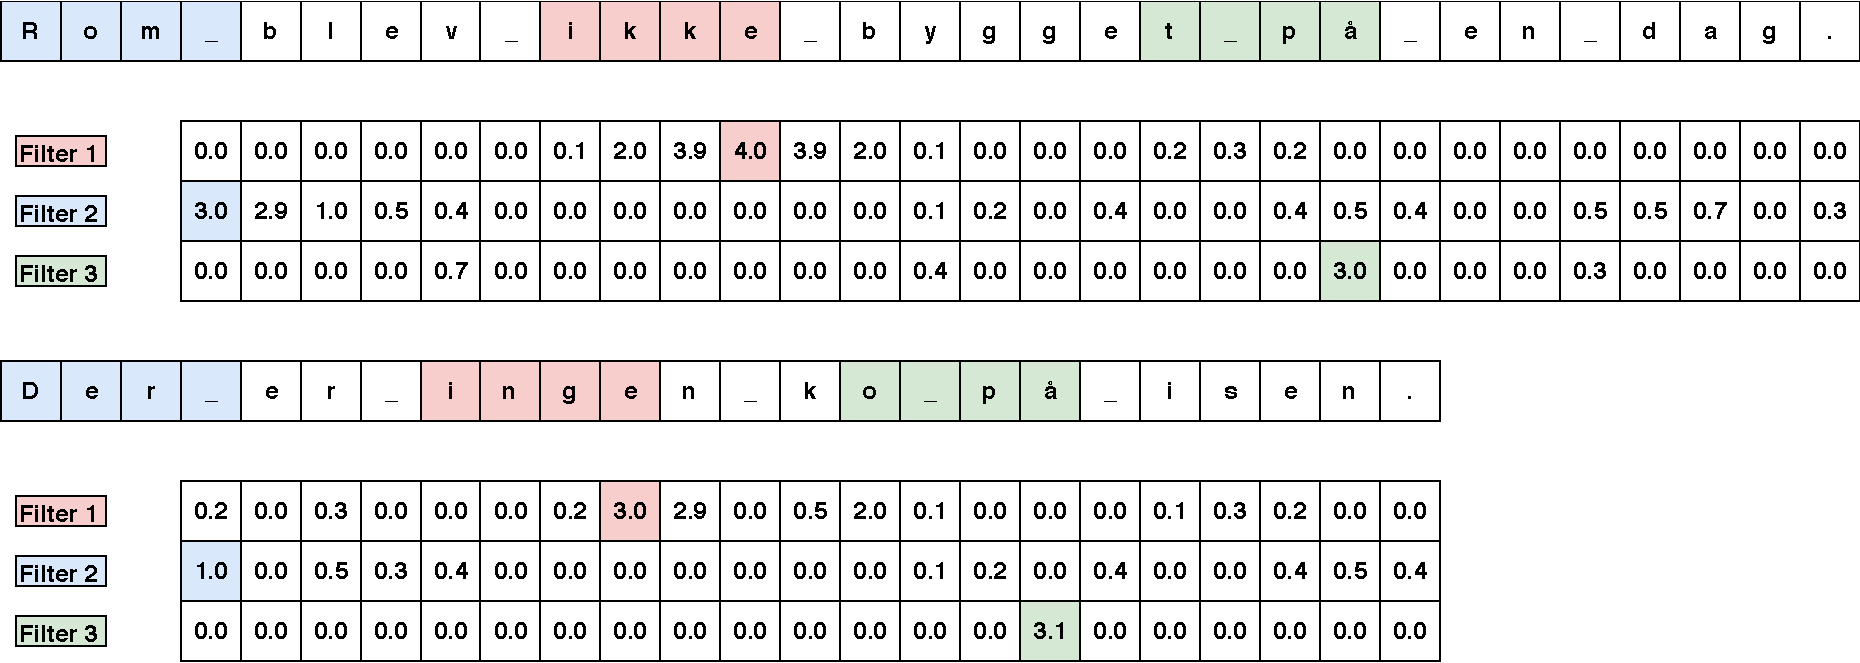
\includegraphics[width=\textwidth]{./pictures/discussion/teacher_feedback_example}
    \caption{Illustrates our feedback to teachers. The particular network
    used in this example only has three filters. The three filters' maximum
    activations are shown in three different colors for the two texts they are
    comparing. The first filter looks for negative qualifiers. Therefore, it
    reacts strongly to both the Danish word "ikke" (not) and part of the Danish
    word "ingen" (none). The second filter looks for city names and reacts
    strongly to the string "Rom " (Rome) but less strongly to "Der " (not a city
    name) even though it looks like a city name. The third filter reacts to
    phrases that contains the word "p\aa " (on) and therefore reacts equally to
    both texts}
    \label{fig:feature_extraction_output_example}
\end{figure}

It is hard to know exactly what the following layers do with the absolute
difference, but we hypothesize that the largest filter differences translate to
the most important differences. The feedback system we implemented for teachers
takes an author $\alpha$, text $t$ and $n \in \mathbb{N}^+$ and outputs the $n$
largest differences between each $t' \in T_\alpha$ and $t$. The idea is that
when our system reports a negative, the teacher can ask for feedback from the
system. The teacher will then receive a list of the $n$ greatest differences
between each of the texts and can use that information to strengthen the claim
that a student used a ghostwriter.

As an example, we ran our system on a random author and a text 
that author did not write. The whole output can be seen in Appendix
\ref{subsec:teacher_feedback_text_comparisons}. We have shown a truncated
output in Table \ref{tab:teacher_feedback_output}. The output contains only
the comparison between one of the candidate authors' texts and the unknown
text. Text 1 is from the candidate author and Text 2 is the unknown text. 
The three substrings that generated the highest values on dataset \gls{C}
are used to illustrate what each of the filters are looking at.

\begin{table}
    \begin{tabular}{lll|lll}
        \textbf{Max 1}    & \textbf{Max 2}    & \textbf{Max 3}       &
        \textbf{Text 1}   & \textbf{Text 2}   & \textbf{Difference}  \\
        \hline
        \verb[nemlig 1[   & \verb[nemlig 1[   & \verb[nemlig –[      &
        \verb'pere.\n\nH' & \verb'nemlig b'   & |3.06 - 4.70| = 1.64 \\

        \verb[, F.eks.[   & \verb[, F.eks.[   & \verb[, F.eks.[      &
        \verb'. F.eks.'   & \verb'del. Und'   & |4.73 - 3.18| = 1.55 \\

        \verb[ke …''. [   & \verb[a...''\n\n[ & \verb[n''. '' [      &
        \verb'v. Men d'   & \verb'n. Den v'   & |4.28 - 2.91| = 1.37 \\

        \verb[forsøger[   & \verb[forsøger[   & \verb[forsøger[      &
        \verb'for sætt'   & \verb'forsøgte'   & |3.40 - 4.77| = 1.37 \\

        \verb[, Hvorda[   & \verb[, Hvorda[   & \verb[,08 – 6,[      &
        \verb', som ti'   & \verb', Hvorda'   & |3.70 - 5.07| = 1.37 \\

        \verb[der; ’’M[   & \verb[der; ”Ha[   & \verb[der; ”Ma[      &
        \verb'dem; Nia'   & \verb'der omha'   & |4.64 - 3.28| = 1.36 \\

        \verb[. Her ef[   & \verb[. Her ef[   & \verb[' Her br[      &
        \verb'. Jeg vi'   & \verb'. Her fo'   & |2.61 - 3.92| = 1.31 \\

        \verb[r dog kr[   & \verb[r dog kr[   & \verb[r dog ’d[      &
        \verb'r og lud'   & \verb'r dog i '   & |2.83 - 4.13| = 1.30 \\

        \verb[11], da [   & \verb[:1], da [   & \verb[:1], da [      &
        \verb'ys”, der'   & \verb'for, da '   & |3.78 - 5.04| = 1.26 \\

        \verb[, så Car[   & \verb[, så Car[   & \verb[, så Car[      &
        \verb', så er '   & \verb', som En'   & |5.19 - 3.94| = 1.25 \\
        \hline
        \verb[; ’S[       & \verb[; ’S[       & \verb[; ’E[          &
        \verb'; Ni'       & \verb'r He'       & |3.12 - 1.78| = 1.34 \\

        \verb[; ”t[       & \verb[; ”t[       & \verb[; ”t[          &
        \verb'; ”H'       & \verb', ”j'       & |3.44 - 2.13| = 1.31 \\

        \verb[d.’ [       & \verb[d.’ [       & \verb[d.’ [          &
        \verb'ne-V'       & \verb'20’e'       & |1.75 - 2.77| = 1.02 \\

        \verb[1\n’’[      & \verb[1]’’[       & \verb[1]’’[          &
        \verb' l2-'       & \verb'720’'       & |1.75 - 2.71| = 0.96 \\

        \verb['Det[       & \verb['Det[       & \verb['Det[          &
        \verb'ndet'       & \verb' Det'       & |2.37 - 3.25| = 0.88 \\

        \verb[f 1"[       & \verb[f 1"[       & \verb[f 1"[          &
        \verb'f 2\n'      & \verb'v og'       & |3.05 - 2.20| = 0.85 \\

        \verb[æk''[       & \verb[’’ é[       & \verb[ud;'[          &
        \verb'lv; '       & \verb',tro'       & |2.60 - 1.77| = 0.83 \\

        \verb[\n\nx\n[    & \verb[\n\nx\n[    & \verb[\n\nx\n[       &
        \verb'\n\n\n\n'   & \verb'\n\n5\n'    & |1.81 - 2.61| = 0.80 \\
        \verb[ “… [       & \verb[ “… [       & \verb[?“! [          &
        \verb'nd” '       & \verb'r,” '       & |1.75 - 2.53| = 0.78 \\

        \verb[S\n, [      & \verb[S\n, [      & \verb[O\n, [         &
        \verb'e\n, '      & \verb'ad, '       & |2.62 - 1.92| = 0.70 \\
    \end{tabular}

    \caption{Shows the 10 most different activations of convolutional filters
    on two different texts. Both the 10 most different activations for the
    filters of size 8 and size 4 are shown. What each filter is looking at is
    represented by the three greatest activations on any text in the \gls{C}
    dataset. The strings the filter reacted most to are shown in column
    \textbf{Text 1} and column \textbf{Text 2}. The actual activation values
    are shown in the column \textbf{Difference} where the left number corresponds
    to text 1 and the right to text 2. The filters are sorted so the
    greatest difference activation is at the top and the differences fall as we
    move down the list.}

    \label{tab:teacher_feedback_output}
\end{table}

Some of the filters are very clear about what they look at while others require
some parsing. One of the easier filters considers the filter activation
triggered by the string "F. eks". That phrase is Danish for "for example" or
"for instance" and some people write that as "for eksempel" while others use the
shorthand above. If this suddenly changes it could indicate that you are not the
author of an assignment. That cannot be the only reason given, but if thousands
of those reasons are present you can say with some confidence that someone else
has written the assignment. As an example of one of the harder to parse filters
consider the filter looking at \verb["ke …''."[, \verb["a...''\n\n"[ and
\verb["n''. '' "[. That filter seems to react to non-alphanumeric characters,
but on the two texts we are comparing none of the reactions look anything like
what gives the highest numbers. Instead the filter seems to also pick up on the
start of sentences.


\subsubsection{Locating Ghostwritten Areas}
\label{subsubsec:ghost_written_areas}

Aside from feedback based on an entire text, we looked at whether or not we
could say something about which parts of an assignment is most likely to be
ghostwritten. That would allow a suspicious teachers to identify the part of
the assignment which is least likely to be written by the student and further
analyze that small subsection of the assignment. To find the parts of a text
$t$ most likely to be ghostwritten we split $t$ into a list of paragraphs.
Each paragraph is separated by at least 2 newline characters. We throw away
paragraphs of less than 100 characters since it does not make sense to predict
on such a small amount of text. Hereafter we use one of our networks to compare
each individual paragraph against all of the author's other texts. We take the
average of the comparisons and can then report which paragraphs in the file are
least similar to the author's other texts.

To see how well that system worked we looped through each $\alpha \in
\mathcal{A}$ where $\mathcal{A}$ is the \gls{C} dataset. For each $\alpha$ we
chose a random text $t$ with more than 5 paragraphs. We then split that text up
into paragraphs and removed all paragraphs except the first 5. We then chose
a text $t' \not\in T_\alpha$ and chose a random paragraph from that text. We
then used \gls{conv-char-NN} to predict the 5 paragraphs from $t$ and single
paragraph from $t'$ against each $t'' \in T_\alpha \setminus \{t\}$. We computed
the average prediction on each of the 5 first paragraphs in $t$ and the average
prediction of the one paragraph from $t'$. We expect that the average prediction
on paragraphs from $t$ is higher than the paragraph from $t'$.

The predictions on the 5 paragraphs from $t$ was 0.42216, 0.43975, 0.44447,
0.44543 and 0.44425 while the prediction on the paragraph from $t'$ was 0.39524.
As expected we see that the paragraph from text $t'$ has a lower average score
than the 5 paragraphs from $t$. The difference is not as large as we would
have expected however. It seems as if the difference is small enough that
we cannot rely on the results when used on a single assignment. It is also
interesting that no predictions have above 50\% chance of being written by
$\alpha$. It seems like our network does not work well on texts as short as
a single paragraph. That makes sense since the network works by extracting
information from 1200 global max pools and comparing the output from two texts.
Short texts will not be able to achieve an activation of a enough of the filters
for it to be similar to a longer text. The character limit we chose in this
experiment was 100 characters while it was 400 when we trained the networks
which might also be part of the reason.

It is also interesting that the first two paragraphs from $t$ received a lower
average score than the last 3. It seems like the network is better at predicting
the middle of a text than the start of a text.

Another usage for the single paragraph predictions could be for classification
of group assignments. By using the prediction of each paragraph against the
collaborators behind the assignment. It could also be used to detect what amount
of a group assignment was written by what member of said group.


\subsubsection{Applying Other Machine Learning Methods}
\label{subsubsec:applying-other-machine-learning-methods}

We have also considered using other machine learning methods to give feedback
to teachers. Simpler machine learning models has the advantage that it is much
easier to interpret their results compared with neural networks. Consider for
example logistic regression as described by \citet{Abu-Mostafa:2012:LD:2207825}.
The input to the logistic regression is a vector of features and the output is a
probability,

\begin{equation}
    h(\mathbf{x}) = \theta(\mathbf{w}^Tx)
\end{equation}

where $\mathbf{w}$ is the weights of the model and $\theta$ is the sigmoid
function. Here the importance of each individual feature is easily
found as it can be read directly from the weights vector. The downside
to logistic regression models is that they are "only" linear models
\citep{Abu-Mostafa:2012:LD:2207825}. They are therefore not able to model
arbitrary functions. But we could still apply logistic regression to the output
of the feature extraction layer. If we did that we could get an idea of which
features are the most important extracted by the network. We could then use
that information to report to teachers which of the filters they should be most
attentive of.

In a previous project \citep{US} we used the random forest method in an
authorship verification task. The random forest has a build in notion of feature
importance as it relates to the number of times trees split on a particular
feature. Random forests are not normally applied to raw data as we do with our
networks but to a set of features like logistic regression or our baseline
methods. Again it is much easier to get information from a random forest about
which features are the most important and furthermore the forest is able to
model non-linear data. We could therefore also try applying a random forest to
the features extracted by the neural network. Alternately the random forest
model could be applied using a separate set of features. A neural network would
perform the prediction, and in the negative cases a random forest model would
be trained with the purpose of pointing towards the cause. From that we would
be able to conclude which features are the most important for this authorship
verification task.


\subsection{Applicability of Method}\label{subsec:applicability_of_method}

In this section we discuss how applicable our approach will be to real
world situations. We have created our solutions in a lab setting which
simplifies the problem quite a bit. We discuss here how our results can be
applied to find real ghostwriters.


\subsubsection{Data Deficiencies}

The biggest problem with our approach is that we had no actual ghostwritten
assignments available. We were given a dataset of students where each student
had written a set of assignments. To create ghostwritten assignments we used
assignments turned in by other students. It would of course have been better if
we had had a dataset of students where each student had a set of assignments
known to be written by him/her and a set of assignments known to have been
written by a ghostwriter. That was not possible however since MaCom did not have
that data. In a real ghostwriter setting the ghostwriter might try to mimic
the writing style of a student and in that way might trick our algorithm into
classifying a \gls{FP}.

We have discussed another problem with our dataset during the experiments we
performed. We observed multiple times that the network were reacting strongly
to strings looking like Danish names and school class identifiers. On our
artificially constructed dataset all of an authors texts will have the correct
name and most generated ghostwritten texts will have a different name.
Therefore names are an excellent feature to look at due to the way our dataset
was constructed. In a real ghostwriter setting however the names attached to an
assignment is a useless feature as a ghostwriter will always put the students
name on the assignment. We have tried to work against these deficiencies of
our dataset by removing as many names as possible and as much other metadata
information as possible.

We know that we removed a significant amount of information from the texts since
we observed the training and validation accuracy falling after the change. We
also saw less of the filters looking at text metadata suggesting that it is not
as important to the networks.

It is hard to predict exactly how well the network will perform on ghostwritten
assignments when we had no such assignments available during testing. However we
believe we have handled the deficiencies in the dataset as well as possible.


\subsubsection{Applicability to non Danish Class Texts}

The assignments provided to us for the development of this paper was texts
from the Danish course. Therefore the models almost certainly fitted features
that are specific to texts from that course. Thus a certain bias towards the
specific course is to be expected. It would stand to reason, that assignments
made in the Danish course are more focused on the higher linguistic levels such
as \gls{POS}-tags and words. Meanwhile courses such as math would focus more on
the individual characters used such as "=", "?" and numbers. One could take this
even further and apply similar methods to code, which suddenly introduces a lot
of formatting specific quirks. Thus the applicability of our current methods
has a bias towards texts from the Danish course and maybe even the specific
skill level of a secondary school student. Students at that age might very
well have a general tendency towards some specific writing style that students
on a higher educational level does not. That could result in specific network
design decision working better on one group than another. In order to verify how
generalizing our methods are further experimentation into these areas would be
needed.

However we believe that if we trained the same networks on data from other
courses we could obtain a model that had comparable performance to the models
trained in this thesis. The model would probably find other n-grams to extract
from the texts but the same architecture would probably still give about similar
results.


\subsubsection{Intentional Cheating of System}

Assuming that a student had obtained information about the inner working of the
system would they be able to cheat the system? Cheating in this circumstance
refers the student not writing an assignment themselves but still having the
text classified as being written by them. In a previous section we described
how we can figure out what the convolutional networks is looking at by looking
at the output of the filter extraction layer. If a student could obtain that
information they could make sure that any ghostwritten assignments contained the
same phrases that the network reacted to each time. It would however be very
hard to make sure that all filters received the same values in a ghostwritten
assignment. The student would have to go through the ghostwritten assignment and
making sure that each filter is represented by approximately the same phrase as
he/she usually use in an assignment. And even if the student obtains the correct
values for most filters the few filters that obtained a different value might be
very important in the dense layers that followed the feature extraction layers.
It is very hard to predict what the dense layers are doing with the features it
is given so it is in our opinion impractical to cheat the convolutional networks
by engineering the features in a ghostwritten assignment.

The problem is even harder in our \gls{RNN} networks. Here the student has even
less information available since it is not possible to tie the reaction of the
\gls{RNN} to particular places in a text.

What the student could do is exploit our prediction system. Some of the
prediction systems we have discussed is especially easy to cheat. Lets for
example consider the $P_{max}$ prediction system. In this prediction system a
text would have to be similar to only a single other text to be considered not
ghostwritten. A student could therefore seed his ``library'' of texts by buying
a ghostwritten assignment for a not very important assignment. That would
probably not result in a problem since teachers will not be as on guard when
it is only a small assignment. Then when they turn in their \gls{SRP} they can
use the same ghostwriter with no problem since they have seeded one of his/her
texts into their library.


\subsubsection{Scalability}

Scalability of the system is important if it is to be implemented. It has to be
possible to apply our methods to all turned in assignments in the system. As
described in an earlier section we chose to implement generalizing models as
they only have to be trained once. The training time is clearly the most costly
part of our implemented methods. The networks take several days to train on
the dataset we currently have and in the future the models might be trained on
even more data increasing the training time further. However when the network
is already trained it can be used an arbitrary number of times to classify
new assignments. The networks might need retraining once in a while to keep
up with general writing style changes over all students. To see why that is
needed consider the filter looking at the phrase "F. eks.". Students might
completely stop using that phrase in the future and it will therefore no longer
discriminate between the students.

When the network is already trained the classification time for a single new
assignment is 0.37 seconds for the \gls{conv-char-NN}, 0.16 seconds for the
\gls{rec-sent-NN} and 0.25 seconds for the \gls{conv-char-word-NN}. That is to
compare a new assignment to on average 13 other texts and weighing the results
using the prediction system we need less than half a second on all of our
networks. Furthermore the task is very parallelizable. An unbounded number of
machines can be set up with a copy of the network and classify new assignments.
The classification time experiment were performed on a consumer grade laptop so
it can probably also be reduced substantially on a better machine. The hardware
specifications of the laptop can be seen in Appendix \ref{sec:time_stats}.

For comparison \citet{hansen2014} found that using their author specific
\gls{SVM} model took 0.78 seconds when restricting each student to 5 assignments
and 5.4 seconds when using 16 assignments. That is at least twice as long as
our classification time. \citet{hansen2014} notes that in 2012 roughly 47.000
students finished their final Danish exam assignments at the same time. Using
the 5 most recent assignments \citet{hansen2014} estimated that it would take
$\frac{47,000 \cdot 0.78}{3600} \approx 10.2$ hours to classify all turned in
assignments. Using our methods the same computation would take $\frac{47,000
\cdot 0.37}{3600} \approx 4.8$ hours for the \gls{conv-char-NN}, $\frac{47,000
\cdot 0.16}{3600} \approx 2.1$ hours for the \gls{rec-sent-NN} and $\frac{47,000
\cdot 0.25}{3600} \approx 3.3$ hours for the \gls{conv-char-word-NN}.

The average classification time of our methods could potentially be reduced
further by trading memory usage for runtime. The statistics we have presented in
this section is based on the classification time when predicting only a single
pair of texts at a time. However the network is able to predict an arbitrary
number of pairs at a time. Instead of predicting each pair independently batches
of $n$ comparisons could be set up in a matrix and predicted at the same time
reducing the runtime substantially. The networks use highly optimized matrix
libraries for the classification and if performed on a graphics card which is
optimized for such operations it could be very fast.


\subsubsection{Citations}

Citations are a problem for our networks since an authors writing style will be
poluted by a different authors writing style. Depending on which course the text
is in the amount of citations will differ. A course with a hefty focus on third
party sources such as history will most likely have an increase in citation
usage. This is not something our models compensate for. Citations introduce a
break in the linguistic patterns exhibited by the student. For this reason each
citation serves as a source of noise for our models. The solution for this is
simple and will be addressed in Section \ref{sec:future_work}. There is however
another citation problem which is not easily addressed. A student could perform
some direct copying of external sources, without marking it as such. This would
give the same break in linguistic patterns, but would not be nearly as easily
detectable. MaCom already have systems in place for detecting plagiarism when
copied from the internet. Assignments given to our system should first be
checked for plagiarism to prevent our system from learning from plagiarised
texts. It should be noted that there would be cases where citation would add to
the accuracy of the model. This would be cases where a student for some reason
uses the same sources consistently for their assignments. In this scenario we
suspect our models would perceive the contents of the citations as part of the
students' vocabulary.


\subsubsection{Group Handin}\label{subsubsec:group_handin}

There is also the scenario where a text is not written by a single person. For
example a collaborative assignment between several students. In this scenario
writing style would not be consistent throughout the paper, seemingly rendering
our methods useless. If our methods were to work right out of the box, the work
of a group of students would have to be represented in the training data, as if
they were a single student. In this scenario our methods ideally would learn
how they wrote as a group. This scenario is however very unlikely to happen. It
presupposes that students only operate in the same groups throughout their years
in high school. Not only that, but in order to train our methods, a substantial
portion of the students would have to do this. For this reason the above
described scenario most likely would not apply in practice. 

\subsection{Prediction Systems}

As described in Section \ref{subsec:combining_neural_network_output}
we use several weight functions to weight which of an authors texts
are most important. Looking at the graphs of the performance of our
different prediction systems in Figure \ref{fig:conv-char-NN-pred-50},
\ref{fig:conv-char-NN-pred-4}, \ref{fig:rec-sent-NN-pred-50},
\ref{fig:rec-sent-NN-pred-4}, \ref{fig:conv-char-word-NN-pred-50} and
\ref{fig:conv-char-word-NN-pred-4} we can get an idea of the relative strengths
of the weight methods. Using those graphs we want to discuss a couple of the
prediction systems.

\begin{description}

    \item[$\mathbf{P_\mathrm{U}}$]

        The uniform prediction system $P_\mathcal{U}$ generally has a lower
        accuracy and higher accusation error than the other prediction systems.
        The only prediction system that performs worse than the uniform weight
        is $P_{min}$. We had expected that the uniform weighing would perform
        worse than the others since it does not use any metadata about the texts
        to make its predictions. It only use the raw predictions on the texts of
        the networks and simply takes an average of that.

    \item[$\mathbf{P_{exp_\lambda}}$]

        The exponential dropoff prediction system used the time of an
        assignment to determine the most important text. Recall that
        as $\lambda \rightarrow \infty$ more weight is placed on the
        newest assignment. We assumed that an authors writing style would
        change over time and the newest text would therefore be a better
        predictor of current writing style than the oldest text. In Figure
        \ref{fig:conv_char_prediction_zoom_50} we have shown a plot of the
        $P_{exp_\lambda}$ and $P_\mathcal{U}$ prediction system accuracies and
        accusation error with important intervals highlighted. The important
        intervals is when $\theta \approx 0$, when $\theta \approx 1$ and when
        the accuracy is maximized around $\theta \approx 0.5$. In the Figure
        we observe that the accuracy is lower and accusation error higher in
        $P_\mathcal{U}$ than all $P_{exp_\lambda}$. We can therefore conclude
        that as expected the newest text is more indicative of the writing style
        of a student than the older texts.

        \begin{figure}
            \centering
            \textbf{$\mathbf{P_{exp_\lambda}}$ 50\% Negative Samples}\par\medskip
            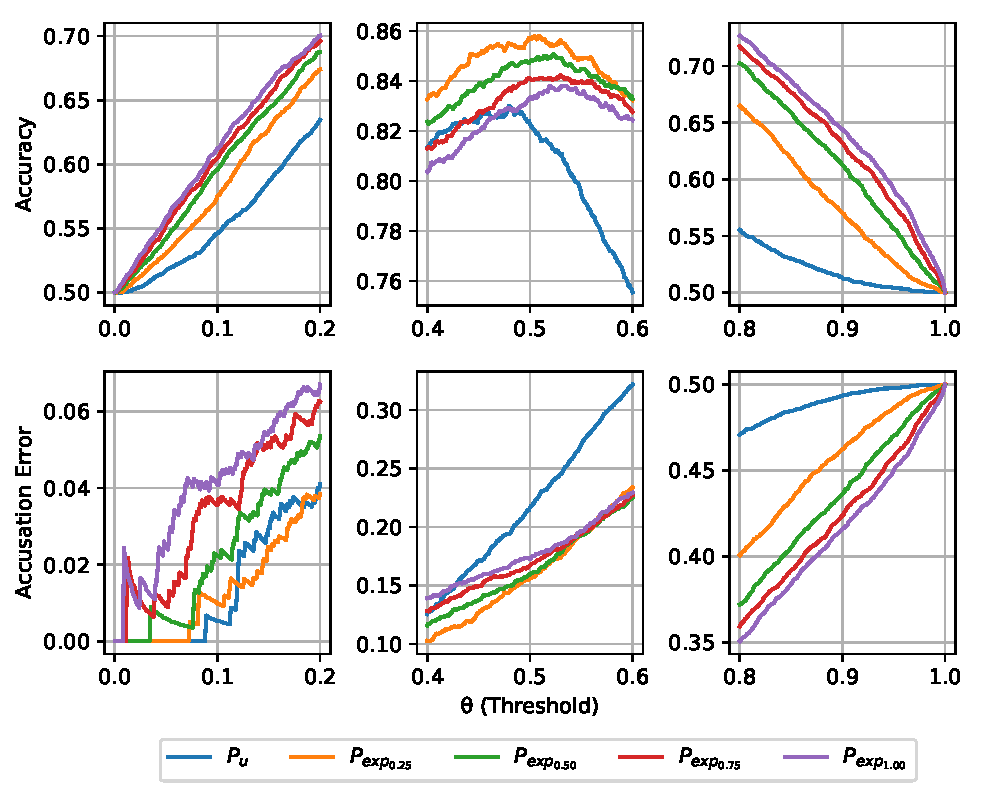
\includegraphics[width=0.7\textwidth]{./pictures/discussion/conv_char_nn_prediction_zoom_50_time}
            \caption{Illustrate important intervals for our different
                $P_{exp_\lambda}$ prediction systems for the \gls{conv-char-NN}
                network on the dataset with 50\% negative samples. On the left
                we have shown the beginning of the curves, in the middle we have
                shown the top accuracy and to the right we have shown the end of
                the curves.}
            \label{fig:conv_char_prediction_zoom_50}
        \end{figure}

    \item[$\mathbf{P_l}$]

        The idea behind the length based prediction system was that
        longer texts would better reflect the writing style of an
        author. Some of the texts in the dataset are only a few hundred
        characters long which means that only few of the n-grams the
        networks are looking for will be present in those texts. In Figure
        \ref{fig:conv_char_prediction_zoom_50_text_length} we have shown a
        comparison between $P_\mathcal{U}$ and $P_l$. It can be seen there that
        it is always better to weight based on text length than it is to just
        use uniform weights. The curves follow each other closely but $P_l$
        have slightly higher accuracy and slightly lower accusation error than
        $P_\mathcal{U}$. That is exactly the result we expected and shows that
        it was a good idea to look at text length as part of our prediction
        systems.

        \begin{figure}
            \centering
            \textbf{$\mathbf{P_l}$ \& $\mathbf{P_{lexp_{0.25}}}$ \&
            $\mathbf{P_{exp_{0.25}}}$ 0.5 Split}\par\medskip
            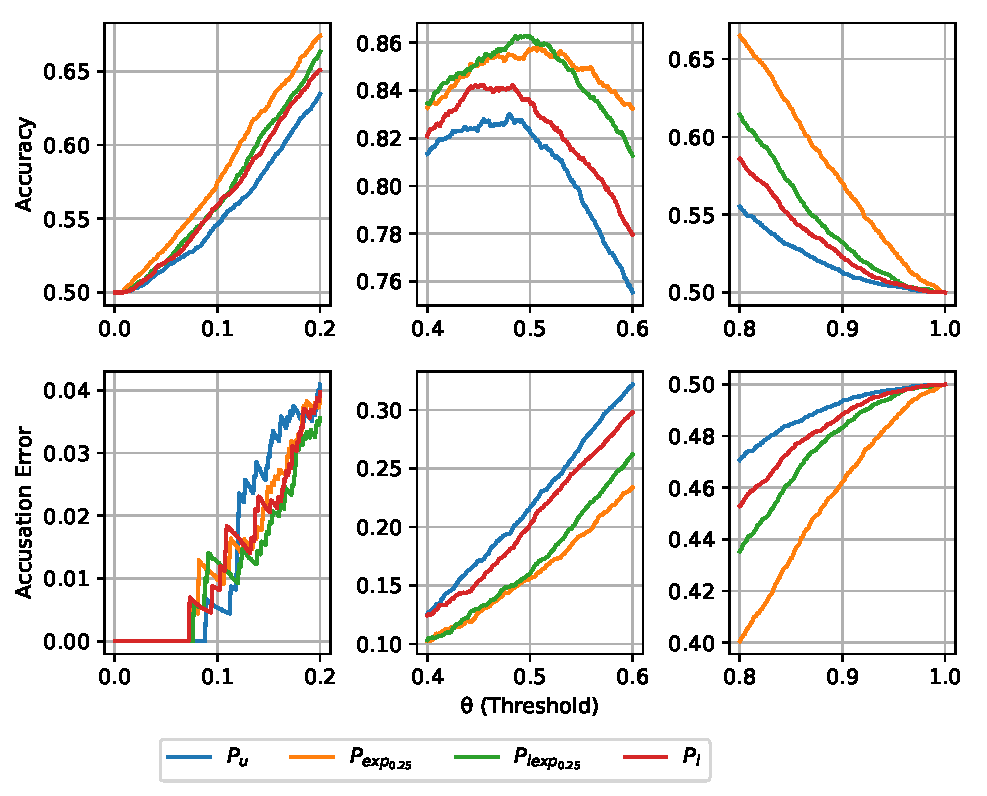
\includegraphics[width=0.7\textwidth]{./pictures/discussion/conv_char_nn_prediction_zoom_length}
            \caption{Illustrate important intervals for our $P_l$,
                $P_{exp_\lambda}$ and $P_{lexp_{\lambda}}$ prediction systems
                for the \gls{conv-char-NN} network on the 0.5 split dataset. On
                the left we have shown the beginning of the curves, in the
                middle we have shown the top accuracy and to the right we have
                shown the end of the curves.}
            \label{fig:conv_char_prediction_zoom_50_text_length}
        \end{figure}

    \item[$\mathbf{P_{lepx_{0.25}}}$]

        This prediction system were a combination of the time based and text
        length based prediction systems. Multiple different networks had this
        configuration as the configuration that maximized accuracy. We have
        already concluded that both $P_l$ and $P_{exp_\lambda}$ was better
        weightings than $P_\mathcal{U}$. So the interesting thing about this
        weight is not whether or not it beats $P_\mathcal{U}$, but rather
        whether or not it is better than $P_l$ and $P_{exp_\lambda}$. In Figure
        \ref{fig:conv_char_prediction_zoom_50_text_length} we have shown the
        performance of $P_{lexp_\lambda}$ vs some similar prediction systems.

        In that Figure we see that $P_{exp_{0.25}}$ has generally better
        performance than $P_{lexp_{0.25}}$ except right at the maximum accuracy.
        At the maximum accuracy $P_{lexp_{0.25}}$ is able to just barely beat
        $P_{exp_{0.25}}$. Almost all the networks used the $P_{lexp_{0.25}}$
        prediction system as the best prediction system and it must be this
        small difference that causes that.

    \item[$\mathbf{P_{MV}}$]

        The majority vote prediction system $P_{MV}$ is similar to the uniform
        prediction system $P_{\mathcal{U}}$. We therefore expected about similar
        performance. We have shown the $P_{MV}$ prediction systems performance
        in Figure \ref{fig:conv_char_prediction_zoom_50_majority_vote}. It is
        clear in that figure that $P_{MV}$ has almost the same performance as
        the uniform weighing. The curves follow each other closely however the
        $P_\mathcal{U}$ prediction system has slightly higher performance at the
        top of the curves.

        \begin{figure}
            \centering
            \textbf{$\mathbf{P_{MV}}$ \& $\mathbf{P_{min}}$ \&
            $\mathbf{P_{max}}$ 0.5 Split}\par\medskip
            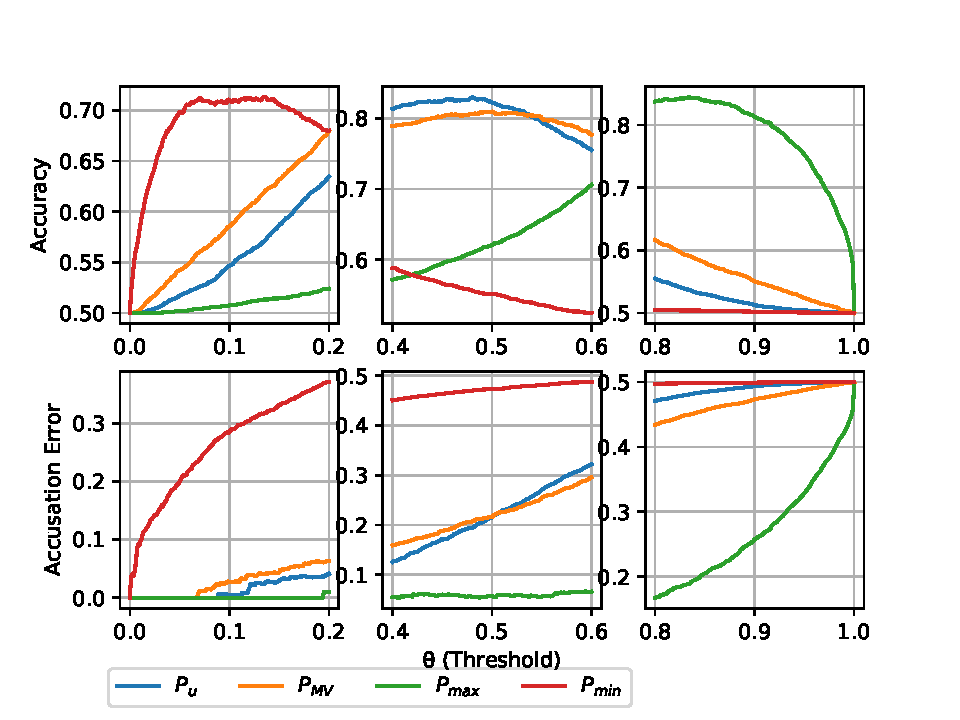
\includegraphics[width=0.7\textwidth]{./pictures/discussion/conv_char_nn_prediction_zoom_min_max}
            \caption{Illustrate important intervals for our $P_{MV}$, $P_{max}$
                and $P_{min}$ prediction systems for the \gls{conv-char-NN}
                network on the 0.5 split dataset. On the left we have shown the
                beginning of the curves, in the middle we have shown the top
                accuracy and to the right we have shown the end of the curves.}
            \label{fig:conv_char_prediction_zoom_50_majority_vote}
        \end{figure}

    \item[$\mathbf{P_{min}}$]

        The $P_{min}$ system is the only prediction system with worse
        performance than the $P_{\mathcal{U}}$ system. The problem is that
        the accusation error rise very quickly. Even though the accuracy
        also rise quickly the accusation error rises so quickly that the
        systems thresholds give to high accusation error to be used. We
        can also see that the maximum accuracy of the $P_{min}$ system
        is around 70\% which is also lower than the other systems. We
        have shown a plot of the $P_{min}$ prediction system in Figure
        \ref{fig:conv_char_prediction_zoom_50_majority_vote}.

    \item[$\mathbf{P_{max}}$]

        The maximum prediction system reaches maximum accuracy
        later than any other prediction system. We have shown a
        Figure comparing the system to other systems in Figure
        \ref{fig:conv_char_prediction_zoom_50_majority_vote}. The accusation
        error of the system stays low for higher $\theta$s than any other
        prediction system. Unfortunately the accuracy also rises slowly. We had
        expected that the maximum prediction system would have a low accusation
        error as it only looked at the single text in an authors library most
        similar to an text of unknown authorship.

\end{description}

To summarize we find that the prediction systems with the best performance are
generally the time based prediction systems. It was expected from the findings
of \citet{hansen2014} that the turn in time of an text is an important factor.
We also find that the length of the text is also an important factor and in most
cases we see that the best prediction system is the system that is a combination
of time and text length. More of an authors writing style will be represented in
longer texts so it makes sense that longer texts should be weighted higher.


\subsection{Writing Style Changes}
\label{subsec:writing_style_changes}

In this section we discuss how a secondary school students writing style changes
during his/her school years. We observed that time based weights worked well
when doing authorship verification. That suggests that there is some development
in students writing style which would also be expected. Secondary school is
probably one of the time periods writing style changes the most.

\begin{figure}
    \centering
    \textbf{Writing Style Changes}\par\medskip
    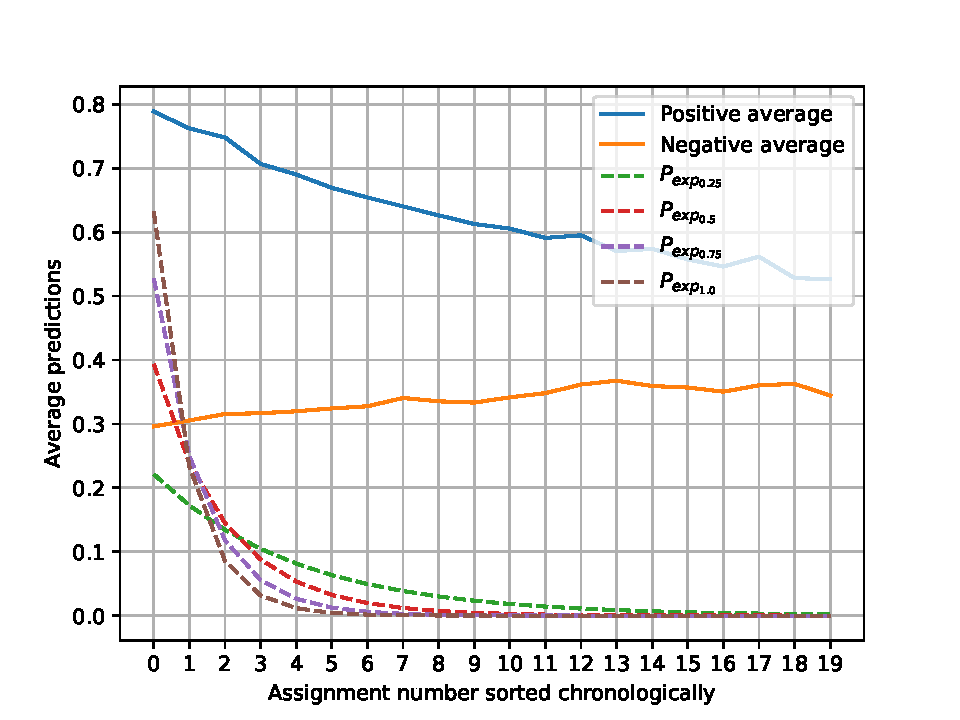
\includegraphics[width=0.7\textwidth]{./pictures/discussion/writing_style_change}
    \caption{Average predictions of newest to oldest texts for positive samples
        and negative samples by the \gls{conv-char-NN}. The newest text is shown
        to the left and the oldest to the right. We have also shown a plot of
        the different time based weight functions we tried using.}
    \label{fig:writing_style_changes}
\end{figure}

To get an idea of how much the writing style of a student changes over time we
looped through each author in the \gls{D} dataset. We created a positive and a
negative sample for each of the authors and used \gls{conv-char-NN} to predict
each of the authors texts against the positive and negative sample. We then
computed the average score of the newest text, the average score of the second
newest text, and so on for both positives and negatives. If the students writing
style changes over time we would expect the newest text having an higher average
score than the oldest texts for the positive samples. We also expect that the
negative samples are to have an average of less then 0.5 but about the same
for each text. In Figure \ref{fig:writing_style_changes} we have illustrated
the average positive and negative predictions produced by our network. We only
predict the newest 20 texts as very few authors in the dataset has more than
that. So the averages of the texts above 20 vary wildly.

In that figure it is very clear that writing style does change over time. The
positive samples fall from 80\% average similarity on the newest assignment to
just over 50\% on the oldest assignment. That is a very large drop that suggests
that after only 20 turn ins the writing style has changed so drastically that
our network almost believes it is someone else. It is very interesting that the
drop in accuracy seem to follow closely our $P_{exp_{0.25}}$ prediction system
weights. That is probably the reason why that particular $\lambda$ value for the
time based prediction systems so often gave the best results.

The negative curve is a bit weird. We expected it to stay flat below 50\% but
it seems to be rising towards 50\%. It only rises slowly towards 50\%. Much
slower than the positive curve falls. While the positive curve drops almost 30
points the negative curve only rises 5. It might be just a coincidence.


\subsection{Features}

In this section we will discuss the features our best network
(\gls{conv-char-NN}) seem to be extracting and using for classification. It is
interesting which kinds of features the network use to represent the texts. That
information can be used to design new network architectures or to inspire manual
feature selections. We have identified several different classes of features the
network is looking at:

\begin{description}
    \item[Abbreviations]

        Examples of filters looking for \textit{abbreviation features} are,

        ``\verb|ag, pga.|'', ``\verb|a. bl.a.|'', ``\verb|Fx. |'',
        ``\verb|om fx ""|'' and ``\verb|, F.eks.|''.

        The first category of features we noticed were features looking for
        abbreviations. It makes sense for the network to look at the different
        abbreviations used by an author. An author will probably keep using
        the same abbreviations and it will therefore be an excellent feature
        for distinguishing between different authors. Some authors will write
        out their phrases and will not use abbreviations. The first example
        above looks for an abbreviations that means ``because of'' and the
        second means ``among other''. The last three examples is of special
        interest they all mean the same thing, ``for example'', but represent
        different ways of abbreviating that. Some authors will use the first
        style, some the second, some the third and some will write it out as
        ``for eksempel''.

    \item[Start of Sentences]

        Examples of filters looking for \textit{start of sentence features} are,

        ``\verb|Måsk|'', ``\verb| Hvilket|'', ``\verb|Samtidig|'',
        ``\verb|x. Men h|'' and ``\verb|. Her ef|''.

        The filters above all look for specific words used in the beginning of
        a sentence. Different authors has a tendency to start sentences with
        different words so it makes sense to look at the beginning of sentences
        when verifying authorship. The filters above means ``Maybe'', ``Which'',
        ``At the same time'', ``But'' and ``After that'' respectively.

    \item[Style]

        Examples of filters looking for \textit{style features} are,

        ``\verb| 2 af 2"|'', ``\verb|\nPAGE\n\n4|, ``\verb|siger: “|'',
        ``\verb|såsom ’’|'', ``\verb|t” dette|'', ``\verb|’’ \nSide|'' and
        ``\verb|at.dk/\n\n|''.

        The first two filters reacts to different footer styles. The first
        footer style is activated when authors write their page numbering as
        ``2 of 2'' while the second style is activated when authors write their
        page numbering as ``PAGE\textbackslash n\textbackslash n2''. It is
        interesting that the network has been able to learn from the footers
        of the documents and not just from body text. It is clear to us that
        authors will generally use he same footer style in all their texts. The
        footer style is probably dictated mainly by the program they use to
        write the texts.

        The next two filters reacts to different citation styles. The first
        one reacts to citations such as ``the author says: "<citation>'' and
        the second reacts to citations such as ``as "<citation>''. Again it is
        interesting that the network has learned that some authors will have a
        tendency to cite in a specific way while others do not.

        The next two filters reacts to styles used after citations. The first
        of them reacts to styles such as ``<citation>" this shows that'' while
        the second contains what looks like a reference to a page number of
        the citation, such as in ``<citation>" \textbackslash nPage 5''. It is
        probably mostly the teacher that determines whether or not students
        will write page numbers for their citations. Some teachers will require
        page numbering while others will not. A ghostwriter might not know the
        citation style the student normally use and use something else.

        The last filter seems to look at links in footers. It reacts to links
        followed by two newlines.

    \item[Vocabulary]

        Examples of filters looking for \textit{vocabulary features} are,

        ``\verb| mandig,|'', ``\verb|, mens ’|'', ``\verb|r dog kr|'',
        ``\verb|forsøger|'', ``\verb|ademisk,|'' and ``\verb|r altså\n|''.

        All these filters react to specific words. The words are translated
        ``manly'', ``while'', ``however'', ``try'', ``academic'' and ``so''. The
        texts in the dataset we use are generally short so these words will not
        occur in all texts. The presence of specific words in an assignment will
        clearly indicate specific authors. Some of the words above has synonyms
        so an author can choose between which synonym to use. Others are just
        words that rarely occurs in a text but might be more likely to be used
        by certain authors than others.

    \item[Unknown]

        Examples of filters that looks at \textit{unknown features} are,

        ``\verb|!’’.|'', ``\verb| '” d" '|'' and ``\verb|–\n\nf|''.

        These are examples of features that are hard to parse. It might be
        the case that these filters look at some sort of punctuation. The
        reason the maximum activations looks so weird could then be because the
        maximum activations come from some of the corrupted assignments in the
        dataset. So it might be that on normal texts these filters are useful to
        determine the punctuation style of authors.

        Another possibility is that they react to artifacts left over from the
        text extraction from pdfs. It might be that some students use specific
        programs that generate pdfs where when text is extracted from them
        generate weird sequences of characters. That could of course be used to
        identify students and might even work well since ghostwriters might use
        another program. However it does not seem like a good thing for the
        network to look at.

\end{description}

We believe our network has learned interesting and useful features. The
description above shows that the network has learned several different kinds
of features and there are probably many more that we missed. Features in
classical authorship verification are as described earlier often frequencies
\citep{stamatos2009}. That is in contrast to our features which represents the
presence of a certain character sequence. That means that our networks are able
to look at things that would not have been possible with a frequency such as the
style of footers and style of citations. Classical features has an advantage
in that they give information not only on presence but how often a character
sequence is used. It would have been interesting to train a network that
contained constructs for extracting frequencies (for example by using average
pooling) and the current constructs for extracting presence. Then the dense
network could use both of those different kinds of features to make predictions.

    \FloatBarrier

    \section{Conclusion} \label{sec:conclusion}

We have created three deep neural networks. The networks works on different
layers of an authors texts. The character layer, the word layer and the sentence
layer. We evaluated all networks on a dataset with 96\% positive cases and
4\% negative cases. That split reflects the believed real world data. On
that test dataset all of our networks performed better than the baseline
methods. Furthermore one of our networks \gls{conv-char-NN} had slightly better
performance than previous work on MaCom's dataset that we have found.

We did not hit the targets set by MaCom at the beginning of the project. The
specifications were to have an accusation error below 10\% and still catch 95\%
of the cheaters. We knew that that goal was very ambitious and we focused on
fulfilling the first requirement. We ended up with an accusation error of 23\%
and caught 8.5\% of the cheaters on our best network. The fact that we used a
dataset with only 4\% negatives made it very hard to keep the accusation error
low.

We looked at what kind of feedback we could give to teachers. We found that it
is possible for some of our networks to report the largest differences between
the texts. A teacher would be able to use thousands of those differences
to explain why an assignment might be ghost written. We also performed an
experiment that showed that we are able to find the areas of a text most likely
to be ghost written. The results were not overwhelmingly positive as the
difference between ghost written and non ghost written paragraphs were small.
That suggests that our networks has problems handling such small amounts of
text.

We believe that the networks we have implemented are not ready to be implemented
in a real world setting. However we also believe that it is possible to continue
working with the methods we have explored and obtain something that is ready for
implementation. We have used previous work on MaCom's datasets as a starting
point for our own methods. Similarly future work on the dataset might be based
on the work in this thesis.

We have shown by beating our baselines and getting slightly better results on
previous work on MaCom's dataset that it is possible to use neural networks
on raw text data when performing authorship verification. One of the big
advantages of our methods is that the input to the network is raw text. There
is no need for manual feature engineering as classic authorship attribution and
verification requires. Another big advantage is that our model is generalizing.
It can be trained once and used many times. As explained before classifying
a single text is fast and classifying $n$ texts is very parallelizable.
The classification of a single text contains no dependencies on any other
classifications and can therefore be performed on arbitrarily many machines.

    \FloatBarrier

    \section{Future Work} \label{sec:future_work}

A concern brought up in Section \ref{subsec:applicability_of_method} regard
the applicability of our current methods to other courses or other types of
text data like code. It would be interesting to apply our methods to texts from
other secondary school courses and observe the performance. It would also be
interesting to apply the methods to other age classes such as primary school
students or college students. Application to primary school students might be
hard since assignments are typically shorter and writing style might change even
more than during secondary school. However application to college students might
lead to very encouraging results since writing style probably remains more fixed
and assignments are generally longer.

Another concern brought in Section \ref{subsec:applicability_of_method}, was
the inclusion of citation in the texts provided to our models. Citation are
mostly a source of noise for our models. This makes the most sensible solution
when working with these models in future to simply remove the citations before
training and applying the methods. Doing so successfully might increase the
accuracy of our models further.

There is also the scenario where a group of students do a collective handin of a
collaborative assignment. As mentioned in Section \ref{subsubsec:group_handin}
this is not something that our methods would be able to handle out of the box.
However a future modification of our methods could tackle this using a paragraph
based approach. As described in Section \ref{subsubsec:ghost_written_areas} one
could loop through each paragraph in the collaborative text, and then apply
our methods. The paragraph would be tested against all the students who worked
on the assignment. The goal would be to attribute each paragraph to one of the
proposed writers of the assignment. If a certain amount of paragraphs were
unattributable then the entire text would be considered the product of a ghost
writer. In this scenario a subset of student in the group might have had their
parts produced by a third party ghost writer.

A big focus during our experiments was keeping the model generalizing, and
not author specific. Future work could include verifying the reach of this
generalizability. Our primary concern was the generalizability with regard to
secondary school students, but what if the generalizability extends to a larger
group of authors than that. This would mean the model was more powerful than
originally thought, thus expanding the areas of usability quite a bit. Tests
of this could include applying the our models to another dataset. This could
be anything from scientific papers to newspaper articles, anything where the
author has a substantial amount of work behind him.

As we briefly mentioned in Section \ref{subsec:writing_style_changes} students
writing style can be seen to change over time. It would be interesting to study
exactly what changes occur. That might lead to insights into teaching methods.
We could also look at finding students with little writing style development and
flagging them as needing extra help from teachers.

    \FloatBarrier

    \bibliographystyle{apalike}
    \bibliography{literature}

    \newpage
    \appendix
    \section{Appendix}

\subsection{Computer Specifications}
\verbinput{./data/DxDiag.txt}

\subsection{Training Data Statistics}\label{sec:B_stats}
\verbinput{./data/b_stata.txt}

\subsection{Extended Delta Feature Selection}\label{sec:ed_feat}
\begin{center}
\begin{tabular}{ccc}
Feature Type & Frequency Rank & Feature \\ \hline
Char 4 Gram & 58 & ', og'\\
Char 5 Gram & 3 & ', at '\\
Char 5 Gram & 16 & ', der'\\
Char 7 Gram & 42 & 'politik'\\
Char 10 Gram & 269 & ' naturligv'\\
Char 4 Gram & 256 & 'e er'\\
Char 2 Gram & 34 & '. '\\
Word 4 Gram & 266 & ('jeg', 'vil', 'gerne', 'have')\\
Char 10 Gram & 275 & 'myndighede'\\
Char 10 Gram & 29 & ' Europa-Pa'\\
\end{tabular}
\end{center}

\subsection{SVM Feature Selection}\label{sec:svm_feat}
\begin{center}
\begin{tabular}{ccc}
Feature Type & Frequency Rank & Feature \\ \hline
Char 5 Gram & 13 & ', som'\\
Char 3 Gram & 136 & ', o'\\
Char 3 Gram & 53 & ', a'\\
Char 7 Gram & 199 & 'er sig '\\
Char 6 Gram & 2 & ', der '\\
Char 7 Gram & 191 & ' ændrin'\\
Word 3 Gram & 397 & ('tager', 'hensyn', 'til')\\
Char 4 Gram & 51 & ', so'\\
Char 10 Gram & 187 & ' medlemmer'\\
Word 2 Gram & 346 & ('princippet', 'om')\\
Word 3 Gram & 352 & ('og', 'vi', 'vil')\\
Word 3 Gram & 2 & ('med', 'hensyn', 'til')\\
Char 6 Gram & 130 & ' alle '\\
Char 8 Gram & 186 & ' for det'\\
Char 7 Gram & 180 & 'ngen af'\\
Char 5 Gram & 297 & 'er vi'\\
Char 5 Gram & 143 & 'orsla'\\
Word 4 Gram & 255 & ('som', 'jeg', 'gerne', 'vil')\\
Char 9 Gram & 83 & ' hensyn t'\\
Word 2 Gram & 358 & ('det', 'vi')\\
Char 7 Gram & 39 & 'der er '\\
Word 4 Gram & 329 & ('p', 'en', 'eller', 'anden')\\
Char 4 Gram & 124 & ', hv'\\
Char 8 Gram & 169 & 'amarbejd'\\
Char 4 Gram & 38 & ' om '\\
Word 4 Gram & 409 & ('er', 'ndvendige', 'for', 'at')\\
Char 5 Gram & 178 & 'eres '\\
Char 4 Gram & 121 & 'e af'\\
Char 7 Gram & 258 & 'er den '\\
Char 4 Gram & 49 & 'ring'\\
Char 5 Gram & 97 & 'lamen'\\
Word 4 Gram & 400 & ('forhandling', 'under', 't', 'om')\\
Char 10 Gram & 289 & ' drejer si'\\
Char 4 Gram & 168 & ' ogs'\\
Char 8 Gram & 151 & 'ndelse m'\\
Char 7 Gram & 189 & ' som de'\\
Word Gram & 223 & 'naturligvis'\\
Char 4 Gram & 185 & 'erin'\\
Char 4 Gram & 241 & 'rer '\\
Char 5 Gram & 107 & 'til a'\\
Char 9 Gram & 104 & ' økonomis'\\
Char 6 Gram & 183 & 'ndling'\\
Char 9 Gram & 75 & 'gsforslag'\\
Char 4 Gram & 234 & 'denn'\\
Char 6 Gram & 78 & 'or at '\\
Char 8 Gram & 4 & 'issionen'\\
Char 5 Gram & 280 & ' arbe'\\
Char 9 Gram & 23 & 'Hr. forma'\\
Word Gram & 239 & 'medlemmer'\\
Char 5 Gram & 204 & 'lande'\\
Word 3 Gram & 290 & ('i', 'de', 'seneste')\\
Word 3 Gram & 381 & ('i', 'dag', 'har')\\
Char 9 Gram & 86 & 'ællesskab'\\
Char 9 Gram & 9 & 'uropæiske'\\
Char 10 Gram & 191 & ', hvilket '\\
Char 3 Gram & 212 & 'igh'\\
Char 10 Gram & 78 & 'ndringsfor'\\
Char 8 Gram & 97 & ' kommiss'\\
Char 9 Gram & 266 & 'sige, at '\\
Char 9 Gram & 39 & '. Hr. for'\\
Char 4 Gram & 266 & ' und'\\
Char 9 Gram & 8 & 'issionen '\\
Char 4 Gram & 171 & 'orma'\\
Char 5 Gram & 101 & ' dett'\\
Char 8 Gram & 157 & 'rhandlin'\\
Word 4 Gram & 335 & ('konomisk', 'og', 'social', 'samhrighed')\\
Char 6 Gram & 245 & 'beslut'\\
Char 7 Gram & 269 & 'er skal'\\
Word Gram & 369 & 'ligeledes'\\
Word 4 Gram & 191 & ('nr', 'det', 'handler', 'om')\\
Char 9 Gram & 296 & 'grund af '\\
Char 4 Gram & 37 & ', de'\\
Char 3 Gram & 278 & 'lde'\\
Word 2 Gram & 486 & ('min', 'gruppe')\\
Char 9 Gram & 192 & 'offentlig'\\
\end{tabular}
\end{center}

\subsection{Convolution	Filters}
\begin{table}
    \centering
    \textbf{Convolutional Filter 1 of Size 8}\par\medskip
    \begin{tabular}{c|cc}
        & \textbf{Filter Max String} & \textbf{Filter Max Value} \\ \hline
        \textbf{Text 13}  & \verb{', så at '{  & 44.41869 \\
        \textbf{Text 49}  & \verb{'2 se at '{  & 42.97375 \\
        \textbf{Text 29}  & \verb{'omas at '{  & 42.86139 \\
        \textbf{Text 21}  & \verb{'n nå at '{  & 42.27350 \\
        \textbf{Text 48}  & \verb{'r så at '{  & 41.95458 \\
        \textbf{Text 20}  & \verb{', nu et '{  & 41.92461 \\
        \textbf{Text 26}  & \verb{'t se at '{  & 41.03944 \\
        \textbf{Text 17}  & \verb{'m af at '{  & 40.85154 \\
        \textbf{Text 10}  & \verb{'mene at '{  & 40.75563 \\
        \textbf{Text 16}  & \verb{'mene at '{  & 40.75563 \\
        \textbf{Text 27}  & \verb{' bar at '{  & 40.46385 \\
        \textbf{Text 6}   & \verb{'r os at '{  & 40.32341 \\
        \textbf{Text 42}  & \verb{' tid at '{  & 39.77865 \\
        \textbf{Text 30}  & \verb{'også at '{  & 39.58638 \\
        \textbf{Text 36}  & \verb{'også at '{  & 39.58638 \\
        \textbf{Text 40}  & \verb{'r nu et '{  & 39.46050 \\
        \textbf{Text 9}   & \verb{'n af at '{  & 39.40045 \\
        \textbf{Text 32}  & \verb{'n af at '{  & 39.40045 \\
        \textbf{Text 41}  & \verb{'n af at '{  & 39.40045 \\
        \textbf{Text 46}  & \verb{'n af at '{  & 39.40045 \\
        \textbf{Text 1}   & \verb{'ådan at '{  & 39.32121 \\
        \textbf{Text 12}  & \verb{', er et '{  & 39.25355 \\
        \textbf{Text 43}  & \verb{', er et '{  & 39.25355 \\
        \textbf{Text 14}  & \verb{'ldes at '{  & 38.98859 \\
        \textbf{Text 24}  & \verb{'rlag at '{  & 38.83994 \\
        \textbf{Text 15}  & \verb{'g af at '{  & 38.72359 \\
        \textbf{Text 38}  & \verb{'” er at '{  & 38.71601 \\
        \textbf{Text 33}  & \verb{'n på at '{  & 38.57942 \\
        \textbf{Text 18}  & \verb{'t er at '{  & 38.56930 \\
        \textbf{Text 34}  & \verb{'r på at '{  & 38.48225 \\
        \textbf{Text 45}  & \verb{'r på at '{  & 38.48225 \\
        \textbf{Text 4}   & \verb{'vder at '{  & 38.43643 \\
        \textbf{Text 5}   & \verb{'vder at '{  & 38.43643 \\
        \textbf{Text 3}   & \verb{'r vi at '{  & 38.40871 \\
        \textbf{Text 19}  & \verb{'yder at '{  & 38.40115 \\
        \textbf{Text 25}  & \verb{'yder at '{  & 38.40115 \\
        \textbf{Text 37}  & \verb{'nder at '{  & 38.37101 \\
        \textbf{Text 11}  & \verb{'ømme at '{  & 38.25414 \\
        \textbf{Text 39}  & \verb{'s af at '{  & 38.21890 \\
        \textbf{Text 23}  & \verb{' var at '{  & 38.07627 \\
        \textbf{Text 7}   & \verb{'sted at '{  & 37.97903 \\
        \textbf{Text 47}  & \verb{'fter at '{  & 37.91461 \\
        \textbf{Text 28}  & \verb{'gter at '{  & 37.87117 \\
        \textbf{Text 8}   & \verb{'d af at '{  & 37.70177 \\
        \textbf{Text 35}  & \verb{' til at '{  & 37.03082 \\
        \textbf{Text 44}  & \verb{' til at '{  & 37.03082 \\
        \textbf{Text 22}  & \verb{'n er et '{  & 36.88660 \\
        \textbf{Text 2}   & \verb{' dag i t'{  & 26.28683 \\
        \textbf{Text 31}  & \verb{'· Frank\n'{ & 21.83477
    \end{tabular}
    \caption{The most important part of the first 50 texts according to
        convolutional filter 1 of size 8. Sorted by the importance score.}
    \label{fig:features_convolution_8_1}
\end{table}

\begin{table}
    \centering
    \textbf{Convolutional Filter 5 of Size 8}\par\medskip
    \begin{tabular}{c|cc}
        & \textbf{Filter Max String} & \textbf{Filter Max Value} \\ \hline
        \textbf{Text 3} & \verb{' meget k'{ & 18.73260 \\
        \textbf{Text 10} & \verb{' meget k'{ & 18.73260 \\
        \textbf{Text 13} & \verb{' meget k'{ & 18.73260 \\
        \textbf{Text 15} & \verb{' meget k'{ & 18.73260 \\
        \textbf{Text 21} & \verb{' meget k'{ & 18.73260 \\
        \textbf{Text 24} & \verb{' meget k'{ & 18.73260 \\
        \textbf{Text 29} & \verb{' meget k'{ & 18.73260 \\
        \textbf{Text 32} & \verb{' meget k'{ & 18.73260 \\
        \textbf{Text 33} & \verb{' meget k'{ & 18.73260 \\
        \textbf{Text 9} & \verb{' meget g'{ & 18.71884 \\
        \textbf{Text 20} & \verb{' meget g'{ & 18.71884 \\
        \textbf{Text 26} & \verb{' meget g'{ & 18.71884 \\
        \textbf{Text 17} & \verb{' meget s'{ & 18.39024 \\
        \textbf{Text 22} & \verb{' meget s'{ & 18.39024 \\
        \textbf{Text 23} & \verb{' meget s'{ & 18.39024 \\
        \textbf{Text 27} & \verb{' meget s'{ & 18.39024 \\
        \textbf{Text 28} & \verb{' meget s'{ & 18.39024 \\
        \textbf{Text 30} & \verb{' meget s'{ & 18.39024 \\
        \textbf{Text 42} & \verb{' meget s'{ & 18.39024 \\
        \textbf{Text 46} & \verb{' meget s'{ & 18.39024 \\
        \textbf{Text 47} & \verb{' meget s'{ & 18.39024 \\
        \textbf{Text 36} & \verb{' benytte'{ & 18.37530 \\
        \textbf{Text 37} & \verb{' benytte'{ & 18.37530 \\
        \textbf{Text 40} & \verb{' benytte'{ & 18.37530 \\
        \textbf{Text 8} & \verb{' meget n'{ & 17.72581 \\
        \textbf{Text 16} & \verb{' meget n'{ & 17.72581 \\
        \textbf{Text 14} & \verb{' kendt s'{ & 17.69235 \\
        \textbf{Text 18} & \verb{' kendt s'{ & 17.69235 \\
        \textbf{Text 7} & \verb{' meget i'{ & 17.64814 \\
        \textbf{Text 25} & \verb{' taget g'{ & 17.53552 \\
        \textbf{Text 1} & \verb{' blidt k'{ & 17.45398 \\
        \textbf{Text 5} & \verb{'rkendt s'{ & 17.40653 \\
        \textbf{Text 12} & \verb{' meget r'{ & 17.39020 \\
        \textbf{Text 4} & \verb{' taget s'{ & 17.20692 \\
        \textbf{Text 48} & \verb{' faldt i'{ & 17.18553 \\
        \textbf{Text 44} & \verb{'åkaldt k'{ & 16.80688 \\
        \textbf{Text 38} & \verb{'rne om k'{ & 16.71076 \\
        \textbf{Text 49} & \verb{' Blod,fr'{ & 16.50881 \\
        \textbf{Text 39} & \verb{' stolthe'{ & 16.18284 \\
        \textbf{Text 34} & \verb{'vilket k'{ & 16.07917 \\
        \textbf{Text 43} & \verb{'vilket k'{ & 16.07917 \\
        \textbf{Text 41} & \verb{'vilket g'{ & 16.06541 \\
        \textbf{Text 45} & \verb{' herefte'{ & 15.82326 \\
        \textbf{Text 35} & \verb{'-oprette'{ & 15.73831 \\
        \textbf{Text 31} & \verb{'rndommen'{ & 15.38827 \\
        \textbf{Text 6} & \verb{' sendt i'{ & 15.38613 \\
        \textbf{Text 11} & \verb{'’opret n'{ & 15.11496 \\
        \textbf{Text 19} & \verb{'rne om f'{ & 14.34204 \\
        \textbf{Text 2} & \verb{' betydni'{ & 13.36254 \\
    \end{tabular}
    \caption{The most important part of the first 50 texts according to
        convolutional filter 5 of size 8. Sorted by the importance score.}
    \label{fig:features_convolution_8_5}
\end{table}

\begin{table}
    \centering
    \textbf{Convolutional Filter 100 of Size 8}\par\medskip
    \begin{tabular}{c|cc}
        & \textbf{Filter Max String} & \textbf{Filter Max Value} \\ \hline
        \textbf{Text 20} & \verb{', at De '{ & 14.06486 \\
        \textbf{Text 3} & \verb{', at de '{ & 13.97819 \\
        \textbf{Text 5} & \verb{', at de '{ & 13.97819 \\
        \textbf{Text 21} & \verb{', at de '{ & 13.97819 \\
        \textbf{Text 24} & \verb{', at de '{ & 13.97819 \\
        \textbf{Text 25} & \verb{', at de '{ & 13.97819 \\
        \textbf{Text 40} & \verb{'– \nFælle'{ & 13.60728 \\
        \textbf{Text 27} & \verb{', at der'{ & 13.18669 \\
        \textbf{Text 32} & \verb{', at der'{ & 13.18669 \\
        \textbf{Text 43} & \verb{', at der'{ & 13.18669 \\
        \textbf{Text 39} & \verb{'– ”hele '{ & 12.20550 \\
        \textbf{Text 1} & \verb{', klædt '{ & 12.14879 \\
        \textbf{Text 10} & \verb{', havde '{ & 11.90384 \\
        \textbf{Text 11} & \verb{', havde '{ & 11.90384 \\
        \textbf{Text 16} & \verb{', burde '{ & 11.81674 \\
        \textbf{Text 13} & \verb{', at vi '{ & 11.33311 \\
        \textbf{Text 23} & \verb{', at vi '{ & 11.33311 \\
        \textbf{Text 30} & \verb{', at vi '{ & 11.33311 \\
        \textbf{Text 19} & \verb{'– Sorte '{ & 11.28722 \\
        \textbf{Text 29} & \verb{'– altid '{ & 11.25181 \\
        \textbf{Text 6} & \verb{', hf og '{ & 11.11696 \\
        \textbf{Text 17} & \verb{', Fauli '{ & 10.95995 \\
        \textbf{Text 4} & \verb{', IB og '{ & 10.94379 \\
        \textbf{Text 33} & \verb{', og de '{ & 10.79599 \\
        \textbf{Text 35} & \verb{', og de '{ & 10.79599 \\
        \textbf{Text 48} & \verb{', og de '{ & 10.79599 \\
        \textbf{Text 26} & \verb{', EF og '{ & 10.68619 \\
        \textbf{Text 22} & \verb{'– eller '{ & 10.67318 \\
        \textbf{Text 38} & \verb{'– eller '{ & 10.67318 \\
        \textbf{Text 15} & \verb{', da de '{ & 10.57667 \\
        \textbf{Text 9} & \verb{', fordi '{ & 10.42775 \\
        \textbf{Text 12} & \verb{', fordi '{ & 10.42775 \\
        \textbf{Text 18} & \verb{', grund;'{ & 10.22946 \\
        \textbf{Text 8} & \verb{'n at de '{ & 10.03539 \\
        \textbf{Text 34} & \verb{', at jo '{ & 10.00943 \\
        \textbf{Text 46} & \verb{'øget og '{ & 9.95325 \\
        \textbf{Text 28} & \verb{'– en opl'{ & 9.85135 \\
        \textbf{Text 7} & \verb{'\n\n\nLader'{ & 9.81295 \\
        \textbf{Text 37} & \verb{', da der'{ & 9.78517 \\
        \textbf{Text 41} & \verb{'\n\n\nHele '{ & 9.64712 \\
        \textbf{Text 49} & \verb{'\n\n\nHele '{ & 9.64712 \\
        \textbf{Text 47} & \verb{', impres'{ & 9.57604 \\
        \textbf{Text 14} & \verb{'ørte en '{ & 9.50064 \\
        \textbf{Text 44} & \verb{', Fædrel'{ & 9.32844 \\
        \textbf{Text 42} & \verb{', at jor'{ & 9.21792 \\
        \textbf{Text 45} & \verb{'\n\n\n\nDet '{ & 8.97469 \\
        \textbf{Text 36} & \verb{', og dyr'{ & 8.87270 \\
        \textbf{Text 2} & \verb{'8/11-201'{ & 6.90774 \\
        \textbf{Text 31} & \verb{'\n· Indle'{ & 6.84124 \\
    \end{tabular}
    \caption{The most important part of the first 50 texts according to
        convolutional filter 100 of size 8. Sorted by the importance score.}
    \label{fig:features_convolution_8_100}
\end{table}

\begin{table}
    \centering
    \textbf{Convolutional Filter 100 of Size 4}\par\medskip
    \begin{tabular}{c|cc}
        & \textbf{Filter Max String} & \textbf{Filter Max Value} \\ \hline
        \textbf{Text 26} & \verb{'2.b\n'{ & 21.85127 \\
        \textbf{Text 21} & \verb{'2.b '{ & 21.71681 \\
        \textbf{Text 11} & \verb{'1.p\n'{ & 21.67560 \\
        \textbf{Text 12} & \verb{'1.p\n'{ & 21.67560 \\
        \textbf{Text 13} & \verb{'1.p\n'{ & 21.67560 \\
        \textbf{Text 10} & \verb{'1.p '{ & 21.54113 \\
        \textbf{Text 30} & \verb{'3.b\n'{ & 21.24523 \\
        \textbf{Text 39} & \verb{'3.b\n'{ & 21.24523 \\
        \textbf{Text 22} & \verb{'3.b '{ & 21.11076 \\
        \textbf{Text 24} & \verb{'3.b '{ & 21.11076 \\
        \textbf{Text 25} & \verb{'3.b '{ & 21.11076 \\
        \textbf{Text 7} & \verb{'2.q\n'{ & 20.94562 \\
        \textbf{Text 8} & \verb{'2.q\n'{ & 20.94562 \\
        \textbf{Text 9} & \verb{'2.q\n'{ & 20.94562 \\
        \textbf{Text 14} & \verb{'2.P '{ & 20.86743 \\
        \textbf{Text 15} & \verb{'2.P '{ & 20.86743 \\
        \textbf{Text 16} & \verb{'2.P '{ & 20.86743 \\
        \textbf{Text 43} & \verb{'2.p '{ & 20.84712 \\
        \textbf{Text 45} & \verb{'2.p '{ & 20.84712 \\
        \textbf{Text 46} & \verb{'2.p '{ & 20.84712 \\
        \textbf{Text 49} & \verb{' 2p,'{ & 20.06150 \\
        \textbf{Text 23} & \verb{',.Ha'{ & 19.09561 \\
        \textbf{Text 20} & \verb{' IB\n'{ & 18.18488 \\
        \textbf{Text 29} & \verb{' IB\n'{ & 18.18488 \\
        \textbf{Text 4} & \verb{' IB '{ & 18.05041 \\
        \textbf{Text 32} & \verb{' IB '{ & 18.05041 \\
        \textbf{Text 41} & \verb{' Ib '{ & 17.40574 \\
        \textbf{Text 35} & \verb{' 1_ '{ & 17.25548 \\
        \textbf{Text 47} & \verb{'2.pD'{ & 16.93160 \\
        \textbf{Text 40} & \verb{'· H.'{ & 15.78107 \\
        \textbf{Text 3} & \verb{', i '{ & 15.21258 \\
        \textbf{Text 17} & \verb{', i '{ & 15.21258 \\
        \textbf{Text 19} & \verb{', i '{ & 15.21258 \\
        \textbf{Text 34} & \verb{', i '{ & 15.21258 \\
        \textbf{Text 36} & \verb{', i '{ & 15.21258 \\
        \textbf{Text 37} & \verb{', i '{ & 15.21258 \\
        \textbf{Text 38} & \verb{', i '{ & 15.21258 \\
        \textbf{Text 6} & \verb{' be '{ & 14.94927 \\
        \textbf{Text 5} & \verb{'12\n\n'{ & 14.85548 \\
        \textbf{Text 48} & \verb{'2.\n\n'{ & 14.70277 \\
        \textbf{Text 18} & \verb{' ”J.'{ & 14.01408 \\
        \textbf{Text 1} & \verb{'11\n\n'{ & 14.00959 \\
        \textbf{Text 33} & \verb{', Ho'{ & 13.92996 \\
        \textbf{Text 42} & \verb{'2 i '{ & 13.92952 \\
        \textbf{Text 27} & \verb{'10\n\n'{ & 12.84199 \\
        \textbf{Text 28} & \verb{'10\n\n'{ & 12.84199 \\
        \textbf{Text 2} & \verb{' 28/'{ & 12.32219 \\
        \textbf{Text 44} & \verb{' et '{ & 11.57521 \\
        \textbf{Text 31} & \verb{'· Br'{ & 10.81910 \\
    \end{tabular}
    \caption{The most important part of the first 50 texts according to
        convolutional filter 100 of size 4. Sorted by the importance score.}
    \label{fig:features_convolution_4_100}
\end{table}



\end{document}
